\documentclass[10pt,a4paper]{book}
\usepackage[utf8]{inputenc}
\usepackage{amsmath}
\usepackage[english]{babel}	
\usepackage{amsfonts}
\usepackage{amssymb}
\usepackage[xindy]{imakeidx}
%\usepackage{makeidx}
\usepackage{graphicx}
\usepackage{hyperref}
\usepackage{cleveref}
\usepackage{caption}
\usepackage[toc,acronym,xindy,nomain]{glossaries}
\author{Sondre Andreas Engebråten}
\usepackage[parfill]{parskip}
\parfillskip = 2em plus 1fil
\usepackage{float}
\usepackage{textcomp}
\usepackage[square,numbers]{natbib}
\usepackage{geometry}
\usepackage[usenames,dvipsnames]{color}
\usepackage[nottoc,notlot,notlof]{tocbibind}

\usepackage{amssymb,array}
\geometry{b5paper}
\usepackage{lscape}


    
\DeclareGraphicsExtensions{.pdf,.png,.jpg,.svg}
\graphicspath{ {./figures/plotfitness/}{./figures/pathloss/}{./figures/intersectingcircles/}{./figures/codeoverview/}{./figures/moeaencoding/}{./figures/moeaoverview/}{./figures/trilateration/}{./figures/triangulation/}{./figures/multilateration/}{./figures/problemoverview/}{./figures/pathlossrealdata/}{./figures/garuns/}{./figures/receivervalue/}{./figures/plotqxy/} {./figures/problem2garuns/}{./figures/completepath/} {./figures/sensitivitylandscape/} {./figures/variancemoea/} {./figures/countmoea/} {./figures/eaencodingstep3/}{./figures/incrpath/}{./figures/interactivesimulator/}{./figures/stepmoea/}{./figures/cuda/}{./figures/formambi/}{./figures/phenopopulation/}{./figures/} }

\title{RF Emitter geolocation using PDOA algorithms and UAVs}
%\subtitle{A strategy from detection to location prediction}

\newacronym{AI}{AI}{Artificial Intelligence}
\newacronym{FFI}{FFI}{Norwegian Defence Research Establishment}
\newacronym{UAV}{UAV}{Unmanned Aerial Vehicle}
\newacronym{RF}{RF}{Radio Frequency}
\newacronym{PDOA}{PDOA}{Power Difference of Arrival}
\newacronym{RSS}{RSS}{Received Signal Strength}
\newacronym{FDOA}{FDOA}{Frequency Difference of Arrival}
\newacronym{AOA}{AOA}{Angle of Arrival}
\newacronym{TOA}{TOA}{Time of Arrival} 
\newacronym{TDOA}{TDOA}{Time Difference of Arrival}
\newacronym{GA}{GA}{Genetic Algorithm}
\newacronym{MOEA}{MOEA}{Multi-Objective Evolutionary Algorithm}
\newacronym{NLLS}{NLLS}{Non-Linear Least Squares}
\newacronym{ML}{ML}{Maximum Likelihood}
\newacronym{DPD}{DPD}{Discrete probability density}
\newacronym{ID}{ID}{Intersection Density}
\newacronym{PL}{PL}{Path Loss}
\newacronym{BBGF}{BBGF}{Binary Bayesian Grid Filter}
\newacronym{GPS}{GPS}{Global Positioning System}
\newacronym{FMM}{FMM}{Finite Mixture Model}
\newacronym{SIMD}{SIMD}{Single Input Multiple Data}
\newacronym{CUDA}{CUDA}{Compute Unified Device Architecture}
\newacronym{GPU}{GPU}{Graphical Processing Unit}
\newacronym{CPU}{CPU}{Central Processing Unit}
\makeglossaries

\newcommand{\avg}[1]{\left< #1 \right>} % for average
\hypersetup{hidelinks}
%to refer use \gls 

%\usepackage[nomain,acronym,xindy,toc]{glossaries} % nomain, if you define glossaries in a file, and you use \include{INP-00-glossary}
\makeglossaries
\makeindex

%\setlength{\parskip}{0.6cm plus3mm minus3mm}


\begin{document}
%\maketitle


\chapter*{Abstract}

In this thesis, I explored strategies for locating an \gls{RF} emitter. Expanding on an idea conceived at \gls{FFI}, of using small, cheap \gls{RSS} sensors and \glspl{UAV} to search for unknown \gls{RF} emitters. Cheap and simple, will in most cases, mean that some property of the system suffers, compared to more complicated and expensive systems. This thesis attempts to circumvent these issues by using multiple sensors instead of one single larger sensor. 

How to best organize and use multiple sensors in a distributed autonomous context is a problem that is complicated, if not impossible, to solve analytically. Applying artificial intelligence methods to this problem allows for finding good solutions and strategies while maintaining computational feasibility. The results of this work outline a strategy from emitter-detection to location-prediction, including analysis of trade-offs between accuracy and resource consumption. The strategy presented here may be implemented in a functional real-world demonstration platform, with few modifications, and provides the ground-work for a cheap, fully autonomous, distributed \gls{UAV} system for locating unknown \gls{RF} emitters.

I have found that the marginal gain from adding more \glspl{UAV} decrease faster than that from adding more steps (time) per \gls{UAV}. Furthermore, it is important to avoid ambiguities. Ambiguities present two or more locations which cannot be distinguished without a carefully selected formation. Finally, it may not be possible to optimize this problem fully with the computational capacity available today. This leads to developing good heuristics, approximate solutions, that provide sufficient performance. A few such heuristics are presented here, most notably using an attraction force to model optimized behaviour.

\chapter*{Preface}
This project spans numerous fields, and the result is a complex system combining knowledge from all of these fields. Managing this has been a challenge, but I have had the opportunity to learn much during the course of this work. In the research phase of the project I learned that the same methods and knowledge is often described in widely varied ways. Often, I would find information on the same topic, but where the keywords chosen or the names of the methods were different. One such example is \gls{PDOA}, which may also be known as \gls{RSS} geolocation methods (Section \ref{GTFUE}). Similarily, triangulation in imaging and navigation is effectively \gls{AOA} in \gls{RF} emitter geolocation (Section \ref{MFLO23S} and \ref{GTFUE}). Upon realizing this, finding related material became significantly easier.

Expanding, from the single-objective and time indifferent problems explored in the project assignment, to a dynamic and multi-objective setting explored in this thesis, was a great jump in complexity. Many of the problems encountered in this work would seem insurmountable and daunting at times. Breaking the problems down and resolving them proved one of the greatest challenges of this work. Without being able to fully resolve any given part of the problem at a time I was left with reducing, resolving and attempting to explain smaller pieces in an effort to reduce the complexity. 

In this work, finding analytic solution may be impossible, finding optimal solutions is hard and finding good solutions may be easier. The results, as presented here, highlights problems and potential solutions to a few of the challenges in this research area. Optimally, I would have wanted to fully reduce the problems I was faced with, but not all of the problems I came across were possible to resolve. There is still work remaining. While I still may just have scratched the surface, I believe I have completed much of the ground work for a real-world test of an autonomous distributed geolocation system. 


\chapter*{Acknowledgments}


I would like to acknowledge the support from the faculty IDI at NTNU. In particular Helge Langseth and Boye Annfelt Høverstad proved to be invaluable resources in my work. 

\gls{FFI} and my contacts there; Thomas Thoresen and Hans Jonas Fossum Moen for their unwavering support and expertise.

Jørgen Nordmoen for his assistance in building a generic framework for the \gls{GA} and several brainstorming sessions were greatly appreciated. 

My significant other, Katja, for her moral support, enduring my long evenings/nights in front of the computer, for giving me the space I needed to complete this work and listening to my rhetorics.\\\\
\begin{flushright}
Sondre Andreas Engebråten\\
Trondheim, January 15, 2015 
\end{flushright}



\begingroup
\makeatletter
% Redefine the \chapter* header macro to remove vertical space
\def\@makeschapterhead#1{%
  %\vspace*{50\p@}% Remove the vertical space
  {\parindent \z@ \raggedright
    \normalfont
    \interlinepenalty\@M
    \Huge \bfseries  #1\par\nobreak
    \vskip 40\p@
  }}
\makeatother


%todo remove empty page
\tableofcontents

\listoffigures

\listoftables
\newpage

\endgroup


\chapter{Introduction}
\glsresetall

This chapter gives a general overview of the problem at hand. It will attempt to give the reader insight into the reasoning behind this study, as well as present arguments for why this particular field is of interest to researchers.
\newpage

\section{Introduction}
\glspl{UAV} are to an increasing degree being used both in military and civilian contexts. Key properties like operator safety, high mobility, potential for long endurance and reduced costs make unmanned vehicles an attractive option to manned vehicles in many cases. Coupled with recent miniaturization and mass-production of \glspl{UAV}, it is possible to envision many small and cheap units working together to solve problems more efficiently than a single unit.

One problem, that may benefit greatly from the use of many small units working together, is to locate a \gls{RF} emitter. Most, if not all current methods of locating an \gls{RF} emitter involve either; expensive and complex hardware or several simpler units working together \citep{jackson2011emitter}. Using more than one sensor allows this problem to be solved easily, even if each sensor is simple and small. Making this type of technology cheaper and more available could help aid in search and rescue situations such as avalanches or natural disasters.

Modern communication systems operate in increasingly higher frequency spectra. To localize these communication systems there are increasing requirements to physical proximity between emitter and sensors. \gls{FFI} therefore wishes to look at the possibility to distribute sensors on-board autonomous \glspl{UAV}, to perform a coordinated search for unknown \gls{RF} emitters. Being an elevated platform, these \glspl{UAV} will give better mobility and easier be able to obtain a line of sight to the \gls{RF} emitter. This increases the detection ability of the system in comparison to ground-based sensors.

With the help of cheap and simple \gls{RF} sensors it should be possible to locate an unknown emitter based on the \gls{PDOA} method. \gls{PDOA} works by comparing received signal power from multiple independent RF sensors. Due to different types of noise, it is expected that the location predicted by the \gls{PDOA} will not always reflect the true location of the emitter. The precision of the location estimate will depend on the propagation environment, the number of \gls{RF} sensors and their relative position to the unknown \gls{RF} emitter. In light of this, exploring how to best use these algorithms and exploit their strengths and weaknesses, in order to achieve maximum precision and utility in their location estimates, is an important part of making this technology applicable to real-world problems.

\newpage

In this study, I explore different strategies and trade-offs in order to locate an \gls{RF} emitter accurately, using as few resources as possible. This work consists of two parts; a project assignment and the master thesis. In the project assignment two scenarios were explored; optimizing a formation around the emitter, and another scenario, where the receivers are far away from the emitter and trying to get a general direction of the emitter. These two scenarios can be considered the first and final step of predicting the location of an emitter. It is assumed that the emitter has been detected (signal to noise ratio above a given threshold).

The master expands on the work, done in the project assignment, by considering a non-static world, where the sensory platform (\gls{UAV}) may use its mobility to better predict the emitter-location. This extensively complicates the setting by adding a dynamic time-dimension to the problem. Time increases the search and solution space by several orders of magnitude. Finding good solutions in this search space is not trivial. Complex dynamics and the sheer size of the search space make this a challenging problem.


In a real-world system, there will be noise distorting the predictions. For the optimizations, the noise adds additional complications, in that evaluation of solutions become non-deterministic. When comparing solutions, the important factor is their qualitative difference when faced with similar conditions (noise). Solutions should be robust in the face of noise; this means that each solution has to be tested using a wide variety/selection of noise. Preferably, each solution should be tested so thoroughly that the random draw of noise seizes to be a factor, leaving only the properties of the solution and the magnitude of the noise as factors affecting the performance of the solutions.

With all of these contributions, it is clear that computational capacity is a limitation in this work. Applying massive parallel architecture, such as \gls{CUDA}, alleviates this problem, but does not solve it fully. The problem can be simplified and divided into smaller pieces. Several stages, or phases, have been devised and explored. These serve both as a way to simplify the problem and as reference points between the different optimizations. The stages are described in the following section.

\newpage

\section{Problem vision}
\label{IPV}

\begin{figure}[H]
\centering
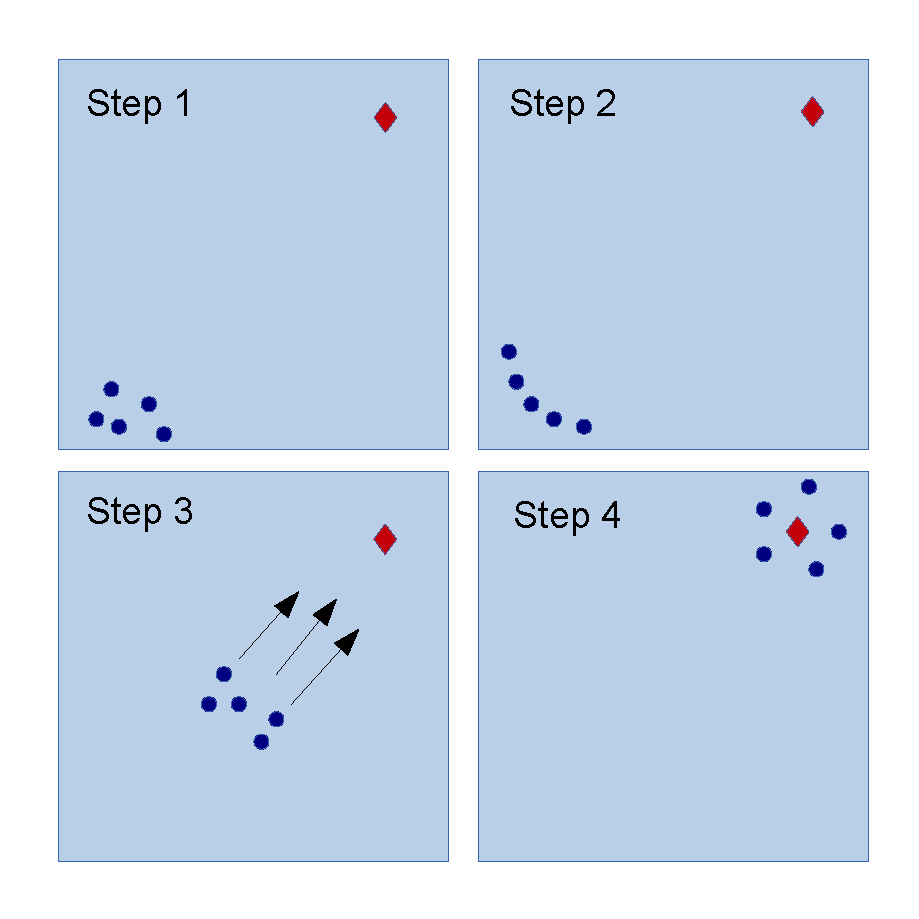
\includegraphics[width=75mm]{problemoverview.pdf}
\caption{Problem overview}
\label{problemoverview}
\end{figure}

The end goal of this work is a fully autonomous distributed system that is able to detect and locate \gls{RF} emitters without human intervention. In order to reach this goal, there are multiple stages with varying amount of information that has to be surpassed, in order to successfully locate the emitter. Breaking the system down to smaller pieces has the advantage of making each step possible to analyse separately, and as such, reducing the complexity of the task. Locating an unknown \gls{RF} emitter can be broken down in the steps seen in Figure (\ref{problemoverview}).


The different phases can be described as:
\begin{itemize}
\item Step 1 - Exploration of the search area and initial detection
\item Step 2 - Rough location-prediction
\item Step 3 - Effectively relocate sensors and converge on the emitter
\item Step 4 - Optimal location-prediction/closing in on the emitter
\end{itemize}

\newpage


In Step 1, none of the \glspl{UAV} have detected a signal using their sensors. In other words, the signal may be absent or out of range. Using methods from artificial swarm intelligence combined with a number of \glspl{UAV}, it is possible to search a large area quickly and efficiently. This is covered in the master thesis by Jørgen Nordmoen \cite{jorgenmaster}

Once at least one of the \glspl{UAV} in the swarm detect the emitter/comes within range of the emitter, it is able to call out for help, letting other members of the swarm come to aid in the search. At this point, it is assumed that the \glspl{UAV} are able to detect the signal, but do not have more than a vague indication of location of the emitter. For this work, it is assumed that there is only \textit{one} emitter. Due to the nature of signal propagation, it will be possible for the system to assume that the emitter is within a relatively restricted area. The size of the area is given by the frequency and the strength of the emitter. Under the assumption of an unknown \gls{RF} emitter, the emitted signal-strength will not be known to the swarm of \glspl{UAV}.  

Since the emitter can be restricted to a relatively confined area, we can apply another method of geolocating \gls{RF} emitters. This method is based on the \gls{RSS} of the signal. Using the differences in \gls{RSS} at different positions, it is possible for the swarm, as a unit, to estimate the location of the emitter. This is known as \gls{PDOA} algorithm. A minimum of three samples from different positions are required for this method to be applicable. The accuracy of the predictions, as given by the \gls{PDOA} algorithm, will vary based on the receiver configuration and noise in the environment. Noise can be filtered using filtering methods, but it is impossible to remove the noise completely. The positions of the receivers, in this case the \glspl{UAV}, can be optimized to minimize the error in prediction. 

Unfortunately, minimizing the error in prediction requires optimizing a non-linear and fairly complex system. This is hard, if not impossible, using analytic methods. An idea was conceived to use \gls{AI} methods, in particular a \glspl{GA}, to make it possible to find good strategies and configurations for receivers in finite time and using less computational resources. This is the basis for this project assignment and master thesis.

In the project assignment, Step 2 and Step 4 was explored. Step 2 is when a detection of an emitter has occurred and some indication of its location is required (Subsection \ref{P2RPC}). In Step 4, pinpoint accuracy of the emitter is required, and the receivers/\glspl{UAV} assume a configuration around the emitter to achieve this (Subsection \ref{P1FC}). 


\newpage
It would be wise to maximize the utility of the samples the \glspl{UAV} inevitably will collect during the transition from Step 2 to Step 4. This involves optimizing the flight path of multiple \glspl{UAV}, to maximize emitter prediction precision while minimizing resource consumption (flight time). To summarise, make an optimal decision about the flight path and actions of multiple \glspl{UAV} using limited information from Step 2, and minimize the resource consumption. Step 3 and associated problems are covered in this thesis.

The thesis also contains additional exploration of the problems discovered in the project assignment, specifically anomalies in predictions. This is documented in Section \ref{RA_FL} of this thesis. Noise and ambiguities significantly complicate many of the optimizations in this work. Initial experiments in the thesis work therefore explored why ambiguities occur, and what could be done to make solutions more robust, leading up to Step 3 and the optimization of paths.

A significant part of this work consists of well-chosen optimizations, chosen to provide insight into the important factors in precise geolocation of an unknown \gls{RF} emitter. Numerous scenarios and optimizations were created in this work. Those presented here are only some of the optimizations developed. In order to provide a concise and well-defined structure to this thesis, not all optimizations could be included. A master thesis is also time restricted. This leads to situations were optimizations have to be kept reasonably short in order to stay within the allotted time-frame, and allowing for more than one iteration with feedback from supervisors.




\newpage

\chapter{Background}

This chapter seeks to provide some background information for the different fields this report covers. This chapter is not a comprehensive knowledge-base for this study, but should give the reader the background needed to follow the rest of the report. 
\newpage
\section{\Glsentrylong{UAV}}

In general, there are many types of \glspl{UAV}, ranging from micro-sized surveillance helicopters, to large fixed-wing long-range autonomous planes. They all have one factor in common: the pilot, if any, does not have to be located in it or even near it. This allows for a lowering of cost, as human resources often are at a premium. 

For the purpose of geolocation of \gls{RF} emitters, \glspl{UAV} can be divided into two groups:

\begin{itemize}
\item Flying platforms that are able to hover
\item Flying platforms that are not able to hover
\end{itemize}

Whether a platform can stand still or not is important because a moving platform adds additional requirements to the rest of the hardware, in terms of real-time processing and fast refresh rates. A platform that can hover has the benefit of being able to follow an arbitrary flight pattern, but at the cost of endurance, in most cases.

\glspl{UAV} are able to provide functionality, previously only available to those willing and able to commit a large amount of resources. There is an ever increasing number of applications for \glspl{UAV}, both in civilian and military context, mainly due to reduced cost associated with the use of \glspl{UAV}. These are only some of the possible applications of \glspl{UAV}:

\begin{itemize}
\item Real-time monitoring of assets
\item Journalistic coverage
\item Disaster relief and recovering
\item Geolocation and rescue of missing persons
\item Relay-station for communications
\end{itemize}

As cost continues to decline, other applications for groups of \glspl{UAV} will become viable. Groups of \glspl{UAV} have the benefit of being able to decentralize and distribute a task across many units. Quite a few tasks can be very challenging to solve, given only one \gls{UAV}. However, a greater number of \glspl{UAV} would allow such tasks to be solved with greater ease. One such application is the geolocation of \gls{RF} emitters. This task is normally performed by a number of different techniques, as described in Section \ref{GTFUE}. 

\newpage

In short, there are two options for geolocating \gls{RF} emitters:

\begin{enumerate}
\item Specialized and expensive sensor equipment
\item Large number of general and cheap sensors
\end{enumerate}

One specialized sensor is not necessarily better than a group of general and cheap sensors. Combining this with the use of \glspl{UAV} leads to a highly mobile and versatile platform. In addition, the sensors will get better signal-to-noise ratio at higher altitudes, as will be described in Section \ref{RFPM}. \glspl{UAV} provide both mobility and the elevated platform, making it an excellent choice for a sensor platform.


\section{\Glsentrylong{RF} propagation modelling}
\label{RFPM}
\gls{RF} signal propagation is very complex. Some of the contributing factors to the \gls{RF} environment are:
\begin{enumerate}
\item Antenna properties: gain, directionality, size etc.
\item Free space loss: dampening of signal intensity, due to increasing area of coverage
\item Frequency of transmission: high-frequency signals are more easily dampened by environmental factors
\item Physical objects: trees, buildings etc. cause reflections and dampen signals
\item Weather, especially rain
\item Interference from other signals
\end{enumerate}

Estimating and properly including all of these factors into a propagation model will not be feasible in any reasonable amount of time. There are far too many contributing factors to be able to perfectly simulate the propagation of a signal through space. I, therefore, have to simplify and approximate these factors by an appropriate model. The model I used in this work is called the Log-distance \gls{PL} model \citep{saunders2007antennas}. This model gives the loss in signal strength, or received intensity at distance $d$ from the emitter. 


\begin{figure}[H]
\centering
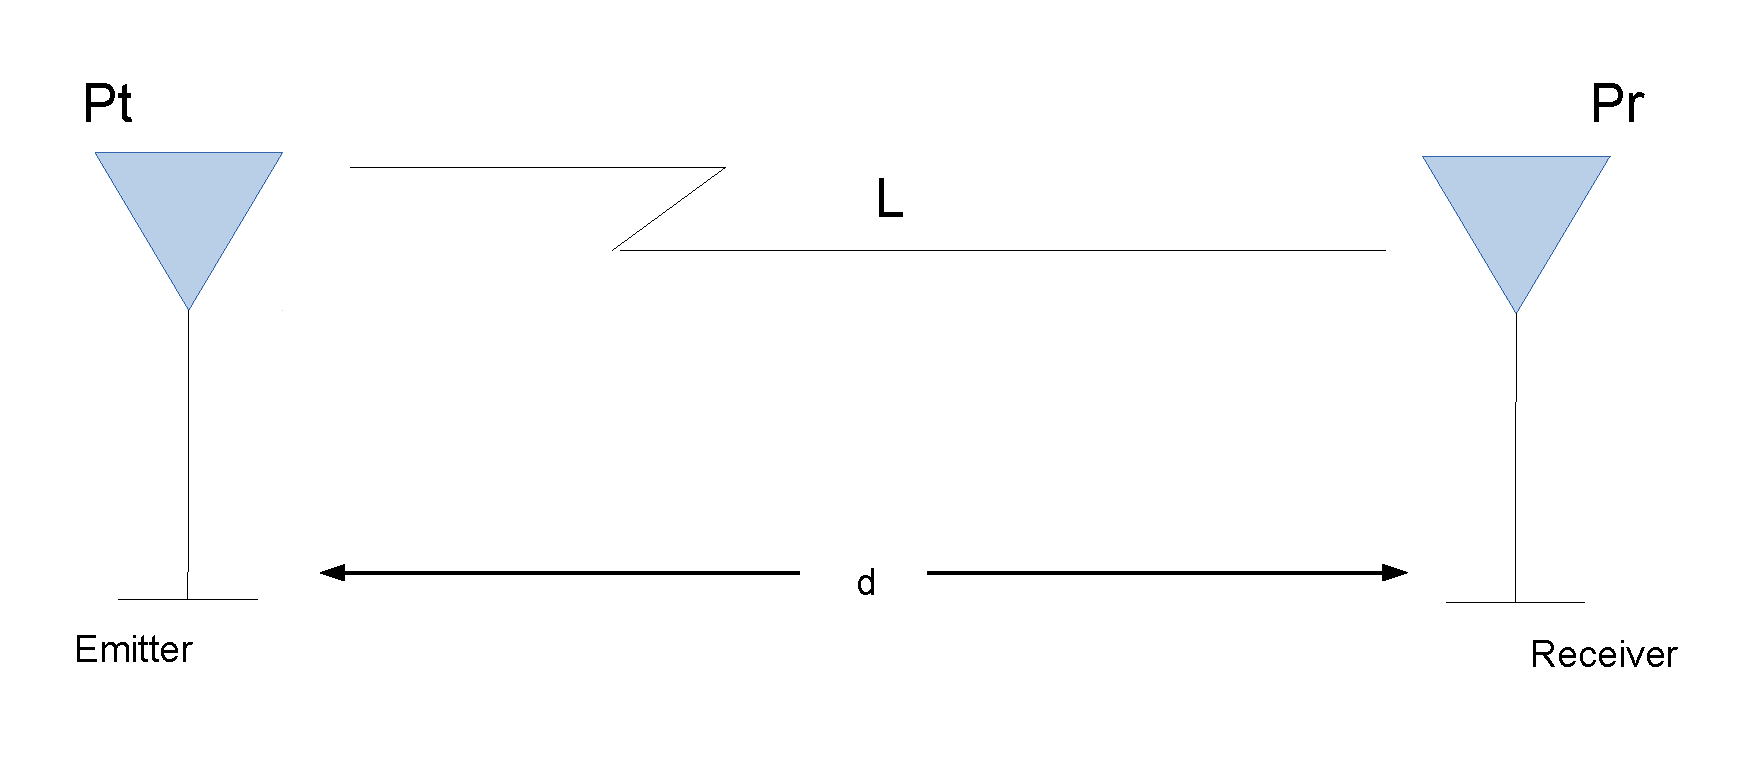
\includegraphics[width=90mm]{pathlossemitterreceiver.pdf}
\caption{Signal loss from emitter to receiver}
\label{pathlosstransmitterreceiver}
\end{figure}

$Pt$ is the emitted signal strength. $L$ is the loss in signal strength from emitter to receiver. $Pr$ is the received signal strength. $d$ is the distance from the emitter to the receiver. \Gls{PL} is the loss in signal intensity; from the figure this is given by the following equation:

\begin{eqnarray}
 P_r &=& P_t - L\\
 L &=& P_t - P_r
\end{eqnarray}


$L$ refers here to the loss due to the distance the signal travels from the emitter to the receiver. Commonly, this is approximated using this formula (unit is dB unless specified):

\begin{eqnarray}
 L(d) = L_f(d_0) + 10 \alpha \log \cfrac{d}{d_0}
\end{eqnarray}
$L_f(d_0)$ defines the loss at a given reference distance $d_0$. This is used because the signal propagation often does not conform to the model close to the emitter. Estimating $L_f(d_0)$ may be done empirically for real systems, however approximations exist. For the purpose of this work, the exact value of $L_f(d_0)$ is not important. It is a constant and is cancelled out where it is used (Section \ref{PDOANLLS}). 


$L(d)$, the loss in signal strength at a distance $d$ from the emitter, uses a parameter $\alpha$. $\alpha$ is the \gls{PL} exponent for the given environment. A higher $\alpha$ results in a greater attenuation of signal power. In free space, where the only cause of signal strength loss is the signal dispersion itself, $\alpha$ is equal to 2.0. In a real environment, where other factors are likely to contribute, $\alpha$ may vary from 2 to 6.

\begin{figure}[H]
\centering
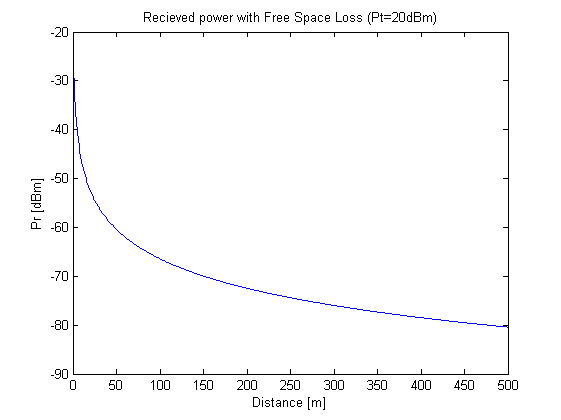
\includegraphics[width=85mm]{Pathloss.png}
\caption{Log-distance \acrfull{PL} model}
\label{pathlossnonoisegraph}
\end{figure}

Figure \ref{pathlossnonoisegraph} is a plot of the received signal power ($Pr$) against the distance from the emitter. The signal power drops rapidly at first, and then tapers off. This directly effects the detection range, as receivers are often specified at a certain sensitivity. Sensitivity refers to to the minimal detectable signal power the sensor can distinguish from noise.


\begin{figure}[H]
\centering
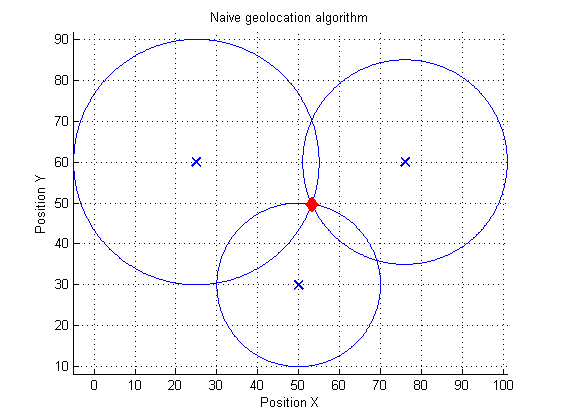
\includegraphics[width=85mm]{Intersectingcircles.png}
\caption{Naïve geolocation algorithm. Intersecting circles}
\label{naivegeolocationalgorithm}
\end{figure}

A naïve geolocation algorithm could use the $P_r$ directly by correlating the recorded signal strength with the distance. This could be done by inverting $P_r$ so that, given an \gls{RSS}, a distance from the receiver is returned. Each reading of the \gls{RSS} would then give a distance to the emitter from the sensor's position. Combining multiple sensor-readings would result in a set of circles which intersect at the emitter-location. 



The naïve approach to geolocation assumes that we know the strength of the signal sent by the emitter. This is often not a viable assumption, as emitters may not wish to be found. Emitters that do not wish to be found can use this assumption to mask their actual position by varying their signal-strength. An emitter that does not behave predictably does not give information to help locate it or is little known about, is said to be an uncooperative emitter. As a result, a robust geolocation algorithm cannot make any assumptions concerning the emitter's signal strength and has to consider the emitter uncooperative. 

The assumption made about $\alpha$ and the propagation model can be tested empirically. As part of a summer internship at \gls{FFI}, I worked with a group conducting a set of experiments to show that the assumptions reflect the real world \cite{ffireport2014}. The figure below depicts real measurements following the Log-Distance \gls{PL} model. As can be seen from the figure, depending on the height of the observation, $\alpha$ may vary. The green samples were taken at a height of 10m above ground level, resulting in a lower $\alpha$ than the blue samples. The blue samples were measured at ground level, which adds additional noise and reflections (which is modelled as a higher $\alpha$).

\begin{figure}[H]
\centering
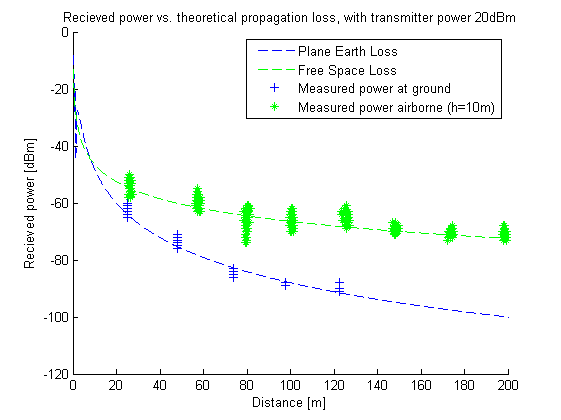
\includegraphics[width=80mm]{Pathlossrealdata.png}
\caption{Real-world data: signal strength vs distance }
\label{pathlossreal}
\end{figure}

The model, as presented here, is not exact - it leaves out many contributions that can affect the received signal positively or negatively. All the remaining contributions are appended as noise. This noise is modelled as a Gaussian stochastic variable $X$ with zero mean and variance that depends on the environment. Real-world trials have found the variance to be anywhere from 5dB to 15dB \cite{saunders2007antennas}. In most of this work, only a small amount of noise is used (1dB). It is assumed that a rolling average or some other filtering method is applied before attempting to predict the emitter-location.


\begin{eqnarray}
 L(d) = L_f(d_0) + 10 \alpha \log \cfrac{d}{d_0} + X\label{ldnoise}
\end{eqnarray}


\begin{figure}[H]
\centering
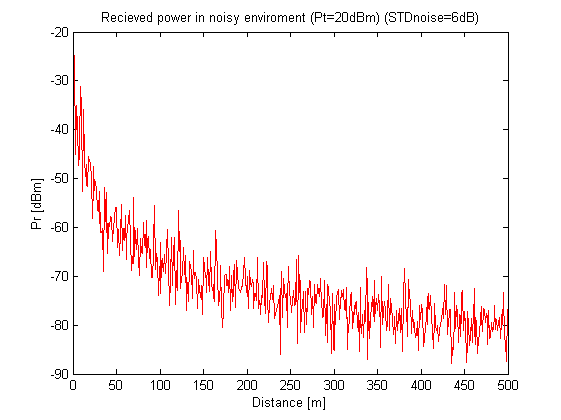
\includegraphics[width=90mm]{Pathlosswithnoise.png}
\caption{Log-distance \acrfull{PL} model with noise}
\label{pathlossnoisy}
\end{figure}

Figure \ref{pathlossnoisy} shows the Log-distance \gls{PL} with noise added (6dB). The addition of noise is of high importance. Noise with a high variance can cause an emitter to appear significantly closer or further away (it adds or subtracts to the signal power). Clearly, this is a major problem for any geolocation algorithm based on \gls{RSS}.  Adding noise makes it impossible to use the naïve approach of inverting Formula \ref{ldnoise} to get the distance to the emitter. Hence, other options for geolocation has to be considered.

\newpage
\section{Methods for geolocating objects }
\label{MFLO23S}

%todo A large amount?

A large amount of research has been conducted in the area of predicting positions of objects in 2D and 3D space \cite{srinivasan2007survey}. Some of the methods that can be used include:

\begin{enumerate}
\item Triangulation
\item Trilateration
\item Multilateration
\end{enumerate}

Triangulation refers to using direction to an object from a number of known points to estimate the position of the object. Using angles to get a position estimate has the benefit of giving a general direction, even with only one known point-reading. Adding another known point would give a position estimate in 2D space. A third point would be needed for 3D space. Alternatively, if we are only interested in a 2D position in 3D space (for example in the case where Z is 0 and the emitter is assumed to be on the ground), only two points would be required for a position estimate. The introduction of noise in the angular measurements would make the lines in Figure \ref{triangulation} cones instead, effectively giving an intersecting area, instead of a single point.

\begin{figure}[H]
\centering
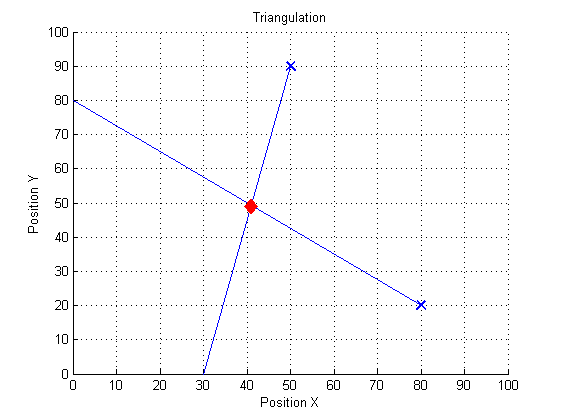
\includegraphics[width=90mm]{triangulation.png}
\caption{Triangulation in 2D space using two known points}
\label{triangulation}
\end{figure}

Trilateration will predict the position of an object by looking at distance to other known points. This is equivalent to drawing circles with radiuses equal to the distance to the object and examining where they intersect. If noise was introduced in the distance measurements, the circle-radiuses as seen in Figure \ref{trilateration}, would become thicker. As for triangulation, it would give an intersection area instead of a single point.

\begin{figure}[H]
\centering
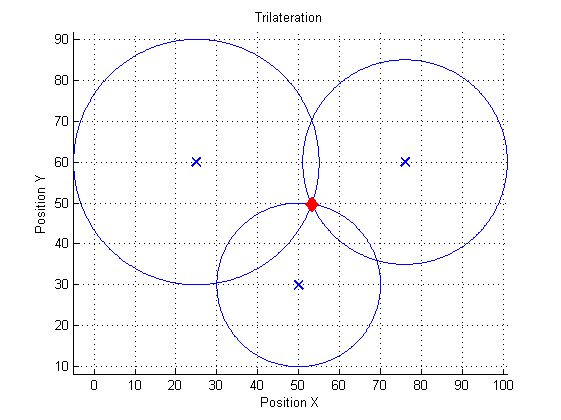
\includegraphics[width=90mm]{trilateration.png}
\caption{Trilateration in 2D space using three known points}
\label{trilateration}
\end{figure}

\citet{berle1986mixed} suggests using both triangulation and trilateration, as this would be beneficial in cases where either method is inaccurate on its own, or the object being located is attempting to deceive the geolocation algorithm. In this work, I apply previously defined algorithms directly. Using a combination of methods for geolocation is left as a topic for future exploration, and outside the scope of the current work.

\newpage
Multilateration looks at the difference in distance to the object measured from two or more known points in space. This will give a number of possible locations, which can be narrowed down by using more reference points. 

\begin{eqnarray}
D_{12} &=& | D_1 - D_2 |\\
D_{13} &=& | D_1 - D_3 |\\
D_{23} &=& | D_2 - D_3 |
\end{eqnarray}

$D_1$, $D_2$ and $D_3$ are the distances to the unknown point from the respective reference points $1$, $2$ and $3$, which are not known. If they were known trilateration could be applied. All that is known are the differences $D_{12}$, $D_{13}$ and $D_{23}$. 

\begin{figure}[H]
\centering
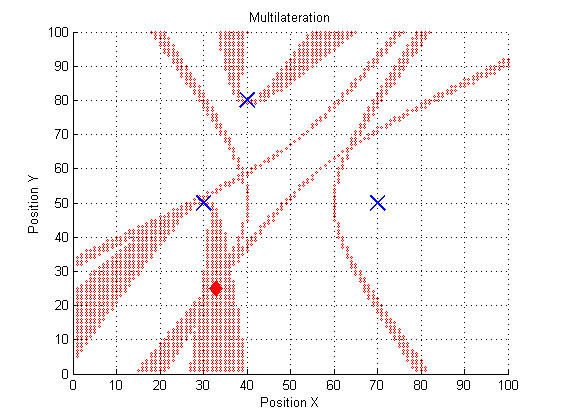
\includegraphics[width=90mm]{multilateration.png}
\caption{Multilateration in 2D space using three reference points}
\label{multilateration}
\end{figure}

The points in red are possible locations of the emitter, given that we know a set of distance-differences $D_{12}$, $D_{13}$ and $D_{23}$. By combing a set of these differences, it is possible to locate an unknown object by finding the points in space that satisfy all of the requirements. For instance, being $D_{12}$ distance closer to or further away from reference point 1 than reference point 2. Similar restrictions apply for all other pairs of reference points. Noise in the distance-differences would make the bands in Figure \ref{multilateration} wider, effectively, giving a larger intersection area where the object being located may be.

\newpage
\section{Geolocation of uncooperative emitters}
\label{GTFUE}

Locating an uncooperative \gls{RF} emitter is significantly harder than locating an emitter that cooperates. In a scenario where the emitter wishes to be found, the emitter could simply broadcast \gls{GPS} coordinates, making it trivial to find it. An uncooperative emitter may resist attempts to locate its position. This can be done by a number of techniques masking the true location of the emitter, such as varying signal strength, frequency hopping and burst transfers. A robust method for locating emitters should assume that the emitter is unwilling to cooperate in the search.

There are several techniques to locate an uncooperative \gls{RF} emitter. Among them are:

\begin{enumerate}
\item \acrfull{AOA} 
\item \acrfull{TOA}/\acrfull{TDOA}
\item \acrfull{FDOA}
\item \acrfull{RSS}/\acrfull{PDOA}
\end{enumerate}

\Gls{AOA} uses a highly directional antenna in order to get a directional vector for the emitter. Combining a number (at least two) of these sensors can give an estimate of position in two dimensions. 

\Gls{TOA} exploits the property of signal propagation, more concisely, it looks at the time when a signal was detected at one location and compares that to the time it reached another. This will, effectively, give an indication of where the signal is coming from.

\Gls{FDOA} makes use of Doppler-shift in order to give a reading of the emitter's position. Doppler-shift affects the frequency of the signal when moving towards and away from the emitter. A moving sensor may be able to use this to say something about the location of the emitter.

\Gls{PDOA} looks at the intensity of the signal. Given a suitable propagation model and a set of sensors, it is possible to estimate the position of the emitter, looking at only the difference in intensity of the signal received at multiple locations. \Gls{PDOA} has the advantage of being very simple to implement, requires little in terms of hardware, and the hardware required is widely available. For these reasons, I will be using the \Gls{PDOA} method for this study.

Multiple algorithms for \gls{PDOA} exist. The project assignment explored: \gls{NLLS}, \gls{DPD} and \gls{ID}. \Gls{NLLS} was chosen for giving the best predictions \cite*{jackson2011emitter}.

\newpage

\section{\glsentryshort{PDOA} algorithm: \glsentrylong{NLLS}}
\label{PDOANLLS}
\gls{NLLS} is a non-linear estimator of emitter-location. It is based on comparing measured difference in \gls{RSS} between two sensors, to a calculated/expected estimate of the difference given an emitter-location, and squaring the result. This can be used to give an emitter-location prediction, since the true emitter-location will result in a lower error than any other position. The non-linear property of the underlying mathematical equations makes the problem hard to solve analytically. \Gls{NLLS} is therefore used with a grid that specifies the possible prediction values for the algorithm. 

A two-dimensional grid is commonly used, however, there are no restrictions that would prohibit an extension to three dimensions. The prediction precision is directly tied to the granularity of the grid itself. A more finely grained grid will also lead to longer computation time for the algorithm to give a prediction. This means that trade-off between prediction precision and computation time is required. Exploring the trade-off between grid granularity and computation time is outside the scope of this work.

\begin{eqnarray}
P_{kl} &=& P_k - P_l \label{Pkl}\\
Q(x,y) &=& \sum_{k<l} [P_{kl} - 5 \alpha \log (\cfrac{(x-x_l)^2 + (y-y_l)^2}{(x-x_k)^2 + (y-y_k)^2})]^2\label{NLLSQxy}
\end{eqnarray}

Consider a set of sensors S. For each pair of sensors in S, the difference in \gls{RSS} ($P_{kl}$) can be calculated. $P_{kl}$ is the actual difference in measured signal strength. It is possible to derive an expression for the expected difference in \gls{RSS} for a pair of sensors, given the location of the emitter. This can be seen as the second part of formula \ref{NLLSQxy} ($5 \alpha \log (...)$). Squaring the deviation between the two differences, we have a measure of how well the sensor readings conform to the \gls{PL} model, given the emitter-location (x,y). 

\begin{equation}
\min\limits_{0\leq x\leq m}( \min\limits_{0\leq y\leq n} Q(x,y))\label{NLLSMin}
\end{equation}

$Q(x,y)$ can be considered a measure of how well the emitter-position (x,y) fits with the given sensor readings. By minimizing $Q(x,y)$ over a suitable grid, the most likely emitter-position (x,y) can be determined.


\newpage

\section{\Glsentrylong{GA}}

Taking inspiration from nature has led to many breakthroughs in artificial intelligence (ref swarm intelligence \citep{bonabeau1999swarm,kennedy2001swarm}, particle swarms \citep{eberhart1995new,shi1998modified}, neural networks and \glspl{GA} \citep{eiben2003introduction,goldberg1988genetic}). \Glspl{GA} is a way to simulate evolution within a computer. Evolution is a very powerful way of finding good solutions (not necessarily great solutions) to very hard problems that may even border what we can attempt to fully understand. Unlike solving a problem analytically, using a \gls{GA} only requires a measure of testing and comparing which solutions are better than others. Like evolution in nature, genes are passed from parents to children. The better fit an individual is, the greater the chance of that individual having its genes passed down. Mutation is added on top of this to optimize already good solutions and introduces a random element. Together, this makes up the \gls{GA} in its most basic form.

A \gls{GA} can be said to be a directed search: more exploration is performed in areas that show promise and have high fitness. This search is conducted by a population of possible solutions; each of these solutions is usually a complete, valid solution to the search problem. The \gls{GA} will optimize the solution on the basis of their fitness. The fitness of a solution is a single value (often a real number or integer). The absolute value of the fitness of an individual in the population is of little interest. How the fitness value compares (higher or lower) to the rest of the individuals in the population, will determine the given individuals' success. Indirectly, this specifies which genes are passed on and are considered viable for future exploration of the search space.

A simple \gls{GA} can be expressed in the following steps:

\begin{enumerate}
\item Create a random population of individuals
\item Calculate the fitness of the individuals in the population
\item Select some individuals from the population for mating; these are considered the parents 
\item Create a new set of individuals based on the ones previously selected (the children)
\item Mutate the children based on some (low) probability
\item Calculate the fitness of the new individuals and combine the children with the parent generation
\item If the desired performance of the population as a whole has been reached, stop executing, else go back to step 3

\end{enumerate} 


The \gls{GA} has been used on a number of real-world problems. As described above, it lacks any domain-specific knowledge needed to solve the given problem. Tailoring it to a specific problem involves defining the following properties:

\begin{enumerate}
\item Genome and phenome (a common decomposition of an individual)
\item Fitness-function
\item Crossover and mutation-operators
\end{enumerate}

Beginning with the genome, this can be compared to DNA in nature, which encodes the properties and acts as a recipe or blueprint. A common and simple genome representation is a bit-string. A number of bits may be combined to form a gene, which defines one property or value of the phenome. The phenome is the matured individual, and can be said to be the expression of its genes. The relation between genome and phenome acts as an abstraction layer, allowing the specification of a solution space that is easier to work with and may not include many or any invalid solutions. By careful design of the phenome-genome relation it is possible to restrict the \gls{GA} to solutions that are within the boundaries set by the problem. 

Consider a problem where the goal is to find the best usage of a single room, given a set of activities with durations (scheduling). Best usage would be a schedule that allows for as many as possible of the activities to be run without colliding. Having a way of mapping from one search space that does not have to consider the case of overlapping activities (invalid solution), would greatly simplify the problem. By encoding the schedule as start-time for each activity, it would be possible to schedule two activities so that they overlap. If one instead used an encoding based on the ordering of activities, this would not be possible. Problems that are more complicated often feature similar restrictions that could cause invalid solutions. The point is: a good genome-phenome relation may significantly reduce the size of the solution space by removing invalid solutions.

As mentioned previously, the fitness-function is the measure of how fit an individual/phenome is. This measure should be defined in such as a way that it accurately describes the problem at hand. Modelling complicated real-world problems to give a good relation between the fitness-values and the performance of the solution can be challenging. Far from all problems can be modelled in a simple way to allow for easy verification of the solution to the problem, but an accurate fitness-function is vital to enabling the \gls{GA} to solve the problem. For problems that do not have an easy way of estimating the performance of an individual/phenome, simulation may be the only option. 

Using simulation in the fitness estimation adds further challenges due to the (often) stochastic nature of the simulation. This problem may be illustrated by selecting the dice that gives you the best roll from a crate of dices. Each dice can have a different start value and number of sides, making the values produced by a random roll in the long run different for each dice. Picking a single dice and testing it may result in a very high value for a single roll, however, it is not given that this is repeatable, nor representable for the long-time performance of that dice. Solving this problem could be done by rolling each dice a number of times to make it more statistically significant, however, this takes more time. Each generated genome (which is then "evolved" into a phenome) has to be evaluated at least once. Having a fitness-function that is time-consuming to evaluate will clearly slow down the exploration of the search space, and thereby the problem-solving itself.

The two operators, mutation and crossover, create new genomes (children) from old genomes (parents). In general, there are some common choices for a crossover-operator, the simplest ranging from single-point crossover of the bit string, to complex methods of combining two tree-structured genomes. The single-point crossover selects a single index into the bit string. The bit strings from the parents are then split at that index, making two parts for each parent. Combining one part from each parent makes one child. 


How crossover is implemented is highly dependent on the internal representation chosen for the genome, but there are a few guidelines:

\begin{itemize}
\item Should include some part of each parent's genome, in most cases (a chance of just bringing the parents "as is" is sometimes used)
\item Often, a random element is included, for instance, the index in single-point crossover may be chosen at random
\end{itemize}

Crossover can, in early generations, do large jumps in search space by combining two solutions and retaining properties from both. Mutation is often a relatively small step in comparison. Mutation becomes an important factor in later generations, where crossover has little effect, as most individuals of the population are fairly similar. At that point, mutation can improve already good solutions, making them great, or help to get the solution out of a local maximum. Simplest form of mutation would be to flip some bits in the bit string of the genome, given a low random probability. More complicated forms of mutation are also possible, and can be tailored to better fit the solution space. For instance, searching for a solution in N-dimensional space could apply a small step in either of the N directions.

Choices for genome and phenome encoding are described in Subsections \ref{GP} and \ref{EAGENOMEPATH}. Information related to crossover  is found in Subsection \ref{EACROSSOVER}, and mutation in Subection \ref{EAMUTATION}.


\section{\Glsentrylong{MOEA}}


A \gls{MOEA}, is an evolutionary optimization-method, sharing most features of a regular \gls{GA}. Much like the \gls{GA}, the \gls{MOEA} has a concept of the genetic operations: crossover and mutation. There is little-to-no difference in the way crossover and mutation operates in a \gls{GA}, compared to that of the \gls{MOEA}. Crossover implementations, such as single-point or two-point crossover is applicable to a \gls{MOEA}

Fitness-evaluation for the \gls{MOEA} has one major difference compared to that of a regular \gls{GA}. A \gls{MOEA} optimizes on multiple objectives concurrently, and as such, each solution/phenome must be evaluated on multiple criteria. The output from a fitness-evaluation of a phenome is a list of values, representing the performance in the different criteria that are being optimized. 

For a \gls{GA}, the result of a run is a population of solutions with a single best-solution. When multiple objectives are being optimized at the same time, it is not possible to return a single best-solution. Instead, the \gls{MOEA} will return a set of solutions, known as a pareto front. The pareto front is a set of solutions, in which no solution dominates another solution in all criteria/objectives. Another feature of a solution on the pareto front, is that it is not possible to improve it in any objective without simultaneously decreasing the performance in another objective. It is important to understand, that the pareto front should span the entire spectrum of trade-offs between the objectives given. In effect, the pareto front highlights the best solutions, without giving preference to any of the objectives.

A \gls{MOEA} algorithm must try to maintain diversity in the solutions of the population to properly span the pareto front. This is done using an appropriate selection method. A commonly used selection method for \gls{MOEA} is the NSGAII \cite{deb2002fast}. Another method for selecting diverse individuals along the pareto front for mating is MOEA/D  \cite{zhang2007moea}. These differ in the way individuals are selected, and which individuals are selected to become the next generation.

As the \gls{MOEA} returns a set of solutions on the pareto front, additional choices have to be made if one wishes to be left with only one solution. Choosing the optimal trade-off between the objectives requires expert knowledge about the problem, or at least some preference on the trade-off between the objectives. It is not unreasonable to consider the \gls{MOEA}, an expert support system, aiding the decision maker in making good decisions. By highlighting and showcasing good solutions to the problem, many solutions that should not receive any attention from the decision-maker have already been excluded.






\newpage

\section{\Glsentrylong{FMM}}


The world is not normally distributed. Often, normal distributions can be applied with good results, but not always. Depending on the complexity of the distribution and how closely it resembles a normal distribution, it may be a reasonable simplification. Some distributions are too loosely related to the normal distribution to allow a normal distribution to make a good approximation. A fairly common example would be any type of multimodal probability distribution. Multiple peaks make a single normal distribution a rough approximation. 

By approximating real-world data to known distributions, it is possible to get a parametric model for the data. This can be extremely useful when attempting to interpret data. For multimodal distributions, it is not hard to imagine using multiple common distributions, such as a normal distribution, to model more complex shapes. This is what \gls{FMM} \cite{mclachlan2004finite} does: by approximating and fitting multiple distributions or components to the data, more complex data can be accurately modelled and parametric distributions created.

\gls{FMM} is not a new concept, but the recent advances in computer technology has increased the number of applicable use-cases. Given a set of data, the \gls{FMM} method is able to generate a parametric model. Only simple normal distributions are used as components for the \gls{FMM} in this work. \gls{FMM} requires some computational resources, as the components are fitted to the data using iterative steps. \gls{FMM} cannot guarantee an optimal fitting, but multiple random restarts can be applied to get better results. 

The number of components is given as an input to the fitting algorithm. This means that the user has to know how many components are required to model the data. Selecting the number of components is not always trivial. The result of too many components are wasted resources and an overly fitted model. Humans are skilled at detecting patterns and seeing tendencies, machines in general are not. Automating the selection of component-count can therefore be a challenge.

In this work, \gls{FMM} was used for visualizations in the Interactive simulator (Subsection \ref{M_INTER_FMM}). \Gls{FMM} was also used for clustering predictions in the Whack-A-Mole strategy (Subsection \ref{RA_HEUR_HEUR})





\newpage

\section{Related work}
\glsresetall

\subsection{General}

This section provides an overview over work done by others, that relates to the problems at hand. Not all of the presented work may, at first glance, seem to be of high relevance, however, it is the intention to provide the reader with references to other research that is applicable to this field of study.

\subsection{Comparison of \acrshort{PDOA} methods}

\citet{jackson2011emitter} at Defense Research and Development Canada has conducted an in-depth study and comparison of the different algorithms for \gls{PDOA}. Their work shows promising results, predicting the location of an emitter over a fairly large area. Additionally, they compared the computational intensities of the algorithms and their prediction precision. 

All their work was done on the ground, using a mobile measurement station, averaging samples over time. Being on the ground, they were subject to more noise than what would be the case if the measurements had been taken from an elevated platform.

\subsection{Geolocation of \acrshort{RF} emitters by \acrshortpl{UAV}}
 
\citet{scerri2007geolocation} from Carnegie Mellon University, did research and some practical work on \glspl{UAV} \cite{scerri2007geolocation,scerri2008transitioning}. They used a group of flying, fixed-wing planes in order to scan an area for \gls{RF} emitters, and implemented a method of effective path-planning for each of the \glspl{UAV}. 

\gls{BBGF} was used to give an estimate of the likelihood that any given location contains an emitter. New information from the sensors of the \gls{UAV} was used to update the \gls{BBGF}. The resulting output (from the \gls{BBGF}) was then used to make a map of entropy in the area. 

This map gives a view off which sample-readings would provide the most information and value to the model. Path-planning can then be conducted by maximizing the information gain or reduction of entropy in the model. Their structure allowed them to select the flight-path that gave the most information about the area.


\subsection{Optimal Landmark Selection for Triangulation}

\citet{madsen1998optimal} from the Aalborg University, compared different triplet-configurations, and gave an overview of the uncertainty in positioning, based on the triplet selected. Their work was based on a camera-based sensor and a set of known landmarks. The goal was for a robot to be able to use this information to give a good estimate of its own position at any given time.

\subsection{NASA antenna}

Antenna design is a challenging problem that has not yet been fully solved. Part of the problem is that antennas may perform very well without engineers being able to explain why. \citet{hornby2006automated} investigated this using an Evolutionary Algorithm to evolve an antenna for use on a space probe. They found that they could make antennas that were smaller and performed better than the currently known antennas. The only problem was that no one could explain why the antenna performed so well. Without fully understanding why it worked so well, it is considered high risk to use it for critical applications. NASA therefore could not use the antenna on their space probe. 

In their work, they used a relative recursive tree-like genetic encoding. This was adapted for use in this work and was used to encode the path of \glspl{UAV}. See Subsection \ref{EAGENOMEPATH} for details on the encoding used in this work. 



\chapter{Summary of the project assignment}

The thesis is the extension of a project assignment. This chapter is a summary of the work conducted as part of the project assignment. Introduction, background and methods for this work is covered in the respective chapters of the main report.
\newpage



\section{Introduction}

\subsection{Problem background}

The two problems I have looked at are related, however, also significantly different. In order to be able to find an emitter, a search has to be conducted. This search is not necessarily starting in a location where it is possible to get a direct reading of the emitter. It is also not given that we will be able to easily and without cost, move to check out every signal detected in the search. Therefore, a trade-off between precision of estimates and computational cost has to be made. First step towards a solution to this problem is to look at the following two problems:

\begin{enumerate}
\item The optimal configuration (freely placed) to gain best precision possible. Sensors will be able to assume a configuration around the emitter's actual location.
\item A configuration (sta ic) that gives best precision on estimates (using N = 3,4,6,.. receivers), given that the sensors have to remain in relative proximity to each other, and not have the emitter within the formation itself.
\end{enumerate}

Problem 1 is of interest, since it will effectively give an estimate of the precision, it is possible to achieve, given a \gls{PDOA} algorithm and a number of sensors. Furthermore, it may be of interest to see whether the trivial solution (a triangle, square or in general a ring) is, in fact, the optimal solution, given a freely placed configuration around the emitter.

Problem 2 represents a scenario where the emitter may just have been detected by one or more sensors. This means that the sensors will have no way to proceed, and an estimate with a reasonable precision from the current position will be of great value for future path-planning.

In order to make the problems above manageable, the following assumptions have been made:
\begin{enumerate}
\item A given configuration of N sensors can be said to be better (or worse) than another configuration of N sensors. Better or worse is given by a criterion such as estimate precision.
\item A sensor configuration may behave in a directional manner, meaning that it may exhibit properties making it non-uniform in its precision of estimate, depending on the location of the emitter.
\item The \glspl{UAV} are not allowed to use multiple samplings or averaging to remove noise from their readings. Noise is therefore a bigger problem than it may be in a real-world application
\item \glspl{UAV} are able to get an exact position-fix on its own location (with no noise).
\end{enumerate}

The sections that follow aim to provide a better granularity to the problems, by dividing them into questions that may be tested, or in other ways verified by the results in this report. 





\subsection{Problem 1: Free configuration}
\label{P1FC}
The main focus of this problem is to explore how accuracy is affected by the configuration chosen. Factors that increase or decrease precision of estimate are of particular interest. In order to be able to classify the solutions provided by the \gls{GA}, I will be using the trivial solution as a point of reference. The trivial solution, in this case, refers to putting all the available sensors in a circle around the emitter. For three sensors this shape would be a triangle.

Extending this, working with a higher number of sensors, seeing how well the solutions generalize and which factors are driving for the accuracy is important. In general, this can be described as: what is the value of adding another sensor to the set of receivers? Knowing this will allow for better decision-making in higher level planning, using groups of autonomous sensors.

Research questions:
\begin{enumerate}
\item Will the trivial solution (circle around the emitter) always be optimal in terms of error in position estimate?
\item How will the propagation environment affect the distance from emitter to sensor, given an optimal configuration?
\item Does the solution from (1) generalize to N sensors?
\item What is the value of adding another sensor?
\end{enumerate}


\newpage

\subsection{Problem 2: Remote pinpoint configuration}
\label{P2RPC}
Cost is often a driving factor in development and decision-making. In this problem, the cost of moving to an optimal position, such as in Problem 1 (Section \ref{P1FC}), is assumed to be high. Therefore, I wish to give a good location estimate with reasonable precision, without allowing the sensors to place themselves freely. 

The restrictions in place to achieve this are simple:
\begin{enumerate}
\item A circle is defined, within which the sensors may configure themselves freely.
\item This configuration is encoded in such as way that it is possible not only to relocate the sensors as a set (while maintaining their individual relation to each other), but also that the configuration may be rotated arbitrarily (Subsection \ref{GP}).
\end{enumerate}

Having these restrictions will allow for testing of the following research questions:

\begin{enumerate}
\item Does the configuration depend on the distance from the emitter?
\item Is the configuration found directional?
\item Is it possible to develop robust omni-directional configurations with good accuracy?
\end{enumerate}




\newpage

\section{Results}


\subsection{Problem 1}
\label{RP1}
\paragraph{Solutions}
\label{RP1SOS}
The solutions provided by the \gls{GA} are consistent for a low receiver count ($N = 3,4$). At 5 receivers, the solutions, as seen in the figure, is obtained in most cases,  as long as the \gls{GA} is left to run for long enough.

\begin{figure}[H]
\centering
\begin{minipage}{50mm}
\textbf{Cartesian coordinates:}
\end{minipage}%
\begin{minipage}{50mm}
\textbf{Polar coordinates:}
\end{minipage}
\begin{minipage}{50mm}
  \centering
  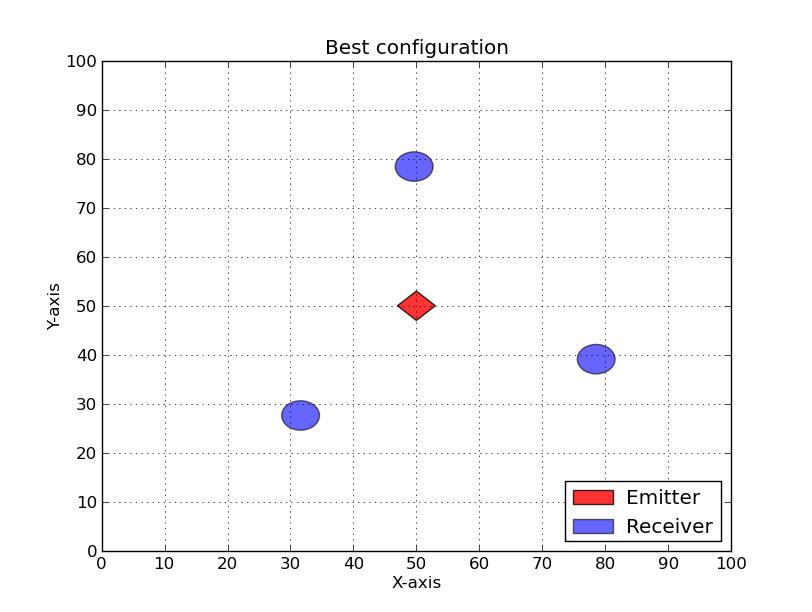
\includegraphics[width=50mm]{ConfigurationCart3Recv.jpg}
  Cartesian, 3 receivers
\end{minipage}%
\begin{minipage}{50mm}
  \centering
  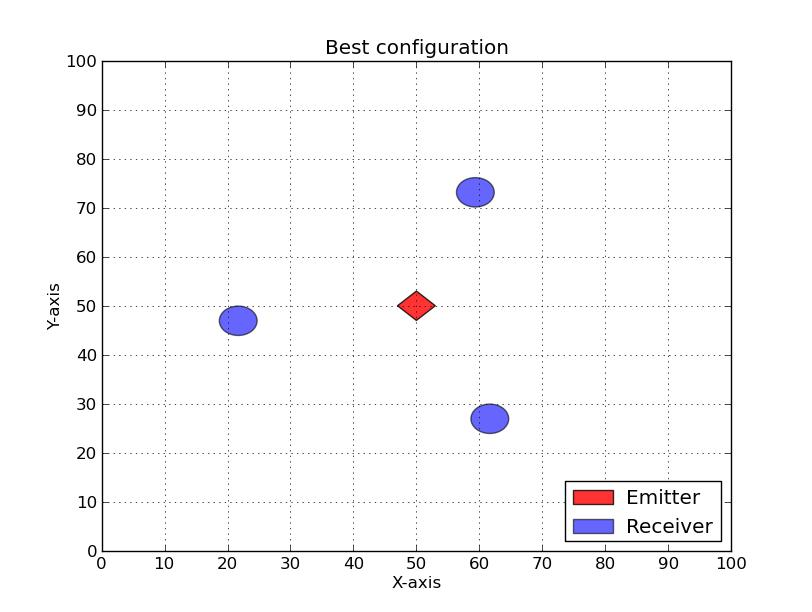
\includegraphics[width=50mm]{ConfigurationPolar3Recv.jpg}
  Polar, 3 receivers
\end{minipage}
\begin{minipage}{50mm}
  \centering
  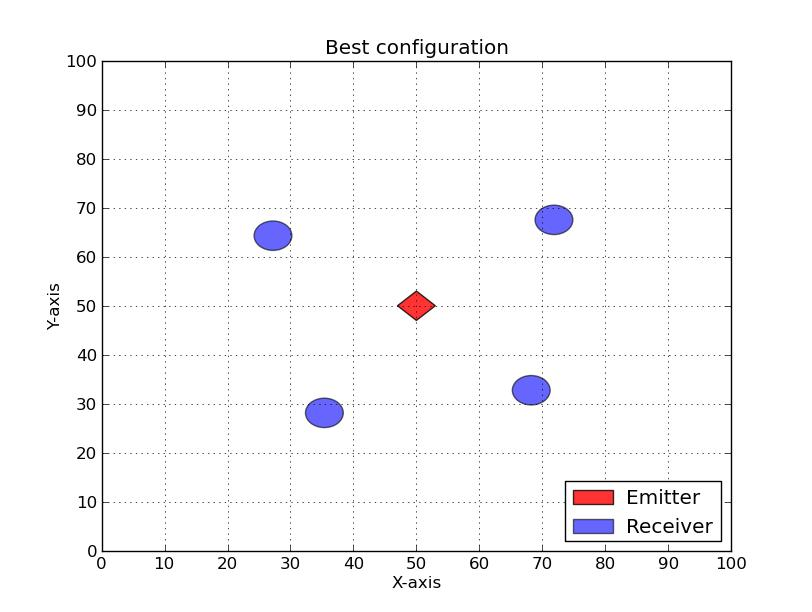
\includegraphics[width=50mm]{ConfigurationCart4Recv.jpg}
  Cartesian, 4 receivers
\end{minipage}
\begin{minipage}{50mm}
  \centering
  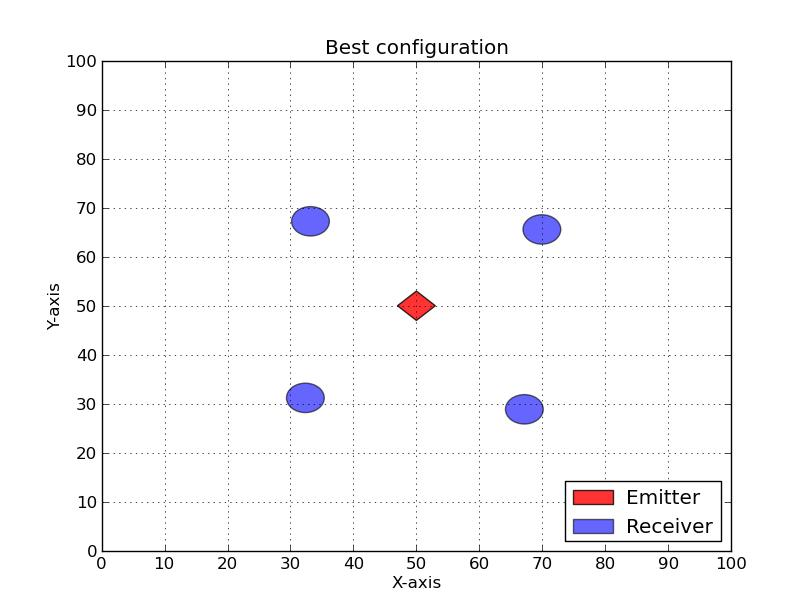
\includegraphics[width=50mm]{ConfigurationPolar4Recv.jpg}
  Polar, 4 receivers
\end{minipage}
\begin{minipage}{50mm}
  \centering
  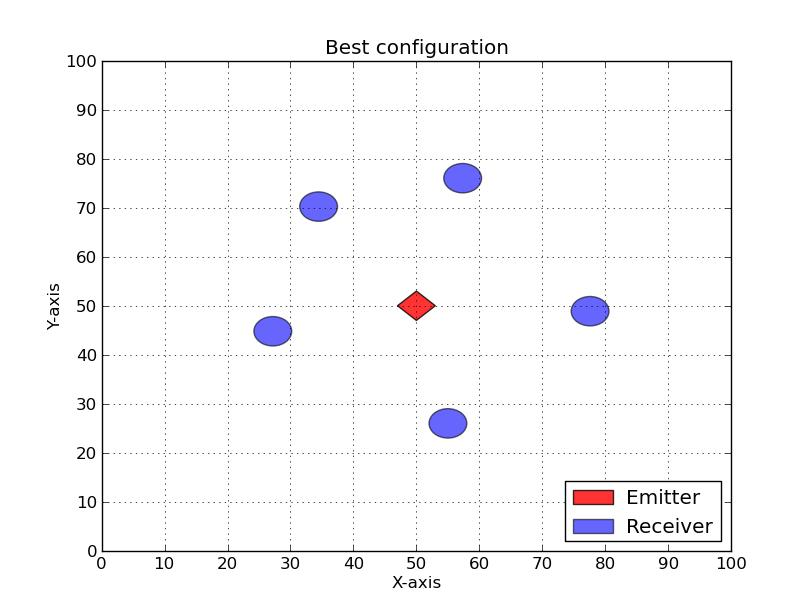
\includegraphics[width=50mm]{ConfigurationCart5Recv.jpg}
  Cartesian, 5 receivers
\end{minipage}
\begin{minipage}{50mm}
  \centering
  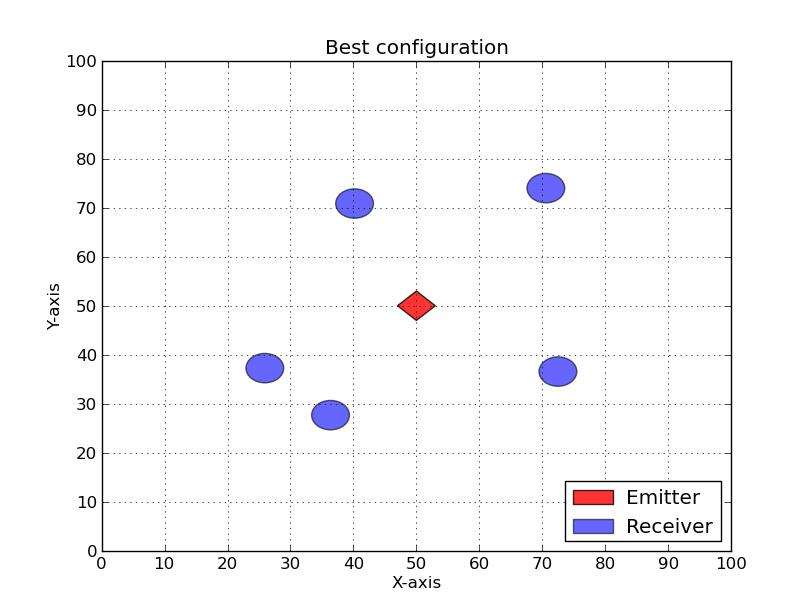
\includegraphics[width=50mm]{ConfigurationPolar5Recv.jpg}
  Polar, 5 receivers
\end{minipage}
\caption{Problem 1 - Comparison of formations (Cart. and Polar)}
\end{figure}


\paragraph{Prediction precision and receiver count}
\label{PPARC}
Problem 1 (Subsection \ref{P1FC}) describes a research question of finding the value of a receiver. In other words: the increase in prediction precision when adding another receiver. The value of a receiver can be defined by comparing the precision of the prediction with and without said receiver. Doing this for N = $3$,\ldots,$10$, it is possible to get an impression of what the receiver is worth. Note that including or excluding a receiver becomes a matter of comparing the optimized configuration for 3 receivers to the optimized configuration for 4 receivers. 

To give a fair comparison, all optimizations took into account that it is more computationally intensive to find a more complex solution. As such, finding the configuration for 10 was given significantly more computation time (generations and population size) than 8 or 9.

\begin{figure}[H]
\begin{minipage}{50mm}
\small
\begin{tabular}{c|l|l}
\textbf{Receivers} & \textbf{Error (m)} & \textbf{Gain (m)} \\ \hline
3 & 10.77 &  \\ 
4 & 7.04 & 3.72 \\
5 & 5.43 & 1.61 \\
6 & 4.47 & 0.97 \\
7 & 3.96 & 0.50 \\
8 & 3.82 & 0.14 \\
9 & 3.35 & 0.47 \\
10 & 2.56 & 0.79 \\

\end{tabular}
\end{minipage}
\begin{minipage}{80mm}
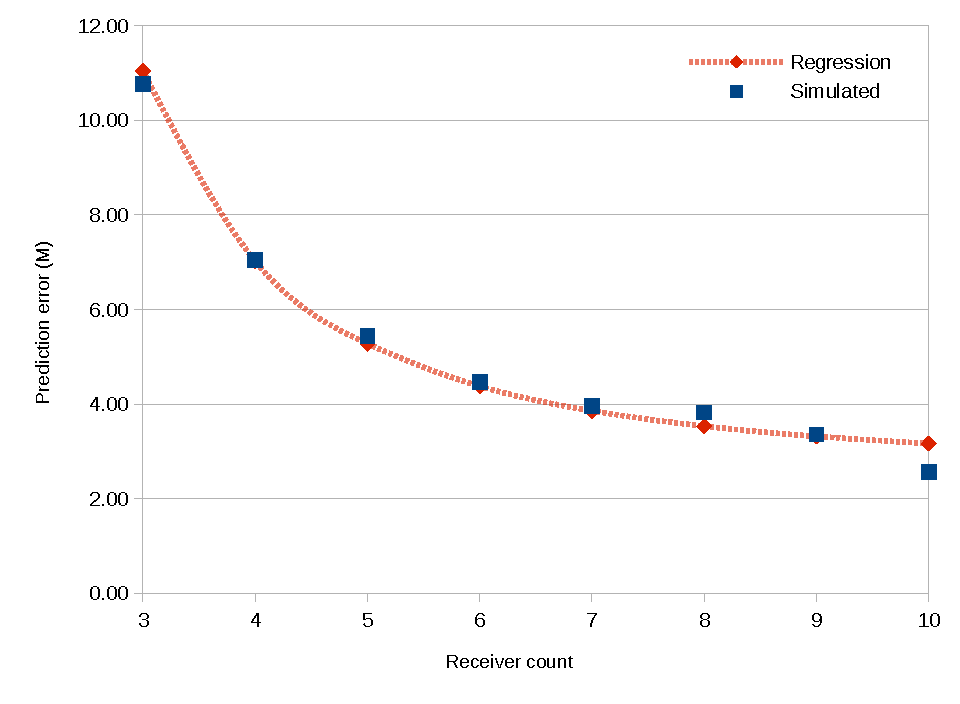
\includegraphics[width=70mm]{receivervalue.pdf}
\end{minipage}
\caption{Prediction error vs receiver count}
\label{predictionerrorreceivercount}
\end{figure}

As seen in the Figure \ref{predictionerrorreceivercount}, adding a receiver to a configuration of 3 receivers results in a significant decrease in location-prediction error. The gain of adding another receiver (going from 4 to 5) is much less than from 3 to 4. In other words, the absolute gain of adding another receiver is quickly with every added receiver.



\newpage
\subsection{Problem 2}
\paragraph{Explanation}

\label{RP2G}

As in problem 1, problem 2 attempts to evolve a formation of receivers to get accurate predictions of an \gls{RF} emitter. Unlike problem 1, problem 2 has restrictions on the possible/allowed placement of the receivers. Problem 2 has greater issues with stagnation and getting stuck in local optima. Even so, the \gls{GA} provides some insight into the better and worse choices that are possible to make when choosing a receiver-configuration, given the restrictions specified in Section \ref{P2RPC}. 

Problem 2 uses a slight variation of the fitness-evaluation from problem 1. There are two distinct types of formations being evolved:



\begin{enumerate}
\item Directional formations - formations that are allowed to develop an attachment to the relative direction of the emitter.
\item Robust omni-directional formations - formations that are rotated during fitness-evaluation to remove any attachment to the direction of the emitter (relative to the formation).
\end{enumerate}

It was quickly discovered that left unattended, and using the same measure of fitness as for problem 1, the configurations developed in problem 2 would become "weighted" towards the emitter. Rotation during fitness-evaluation was added to counter this effect. An example of this can be seen in Figure \ref{problem2norotaterecv6}.

\begin{figure}[H]
\centering
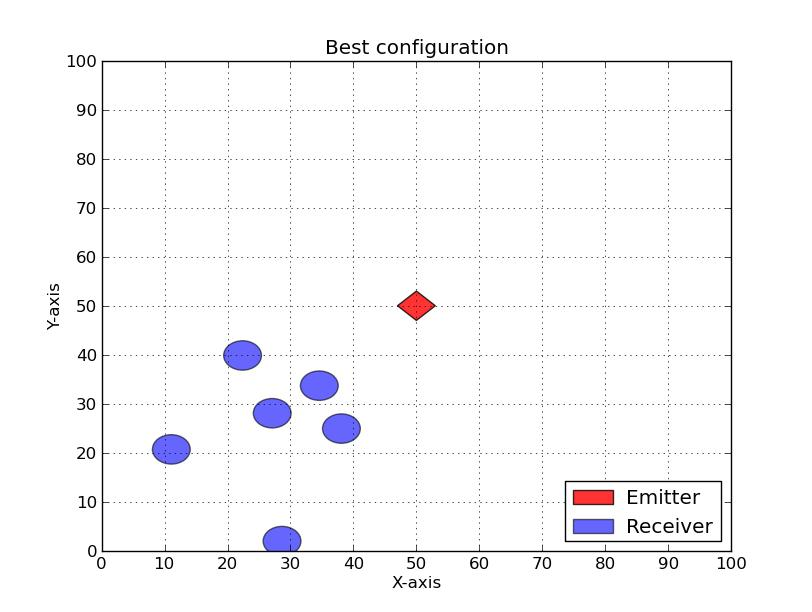
\includegraphics[width=90mm]{Problem2NoRotateRecv6_3.jpg}
\caption{Problem 2 - 6 Receivers, not rotated}
\label{problem2norotaterecv6}
\end{figure}




\paragraph{Solutions}
\label{RP2SOS}

Compared to problem 1 (Subsection \ref{RP1SOS}), the solutions generated for problem 2 show greater variation. This is likely due to the added difficulty of obtaining accurate position estimates when the receivers are not allowed to freely place themselves. In short, this results in less freedom and worse overall predictions than the free configuration from problem 1. This means that the fitness-values for all individuals in problem 2 are lower, and there is less span which could help the \gls{GA} to distinguish better solutions from worse. Multiple solutions were generated for each $N$ ($ = 3,\ldots,6$). They show some similarities, but it is difficult to draw general conclusions (Figure \ref{problem2comparison34receivers}).

\begin{figure}[H]
\centering
\begin{minipage}{50mm}
\textbf{3 Receivers:}
\end{minipage}%
\begin{minipage}{50mm}
\textbf{4 Receivers:}
\end{minipage}
\begin{minipage}{50mm}
  \centering
  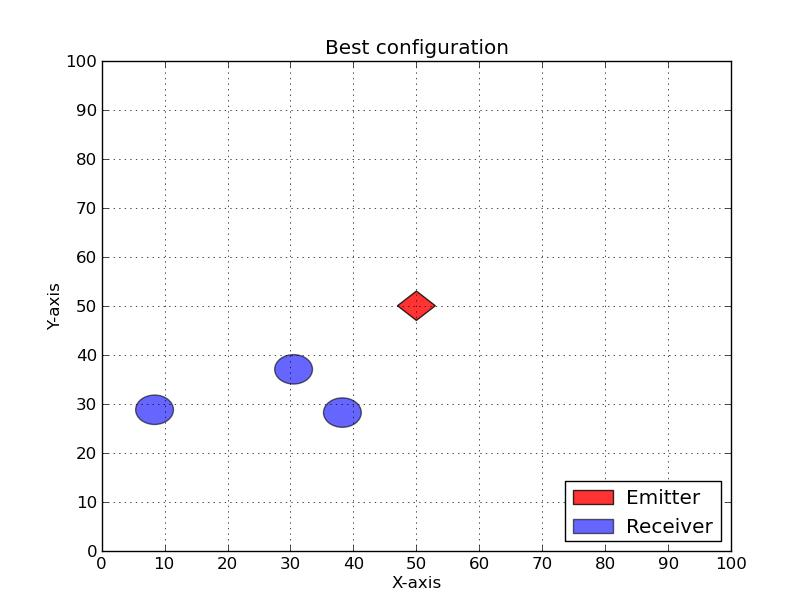
\includegraphics[width=50mm]{Problem2NoRotateRecv3_1.jpg}
  %Problem 2, 3 receivers
\end{minipage}%
\begin{minipage}{50mm}
  \centering
  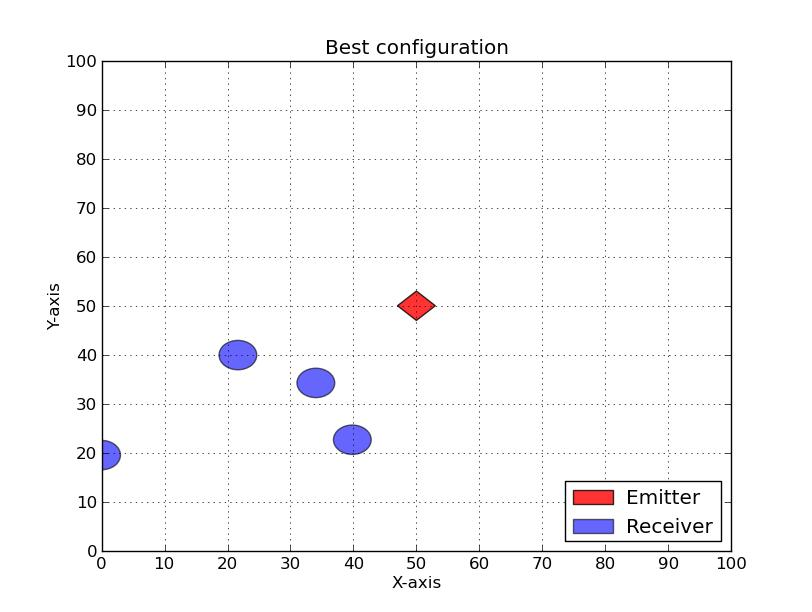
\includegraphics[width=50mm]{Problem2NoRotateRecv4_1.jpg}
  %Problem 2, 4 receivers
\end{minipage}
\begin{minipage}{50mm}
  \centering
  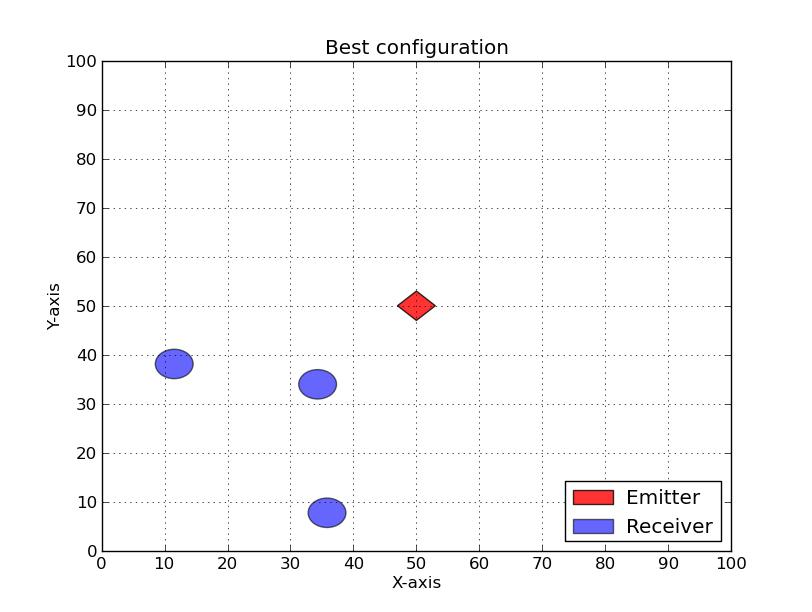
\includegraphics[width=50mm]{Problem2NoRotateRecv3_2.jpg}
 % Problem 2, 3 receivers
\end{minipage}
\begin{minipage}{50mm}
  \centering
  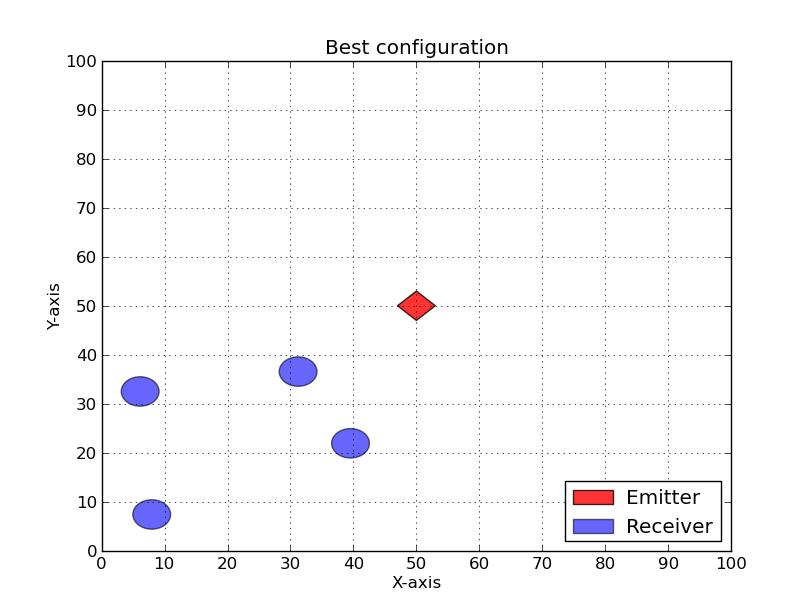
\includegraphics[width=50mm]{Problem2NoRotateRecv4_2.jpg}
  %Problem 2, 4 receivers
\end{minipage}
\begin{minipage}{50mm}
  \centering
  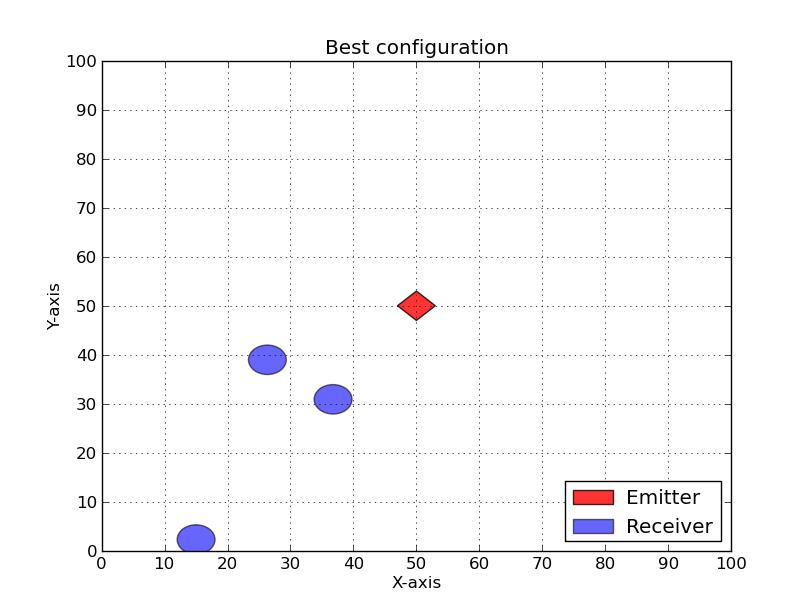
\includegraphics[width=50mm]{Problem2NoRotateRecv3_3.jpg}
 % Problem 2, 3 receivers
\end{minipage} 
\begin{minipage}{50mm}
  \centering
  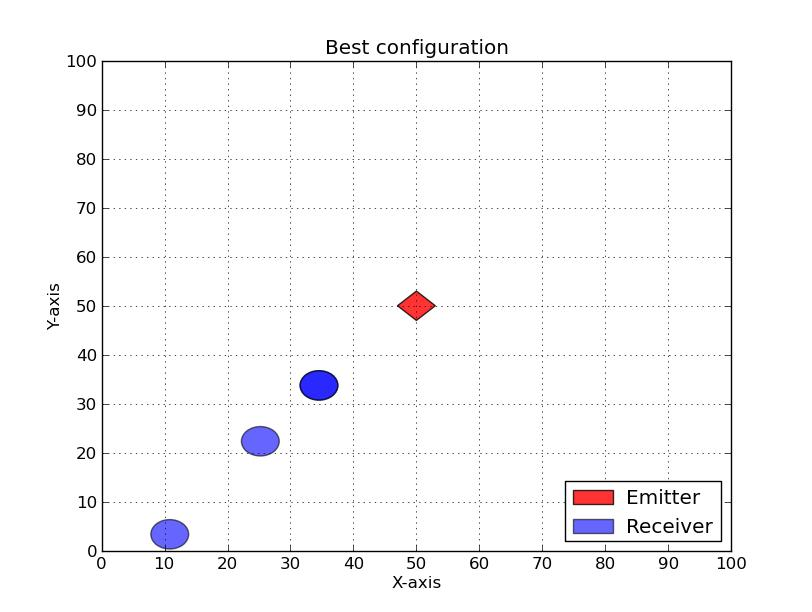
\includegraphics[width=50mm]{Problem2NoRotateRecv4_3.jpg}
  %Problem 2, 4 receivers
\end{minipage}
\caption{Problem 2 - Comparison of formations using 3 and 4 receivers}
\label{problem2comparison34receivers}
\end{figure}


\newpage
Starting from 5 receivers and up (Figure \ref{problem2comparison56receivers}), it becomes clearer that a set of receivers is always placed reasonably close the emitter. To offset this "weight" it was also common that the \gls{GA} placed some receivers further away. 


\begin{figure}[H]
\centering
\begin{minipage}{50mm}
\textbf{5 Receivers:}
\end{minipage}%
\begin{minipage}{50mm}
\textbf{6 Receivers:}
\end{minipage}
\begin{minipage}{50mm}
  \centering
  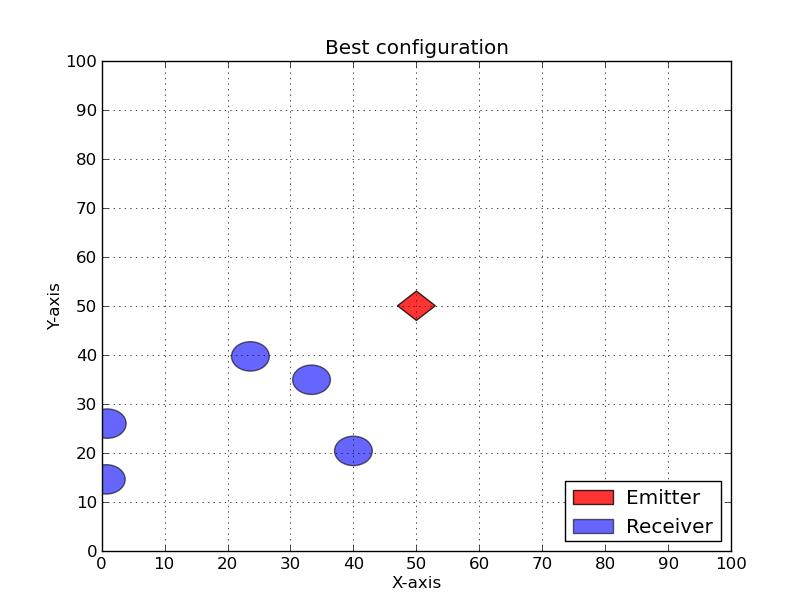
\includegraphics[width=50mm]{Problem2NoRotateRecv5_1.jpg}
 % Problem 2, 5 receivers
\end{minipage}%
\begin{minipage}{50mm}
  \centering
  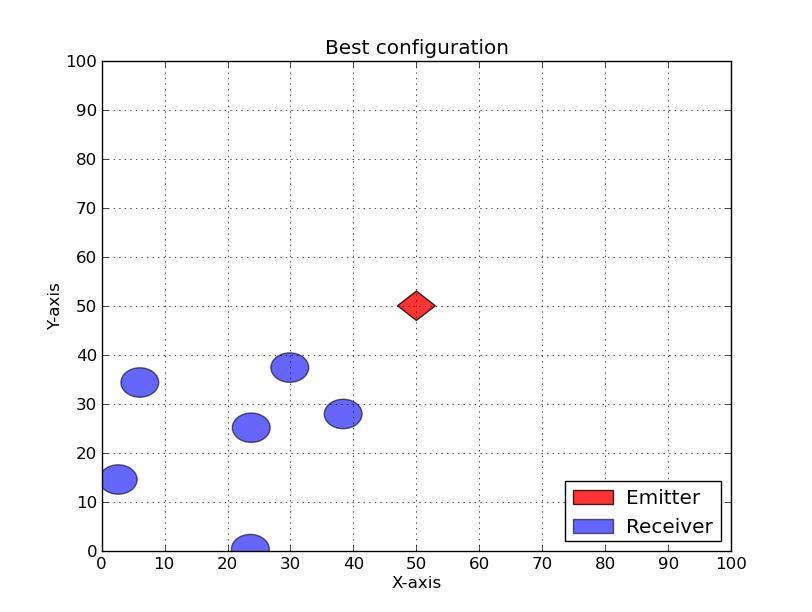
\includegraphics[width=50mm]{Problem2NoRotateRecv6_1.jpg}
  %Problem 2, 4 receivers
\end{minipage}
\begin{minipage}{50mm}
  \centering
  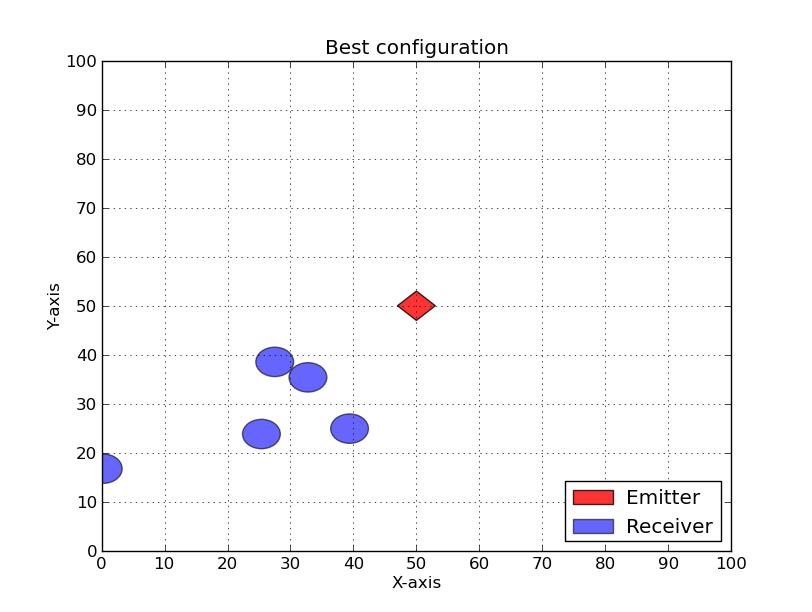
\includegraphics[width=50mm]{Problem2NoRotateRecv5_2.jpg}
  %Problem 2, 5 receivers
\end{minipage}
\begin{minipage}{50mm}
  \centering
  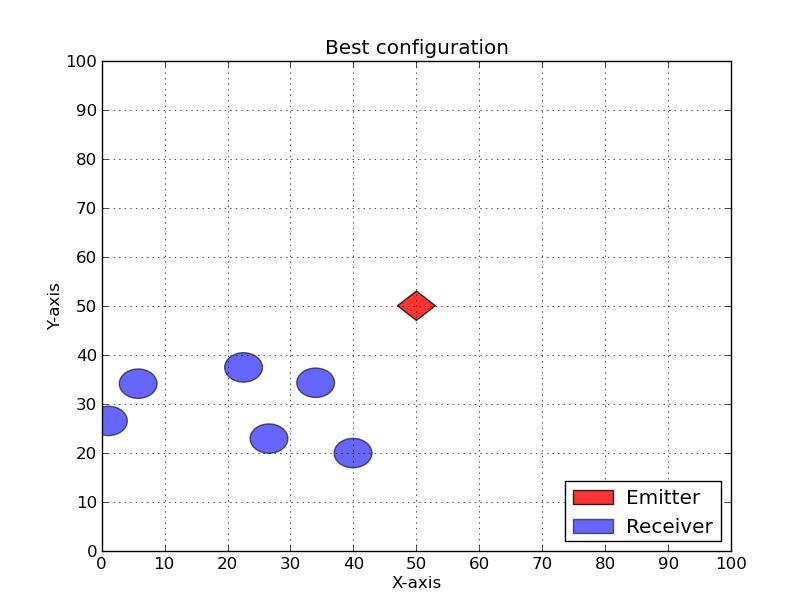
\includegraphics[width=50mm]{Problem2NoRotateRecv6_2.jpg}
  %Problem 2, 4 receivers
\end{minipage}
\begin{minipage}{50mm}
  \centering
  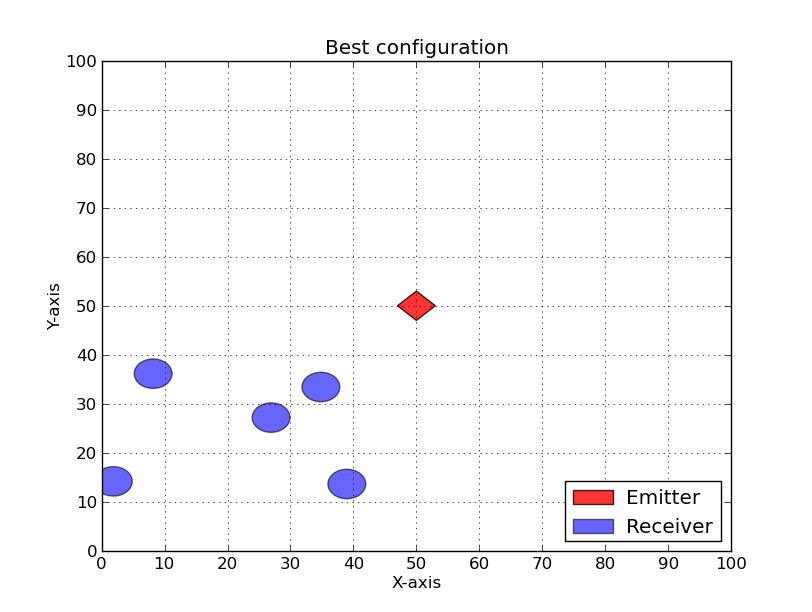
\includegraphics[width=50mm]{Problem2NoRotateRecv5_3.jpg}
  %Problem 2, 5 receivers
\end{minipage} 
\begin{minipage}{50mm}
  \centering
  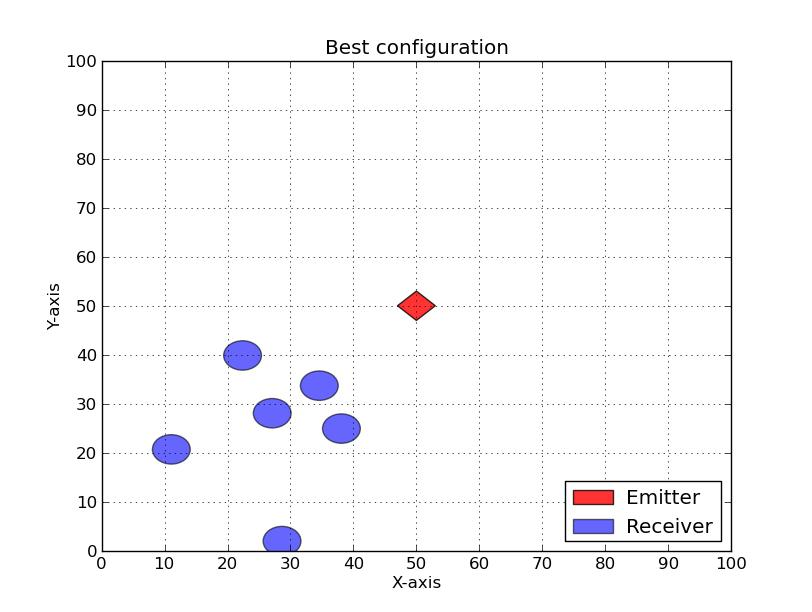
\includegraphics[width=50mm]{Problem2NoRotateRecv6_3.jpg}
  %Problem 2, 4 receivers
\end{minipage}
\caption{Problem 2 - Comparison of formations using 5 and 6 receivers}
\label{problem2comparison56receivers}
\end{figure}

\newpage

By introducing rotation of the formation as part of the fitness-evaluation, most of the asymmetries vanish. The formations are, by this operation, not able to evolve attachment to the direction of the emitter (relative to the formation). This can be seen in Figure \ref{problem2rotate}



\begin{figure}[H]
\begin{minipage}{60mm}

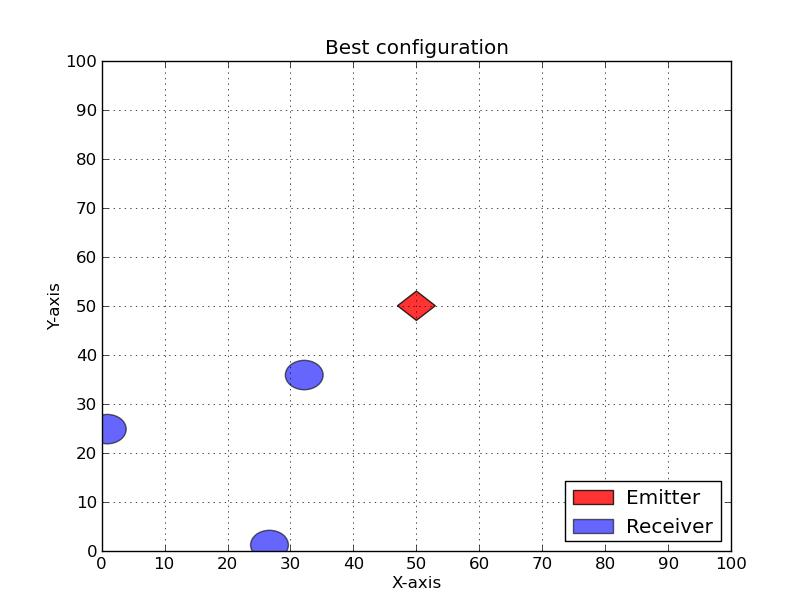
\includegraphics[width=60mm]{Problem2RotateRecv3.jpg}
\end{minipage}
\begin{minipage}{60mm}

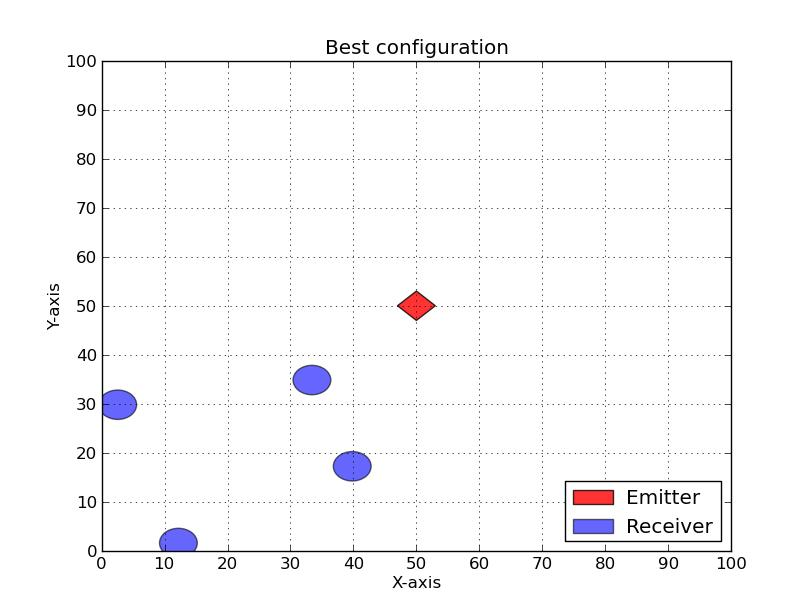
\includegraphics[width=60mm]{Problem2RotateRecv4.jpg}
\end{minipage}
\begin{minipage}{60mm}

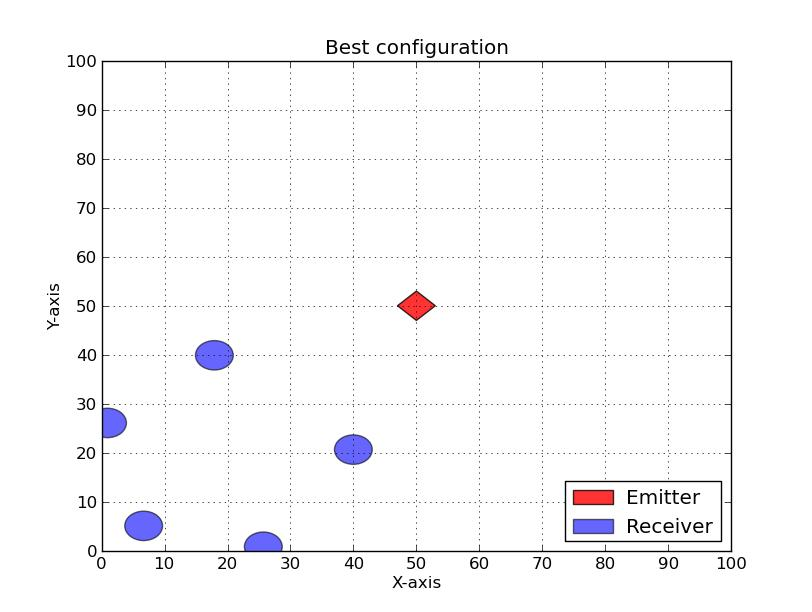
\includegraphics[width=60mm]{Problem2RotateRecv5.jpg}
\end{minipage}
\begin{minipage}{60mm}

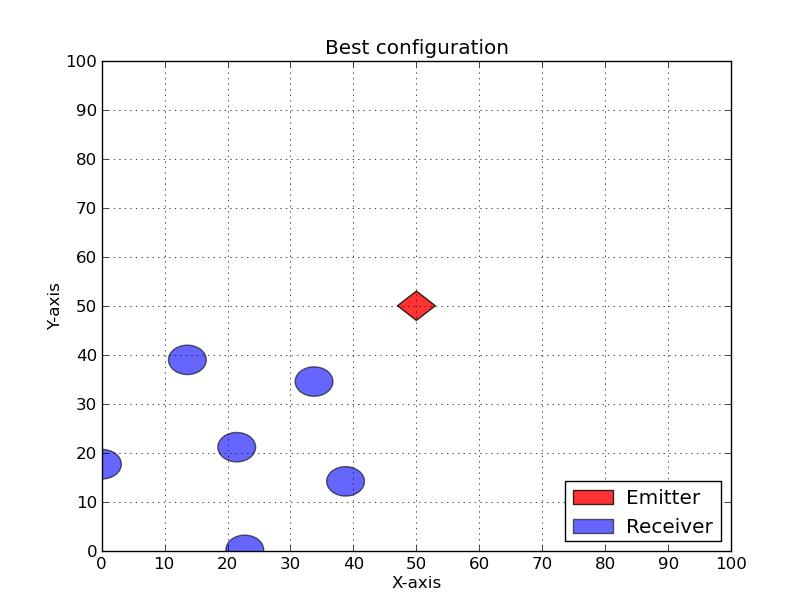
\includegraphics[width=60mm]{Problem2RotateRecv6.jpg}
\end{minipage}
\caption{Problem 2 with rotation}
\label{problem2rotate}
\end{figure}

For 3 and 4 receivers, the formations approach a triangle and a square, respectively. These formation makes the predictions independent of the direction of the emitter, relative to the formation. Configurations for 5 and 6 exhibit same symmetrical properties as for 3 and 4 receivers. 




\newpage

\section{Analysis}

\subsection{Problem 1}
\label{RP1GS}

Problem 1 consisted of finding the best configuration in terms of prediction precision and low error in estimates. In this problem, the receivers were allowed to place themselves freely around the emitter. A restriction on minimum distance to the emitter was set to avoid the receivers gathering on the emitter. Having the receivers gather on the emitter is not useful from a practical point of view. Not only would this alert the emitter to the fact that it has been found, but additionally, it could make the \glspl{UAV} crash into each other if they got close enough.

The initial assumption was that, given the ability to freely place themselves around the emitter, the receivers would form a circle. This was assumed to be the best option, as it would space the receivers out and therefore, provide the most "varied" samples while maintaining relative proximity to the emitter, which gives better signal strength. From the results (Subsection \ref{RP1SOS}), this appears to be the case, at least for 3, 4 and 5 receivers.

For receiver count $N$ = 3,4,5, each of the solutions appear to form a circle around the emitter. Some formations are more perfect than others, but this is accredited to fitness landscape being indifferent to slight asymmetries in the formation. As a note for future work, it may be possible to develop a better fitness-function to counter this and develop perfect formations. 

The problem with fitness indifference is further extended at higher numbers of receivers. Given a sufficient number of receivers, the predictions become very accurate, and the position of each individual receiver matters less. In practice, this makes optimizing receiver configuration with a high number of receivers difficult. One idea might be to scale the fitness-value in such a way that, once there is already a high precision and low error in prediction, a small change matters more (gives a more significant increase in fitness). At the moment, fitness behaves in a way that at first, given bad formations of receivers and high error in estimates, improvements are large. Changing the scaling of the fitness-values might help alleviate these issues.

In some cases, the \gls{GA} got stuck in local optima. This was countered by reseeding the \gls{GA} or by changing the parameters to be less elitist. Population size also plays an important role in maintaining population variance and avoiding stagnation. Performance-problems limited the size of the populations used. Better hardware or massive parallelization could help keep the \gls{GA} from stagnating. Often, in the solutions that stagnated, multiple receivers were placed on top of each other or close to each other; this behaviour could merit further investigation. 

The following research questions were presented as part of the problem specification in Subsection \ref{P1FC}:

\begin{enumerate}
\item Will the trivial solution (circle around the emitter) always be optimal in terms of error in position estimate?
\item How will the propagation environment affect the distance from emitter to sensor, given an optimal configuration?
\item Does the solution from (1) generalize to N sensors?
\item What is the value of adding another sensor?
\end{enumerate}

Answer, in turn, to each of the questions:

\begin{enumerate}
\item For a low number of receivers N = 3,4,5, the trivial solution of placing the receivers on a circle appears to be optimal. For a higher number of receivers, the trivial solution is also good, however, the \gls{GA} had issues distinguishing solutions due to indifference in fitness (many configurations has equal or similar fitness-value).

\item The propagation environment, noise and $\alpha$, each reduce the precision of location-estimate as they increase (as expected). Increasing the noise resulted in a lower baseline or best-fitness value possible to get, given a number of sensors. Increasing $\alpha$ makes the noise more visible and the location-estimates more sensitive to the noise (lower signal-to-noise ratio).

\item As problems were encountered when using many sensors/receivers (see 1), no certain conclusion can be made, in this case. However, nothing contradicts that the assumption of the solution from (1) could generalize to N receivers.

\item The value of adding another receiver depends on how many are already in place. Diminishing returns are present. More in-depth results on this question can be found in Subsection \ref{PPARC}
\end{enumerate}



\newpage
\subsection{Problem 2}

Problem 2 was about finding a formation of receivers that could estimate the location of an emitter remotely. As specified in Subsection \ref{P2RPC}, this configuration should not surround the emitter itself. This restricted the possible solutions. All solutions found for problem 2 are worse than an equivalent solution with the same number of receivers for problem 1. In other words, the additional restriction on receiver-placement comes at the cost of prediction precision. 

I will comment on the formations generated without rotation in the fitness-evaluation first, then move on to formations generated using rotation as part of fitness-evaluation. As stated in Subsection \ref{RP2G}, early convergence and stagnation was a problem for testing of problem 2. This lead to a variety of different configurations, with patterns (if any) being hard to detect. 

Realistically, similar logic as for problem 1 (Subsection \ref{RP1GS}) can be applied. Receivers benefit, in terms of prediction precision or reduced error in estimates, of spreading out. Having multiple receivers positioned close to each other may negate the value of the receivers, as they could have been replaced by a single measurement/receiver. 

My initial assumption was that the receivers would form a parabola towards the emitter in order to get the best accuracy of predictions. This appears to be partly true, as can be seen in the figures for 5 and 6 receivers (Subsection \ref{RP2SOS}).  In addition, some receivers appear to have been placed far from the emitter. This may be to counteract the weight of samples close to the receivers, and excludes the solution that the emitter is at the edge of the grid ($x,y = 0,0$). 

All formations generated seem acutely aware of the emitter being placed in the middle. Most, if not all of the configurations feature some centring or focus towards the center of the search area. This confirms the assumption that the direction in which the emitter is located affects the best configuration to locate it. In a real-world scenario, where the emitters-location is unknown and a group of \glspl{UAV} is trying to locate it, it is not viable to make assumption of the direction of the emitter. Unless, of course, this is done using alternate geolocation techniques, such as triangulation (Section \ref{MFLO23S}).

Now, I will take a look at the formations generated using rotation as part of the fitness-evaluation. These have become more-or-less completely symmetric, making them indifferent t the direction of the emitter. It appeared, early on, as if the formations generally would form a circle around a center-point, effectively arranging the receivers along the border of the area that was allowed. The formation of 6 receivers discredits this hypothesis by placing a receiver in the middle of the formation (radius $= 0$). It would have been interesting to investigate what would happen with more receivers ($N > 6$). Due to performance and time constraints this was not possible.

It was assumed that, restricted to a small area away from the emitter, the receivers would form some type of parabola to get the best prediction in the direction of the emitter. This was found to be the case, given that the formation was allowed to evolve an affinity towards one direction (not rotated during fitness-evaluation). Research questions for this problem can be found in Subsection \ref{P2RPC}, and are listed below:

\begin{enumerate}
\item Does the configuration depend on the distance from the emitter?
\item Is the configuration found directional?
\item Is it possible to develop robust omni-directional configurations with good accuracy?
\end{enumerate}

Some of the questions proved more challenging than others to answer. This was mostly caused by instability of the \gls{GA} in converging on a singular solution. Instead, the \gls{GA} produced a set of solution that varied significantly (Subsection \ref{RP2SOS}). In turn, the answer to the research questions:

\begin{enumerate}
\item Attempting to test this by moving the emitter revealed unforeseen dependencies to the grid-size and test setup. This made it impossible to test this sufficiently, as the \gls{GA} would get stuck in local minima. The reason for it getting stuck is assumed to be related to the fitness-measure, and is material for future studies.
\item The configurations found are highly directional. As can be seen in Subsection \ref{RP2SOS}, they exhibit a parabolic shape in the direction of the emitter. 
\item Developing a robust omni-directional configuration was done by including rotation of the receiver-formation in each fitness-evaluation. Examples of configurations generated can be found in Subsection \ref{RP2SOS}.
\end{enumerate}


\newpage


\chapter{Methods}

This chapter aims to provide insight into the methods used, and how the results were achieved. It will provide a general overview over the work that went into this study, and should make it possible to reproduce the work.

\newpage


\section{\Glsentrylong{CUDA}}

\subsection{Hardware}


\begin{figure}[htp]
\centering
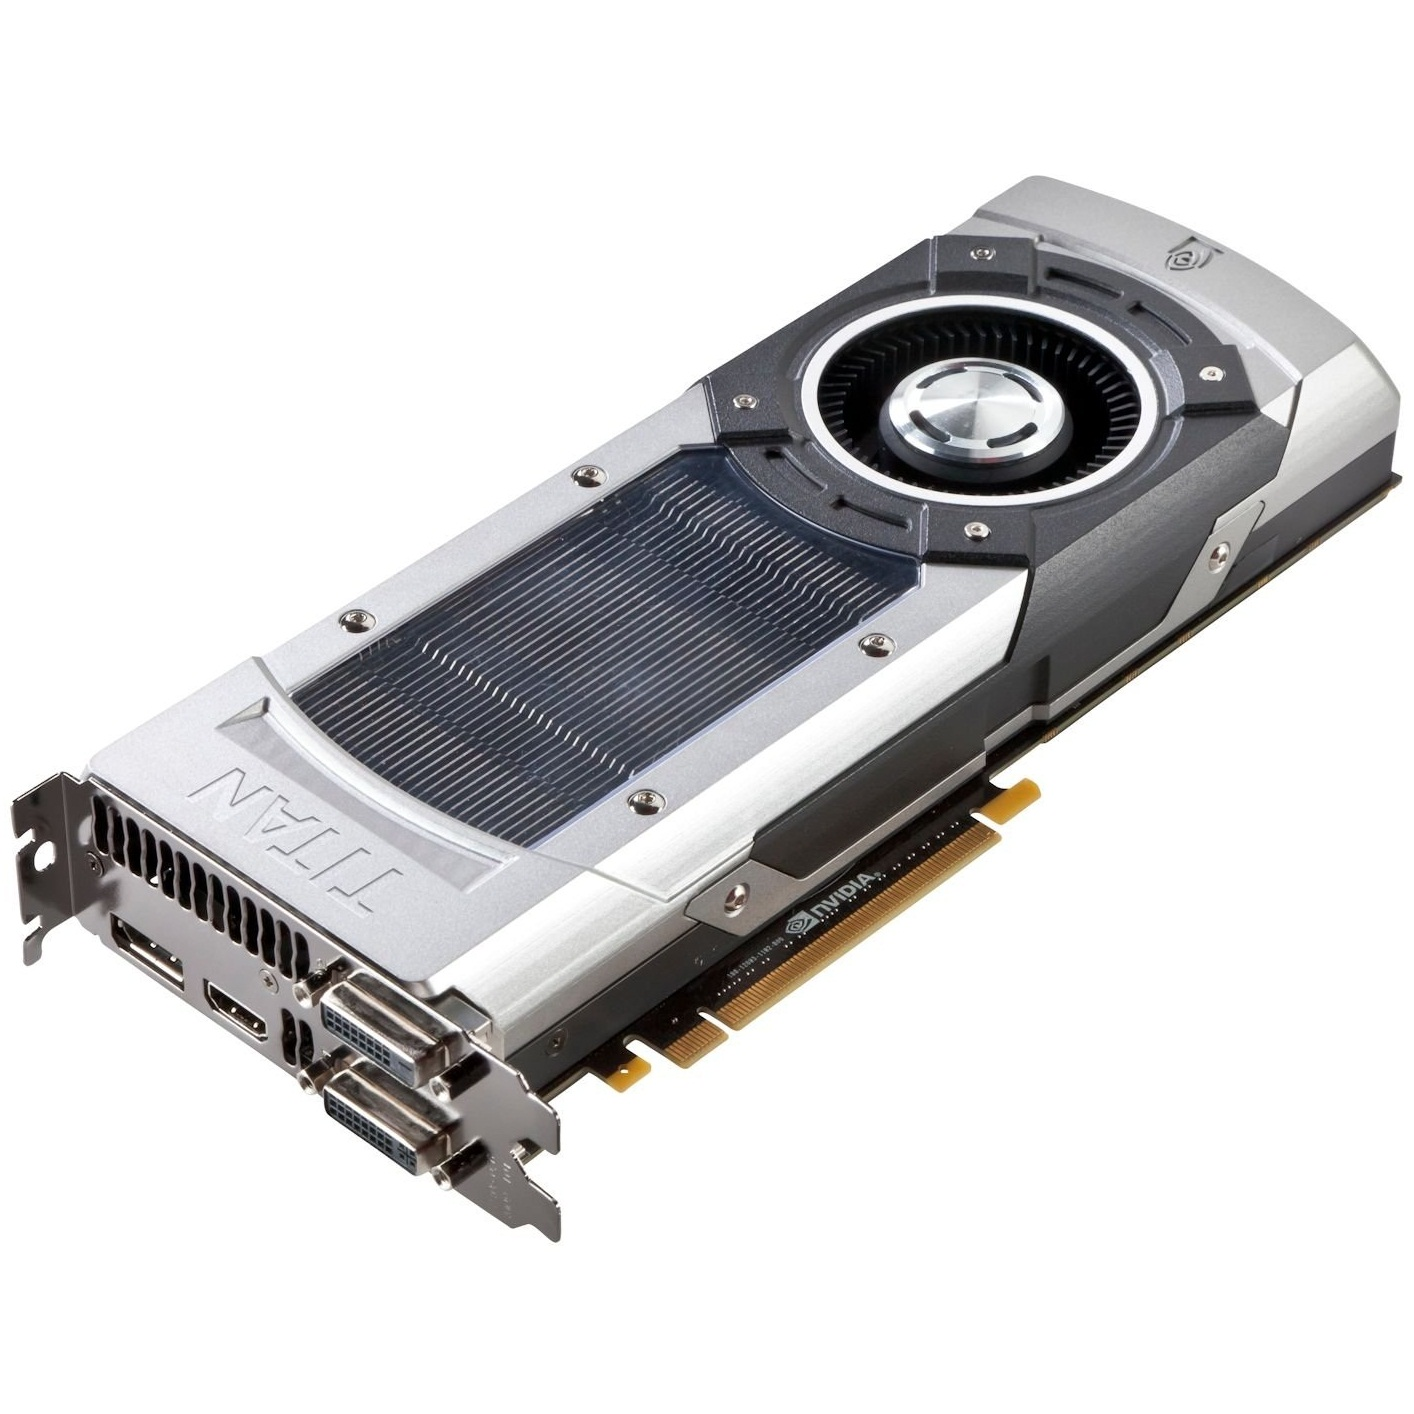
\includegraphics[width=60mm]{geforcetitan.jpg}
\caption{Geforce Titan Black edition}
\label{geforcetitanblack}
\end{figure}

\gls{CUDA} is a massive parallel architecture that makes use of one or more \glspl{GPU} to solve a problem. A modern NVIDIA graphic card has an architecture that can best be described as a \gls{SIMD} architecture with a large number of \gls{CUDA} cores. Each of these cores are able to perform a set of operations on input data. Compared to a general \gls{CPU}, these have weak branching support and cannot operate independently of the other processors in the same group. This, in turn, limits the problems to which \gls{CUDA} can be applied. 

Most of this work was conducted using an NVIDIA Geforce Titan Black edition \gls{GPU}. This is a high-end graphics card with 2880 cores, each clocked at between 889-980 MHz. For comparison, a normal \gls{CPU} often has 4-8 cores, each clocked at 2.6-4.0 GHz. It should be noted that the characteristics of a \gls{CPU} core are very different from that of a \gls{GPU} core. A comparison between a \gls{CPU} and a \gls{GPU} core may not be fair, depending on the problem being solved.


\begin{tabular}[t]{@{}>{\raggedright\arraybackslash}p{0.35\textwidth}}
\begin{itemize}
\item \gls{CUDA} cores 2880
\item Base clock 889 MHz
\item Boot clock 980 MHz
\end{itemize}
\end{tabular}
\begin{tabular}[t]{@{}>{\raggedright\arraybackslash}p{0.65\textwidth}@{}}
\begin{itemize}
\item Memory bandwidth 336 GB/s
\item 5.1 TFlops single-precision
\end{itemize}
\end{tabular}


A common bottleneck using \gls{CUDA} is memory bandwith between the \gls{GPU} and main memory. The system used for this work is also outfitted with an Intel i7-4790K processor. This processor is able to handle tasks that are less suitable for \gls{CUDA}, such as serial code. The processor is capable of 45-70 GFlops, depending on the benchmark.





\subsection{\Glsentryshort{PDOA} \Glsentryshort{NLLS} - Qxy}

Using the \gls{PDOA} algorithm \gls{NLLS}, the majority of the work consists of calculating error-values across a predefined grid. The interpretation of these error-values is roughly: what is the error if the emitter was placed here, given what was measured. The resulting output of this calculation is a matrix of Qxy-values. This task is embarrassingly parallel and perfect for implementation on multiple-processor architectures, such as \gls{CUDA}. Each point on the grid/value in the Qxy-matrix can be calculated independently from any other point/value.

\gls{CUDA} features a concept of blocks and threads. A thread is able to perform a set of instructions on input data. Each block consists of multiple threads. For the purpose of calculating the Qxy-matrix, the simplest and most flexible division is to assign one thread to calculate each value of the matrix. 

Having assigned one thread to calculate each of the values in the Qxy-matrix, these are then executed in groups of 32. Each of the threads are run on a single \gls{CUDA} core. It is not possible for a \gls{CUDA} core to deviate from the set of instructions common to the group of 32 cores. This usually requires care when coding. Introducing branching within a group of threads, also known as a warp, adds a severe performance penalty. In this case, calculating a Qxy-value is a strictly non-branching task, making this a non-issue.

There are further considerations to be taken to optimize performance, however, for the purpose of understanding the benefits of \gls{CUDA} in this setting, they are of minor importance. 

\newpage

\subsection{\Glsentryshort{PDOA} \Glsentryshort{NLLS} - Reduction}

After calculating the Qxy-values across the grid, what remains is a $N$x$M$-matrix. In order to return a prediction, the minimal value of the matrix has to be found. This is a typical reduction-problem. For a highly parallel architecture, this can be a problematic task, as it is inherently serial. The value being sought is the least of all the values, implying that, directly or indirectly, all values have to be compared.

There are ways of implementing this using a divide-and-conquer strategy, but the gain from this is much less than what was gained by calculating the Qxy-matrix itself. The alternative to finding the minimum on the \gls{GPU} using \gls{CUDA}, would be to transfer the entire Qxy-matrix back to the main memory and doing the reduction there. This is not a good solution, as the matrix can be large (depending on the parameters of the problem) and bandwidth is often a greater constraint than computational resources.

\begin{figure}[H]
\centering
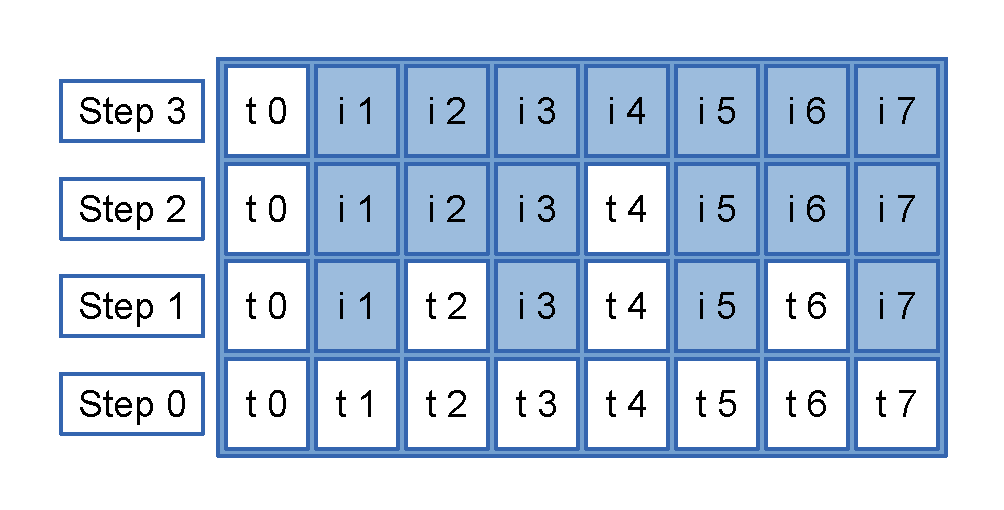
\includegraphics[width=120mm]{cudareduction.pdf}
\caption{\gls{CUDA} reduction}
\label{cudareduction}
\end{figure}

Reduction is done by halving a number of threads repeatedly and finding the lowest of two values. Each time a thread compares two value and stores the value and index of the lowest one, the number of threads active for the next step is halved. This continues until only one thread remains. However, due to the way \gls{CUDA} works, there is limited support for global synchronization across all threads in all blocks. Synchronization is required to make sure that no thread is on another "step" than the rest of the threads. If a thread was to get ahead of the rest of the threads, this would cause incorrect results, as it would try to use values that are not yet ready. In order to  guarantee correctness, the reduction is therefore done in two separate \gls{CUDA} calls, or steps. The first step reduces the number of values to be minimized significantly (using multiple blocks of threads), and the second step will reduce it to one single value (using a single block of threads). 


Each value of the Qxy-matrix can be considered a measurement of how low the error is while having the emitter in this location. The location is given by the indexes of the matrix, which reflects the position in the grid used for \gls{NLLS}. When reducing the matrix, the index of the lowest value has to be kept, as this indicates the most likely location of the emitter. Normally, a simple "find the minimum reduction" would return only the value, but in this case, the original index of the lowest value is required. While the reduction takes place, the original index in the Qxy-matrix is also kept.

It might be tempting to do the reduction, only keeping the index and not the values, and using the index to look up the values as required. As the reduction is carried out, the step between each value of interest in the original Qxy-matrix becomes large. This can lead to poor performance, as cache-misses would be very common. Bringing not only the original Qxy-matrix index, but also the associated value resolves this. Some time was spent optimizing this implementation, but focus was on correctness, rather than perfect speedup. One potential area for future improvement is memory access patterns, including better use of low latency/high speed memory \cite{harris2007optimizing}. 


\newpage


\section{\Glsentrylong{GA}}
\subsection{Overview}

\begin{figure}[htp]
\centering
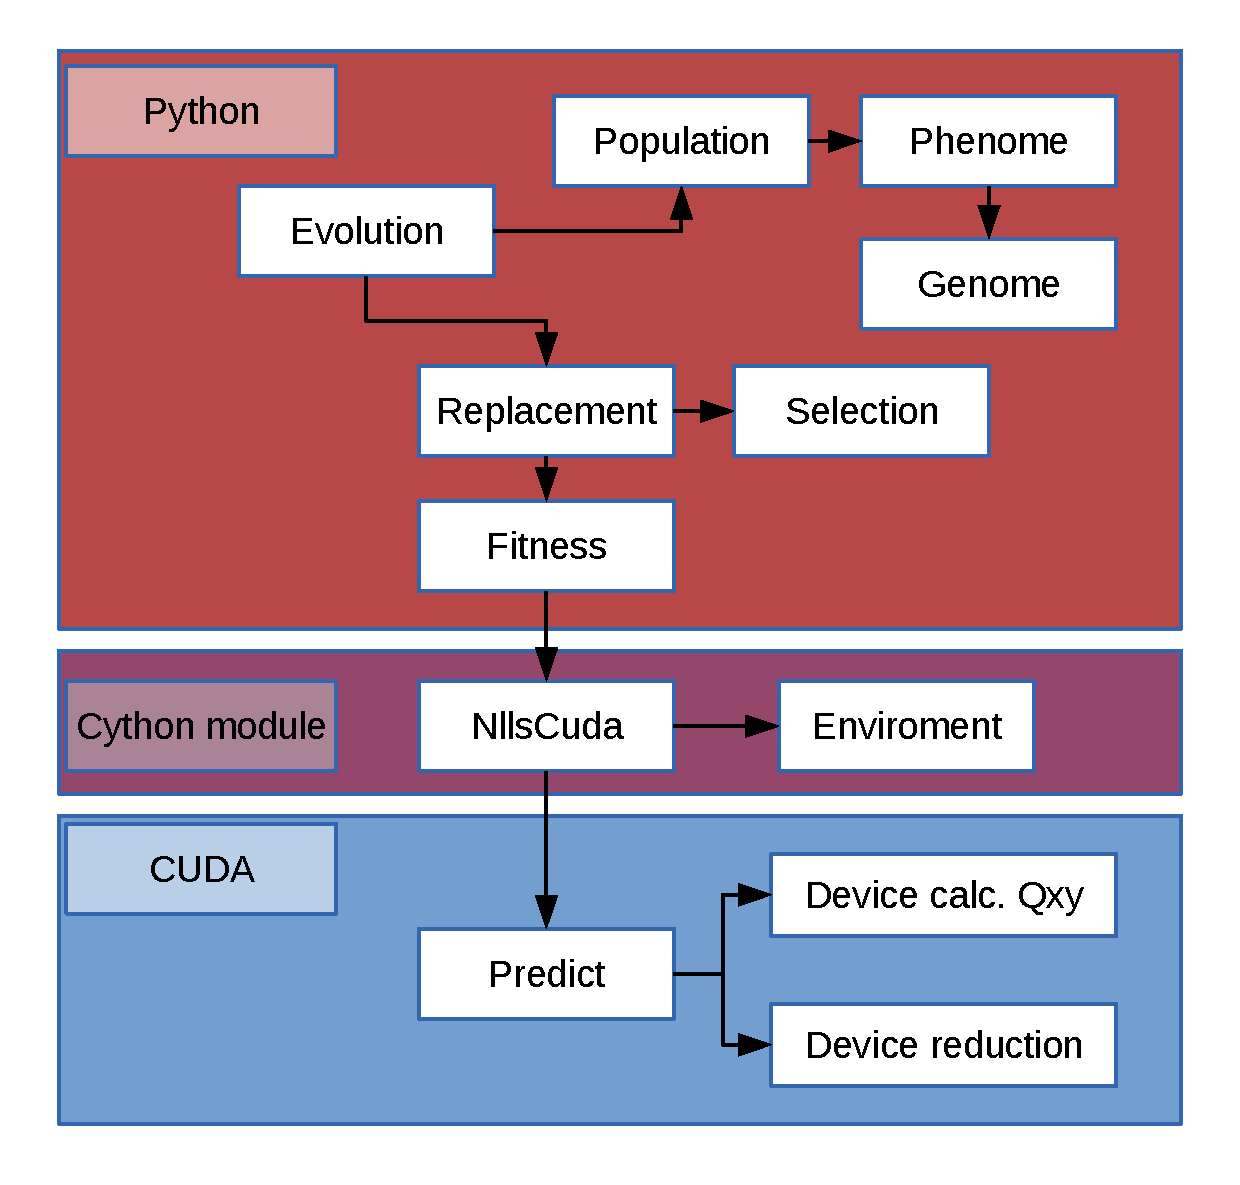
\includegraphics[width=90mm]{Codeoverview.pdf}
\caption{Overview of code}
\label{overviewofcode}
\end{figure}

The implemented code is separated into three parts: a \gls{GA} implementation in Python, a simulation and fitness-evaluation module in Cython, and an \gls{NLLS} \gls{PDOA} implementation in \gls{CUDA} (C++). This was done in order to achieve sufficient performance, for testing configurations with more than a couple of receivers. \gls{NLLS}, the \gls{PDOA} algorithm used, scales as $O(N \cdot M \cdot D^2)$. $N$ and $M$ is the steps in the grid used, and $D$ is the number of receivers. Increasing the number of receivers from 3 to 4 increases the required computational effort by a factor of $1.8$. Doubling the grid size or cutting the step size in each direction of the grid by a factor of 2 would increase the computational effort by a factor of $4.0$. 

\newpage 
In this work, a real-coded \gls{GA} was implemented. A problem-solving \gls{GA} is composed of both general and problem-specific parts. The general parts of a \gls{GA} include:

\begin{itemize}
\item Selection methods - used to select which genomes are allowed to reproduce and pass on genes.
\item Replacement strategy - defines how the new generation is created from the parent generation
\item Population manager - a container for a group of phenomes
\end{itemize}

These parts of a \gls{GA}-implementation are usually general, and do not contain any problem-specific knowledge. Defining the best selection method and replacement strategy is an area where a considerable amount of research has been conducted \cite{goldberg1988genetic}. The result of this research are several methods for both selection and replacement, which each have their strong and weak properties. Selection methods are important, as they define what is known as the selection pressure. The selection pressure is a measure of how hard it is for phenomes to pass down genes. A very high selection pressure leads to a quickly diminishing variance in the population, resulting in a very narrow search in the search space. Some examples of selection methods are:

\begin{itemize}
\item Roulette selection - borrows features from a roulette, where a greater area of the roulette is given to the individual with the highest (best) fitness.
\item Sigma scaling selection - extension of the roulette selection that uses scaling of the raw fitness values to make a less drastic difference between the best and the worst phenome of the population, effectively reducing selection pressure.
\item Boltzmann scaling selection - scaling that implements a temperature measure in order to avoid selecting a local optima early on, and to keep the selection pressure up during later generations.
\item Rank scaling selection - scaling where the relation between the individuals is considered. This reduces selection pressure, as fitness is set based on individuals' relation/rank in the population, rather than some variation on its fitness.
\end{itemize}

During this work, all of the above selection strategies were implemented. Attempting different combinations of replacement and selection strategies lead to using rank scaling selection to lessen the selection pressure. The selection pressure initially is often high, as one individual can easily overcome all the others that are still have a poor fitness.

The replacement strategy selected also plays a role in the selection pressure. When moving from one generation to the next, the replacement strategy will define how the transformation between the old (parent) generation to the new (children) generation is done. Some replacement strategies include:

\begin{itemize}
\item Full generation replacement - creating a new population based on the given selection method; the new population is the same size as the old one.
\item Over-production replacement - replacing the old generation of $N$ individuals by creating a new population of $N+M$ individuals ($M > 0$). From the new population, $N$ of the $N+M$ is selected to form the next generation.
\item Generational mixing replacement - creating a new generation based on the old generation, and then combining this with the old generation, effectively making the new generation and the old generation compete to be included in the next generation.
\end{itemize}

Several replacement strategies, as mentioned above, were also implemented. For this work, I ended up using a full generation replacement combined with elitism. The number of old individuals kept was usually set to two. This is similar to a generational-mixing replacement strategy, but has less selection pressure. Only two individuals from the old generation are included, as opposed to including the entire old generation and making old and new generations compete.




\subsection{Genome and phenome - Step 2 and 4}
\label{GP}

Two different types of encoding were used for the genome:

\begin{enumerate}
\item Cartesian coordinates
\item Polar coordinates
\end{enumerate}

Cartesian coordinates is a genome implementation where each coordinate is given a real value. A genome consist of an array of $2N$ floating numbers, where N is the number of receivers in the configuration. In addition, all genomes in a single run will share a base position. Their coordinates can be considered offsets from this base position.

Likewise, polar coordinates are encoded using two real numbers; an angle ($\theta$) and a radius (r). Each of these are a floating number. The genome therefore contains $2N$ floating numbers. Polar coordinate genome also uses a base position.

Cartesian coordinates offer an encoding that gives an intuitive world view for the search, however, it does not handle rotation or relocation as gracefully as polar coordinate encoding. Using polar coordinates allows for easier manipulation of the configuration in particular rotation and relocation. These are useful properties in regard to problem 2 (Subsection \ref{P2RPC}).


\subsection{Genome and phenome - Step 3}
\label{EAGENOMEPATH}

In Step 3, a concept of a path, or a set of waypoints for each \gls{UAV}, is introduced. This is reflected in the genome-encoding, using a variant of the NASA-antenna encoding \cite{hornby2006automated}. The NASA-antenna encoding is a recursive encoding, effectively giving a tree-like structure. For the purpose of encoding a \gls{UAV} path, only a single branch per \gls{UAV} is required. The encoding can therefore be flattened to a list of angles. This is best illustrated in Figure \ref{genomestep3}, showing an example using only one \gls{UAV} and the path for this \gls{UAV}. 

\begin{figure}[htp]
\centering
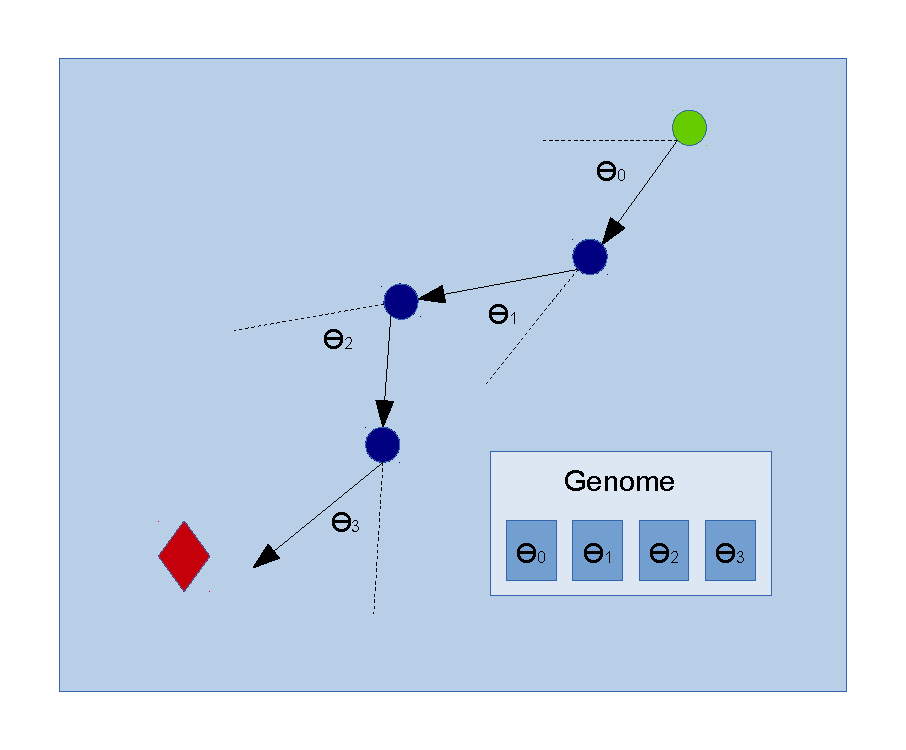
\includegraphics[width=90mm]{eaencodingstep3.pdf}
\caption{Genome - Step 3}
\label{genomestep3}
\end{figure}

The first angle ($\theta_0$) is defined as an offset compared to a predefined fixed axis; for instance, the X-axis as seen in Figure \ref{genomestep3}. Further direction-changes are then defined as offsets compared to the current heading of the \gls{UAV}. This method of encoding allows the genome to optimize the general direction of the path just by changing the initial angles. Since the path is specified relative to previous steps in the path, the behaviour will be replicated in the new direction. 

Extending this encoding to multiple \glspl{UAV} is trivial. The list of angles for one \gls{UAV} is replicated for each of the N \glspl{UAV}. Effectively, the genome size then becomes $N*M$, where $N$ is the number of \glspl{UAV} and $M$ is the number of steps per \gls{UAV}. It is important to note that, in this encoding there is no way for the \gls{GA} to change the length of a step. The step length is considered fixed; this comes from an assumption of a fixed travelling speed and a given fixed sample rate. 

The phenome consists of a set of points in space, rather than the abstract list of angles. Interpreting/developing the genome to a phenome is done by applying the rules, as specified previously in this section, and returning a list of coordinates that can be evaluated using the fitness-function (Subsection \ref{MFS3}). 

\subsection{Crossover}
\label{EACROSSOVER}
Crossover was implemented as a standard, single-point crossover. In cases where the representation required it, it was done by making a linear sequence of the genome. For the Cartesian and Polar genome, each genome consists of a set of receivers-locations. Each receiver-location consists of a set of coordinates. By reducing this list of lists to single list of floats, a single point crossover can be performed as normal:

\begin{enumerate}
\item Select an \texttt{INDEX} equal or greater than 0 and less than the "length of the lists"
\item Split serial lists of receivers in two parts, from 0 to \texttt{INDEX}, and from \texttt{INDEX} to "length of the lists".
\item Take the first part of each of the list and append this to two new lists.
\item Take the second part of the two lists, append them to each of the new lists, so that the new lists have one part from each parent
\end{enumerate}

A single-point crossover is used for all genome representations, and works in a similar way in all three cases. The effect that a crossover has differs between the three different representations.

For a Cartesian coordinate genome, a receiver-position may be split between X and Y coordinate, resulting in the corresponding receiver in the new genome being a combination of two receivers. This will keep vertical or horizontal displacement, but cause a (potentially) large jump along the other axis. 

For Polar coordinates, the process could cause the angle ($\theta$) from one receiver to be combined with the radius (r) from another. The result is that the new receiver would do a similarly large jump in either angle or radius. 

Using the Path genome  (Subsection \ref{EAGENOMEPATH}), a split could occur in the middle of the sequence of angles describing the path of a \gls{UAV}. The effect of this would be that the \gls{UAV} in question would get the first part of the path from one individual, while the second part would originate from the other. As the direction of the path is defined relative to previous steps, a change in the initial angles could change the direction of the entire path.

\subsection{Mutation}
\label{EAMUTATION}
Mutation should, most often, provide a small change in some of the parameters of the solution, in order to improve the solution. It should normally not result in a large jump in the search space. In order to achieve this, the following solution was applied for each parameter:
\begin{enumerate}
\item Draw a uniformly distributed random number, less than 100
\item If the random number is greater than a given percentage (default: 5), the parameter will not be mutated.
\item Otherwise, mutate the parameter by adding or subtracting a small value
\end{enumerate}

Which value is added or subtracted when mutation occurs is random, however, care was taken to make sure that only applicable actions/mutations are possible. There are several special cases to consider. These occur when:

\begin{itemize}
\item Cartesian coordinates: when bordering the defined maximum and minimum area
\item Polar coordinates: when on the edge of the maximum radius or minimum radius
\item Polar coordinates: when a full rotation has occurred ($\theta > 2\pi$)
\item Path genome: when a full rotation has occurred ($\theta > 2\pi$)
\end{itemize}

For all of the cases above where a mutation would lead to a coordinate (Cartesian or radius) being out of the predefined area, the given coordinate is locked to the boundary.

\begin{equation}
X_{new} = \max{(X_{min},\min{(X_{max},X_{old})})} \nonumber
\end{equation}

This is the general method for constraint-handling used throughout the implementation. If the value, as given by the real-coded \gls{GA}, is outside the bounded area, it will be clamped to the border of the area. 

Any full rotations that might occur for Polar coordinate genome or Path genome are handled by adding or subtracting $2\pi$ (normalizing the angle), depending on the direction of the rotation. This is not strictly necessary, but is done for consistency.

\subsection{Fitness - Step 4}
\label{MFS4}
Fitness is defined as the average error of the location predictions. The actual emitter-location is used as the reference point. This leads to the following formula for fitness of a configuration:

\begin{eqnarray}
\boldsymbol{d}_\text{i} &=& \boldsymbol{x}_\text{pred,i} - \boldsymbol{x}_\text{em}\nonumber\\
d_\text{avg} &=& \sqrt{\cfrac{1}{n}\sum_{i=0}^{n}{||\boldsymbol{d}_\text{i}}||^2} \nonumber\\
F &=& 100 - K * d_\text{avg}\nonumber
\end{eqnarray}

$\boldsymbol{x}_\text{pred,i}$ is the coordinates of a location prediction $i$ by the \gls{PDOA} algorithm. $\boldsymbol{x}_\text{em}$ is the actual location of the emitter. $\boldsymbol{d}_\text{i}$ is the deviation of prediction $i$ from the actual emitter-location. $d_\text{avg}$ is the average prediction error from the actual emitter-location. $F$ is the fitness value. $K$ is a constant used to scale the fitness value between $0$ and $100$.

The fitness-function, as described, is the simplest possible means of comparing two sets of predictions in regards to their deviation from the exact answer. It will only consider the absolute deviation in distance. This makes a set of predictions spread around the emitter in a circle with radius $R$. These are indistinguishable from a set of predictions in a single point at a distance $R$ from the emitter. 

Implementing a fitness-function that better handles the complex distribution of the predictions, could be done using \glspl{FMM}. \Glspl{FMM} can estimate the distribution of the predictions and enable the fitness-function to consider not only the deviation of each prediction, but more extensive characteristics, such as the spread or variance of the predictions. Implementing this would add another computationally intensive operation to each fitness-evaluation (estimating the distribution). Preliminary tests, using \gls{FMM} as part of an automated evaluation process, showed that \gls{FMM}-generated models may behave erratically with limited data. Making a robust fitness-function utilizing \gls{FMM} is, for this reason, considered future work.

\newpage
\subsection{Fitness - Step 3}
\label{MFS3}

%todo review this section

The fitness-function for evaluating the performance of a set of paths is similar to that of a set of points from Subsection \ref{MFS4}. In addition to average error, a concept of a bias ($\boldsymbol{b}$) and variance ($\sigma^2$) is introduced. $\boldsymbol{b}$ is the mean error of the predictions. Generally, it is better if the $||\boldsymbol{b}||$ is close to $0$. The spread of the predictions are not taken into account yet.

\begin{eqnarray}
\boldsymbol{x}_\text{avg} &=& \cfrac{1}{n} \sum_{i=0}^{n} \boldsymbol{x}_\text{pred,i}\nonumber \\
\boldsymbol{b} &=& \boldsymbol{x}_\text{avg} - \boldsymbol{x}_\text{em} \nonumber 
\end{eqnarray}


Variance gives a measure of the spread of the predictions generated. In order to not penalize formations that have a skewed mean ($||\boldsymbol{b}|| \neq 0$), this variance ($\sigma^2$) is calculated relative to the average position predicted ($\boldsymbol{x}_\text{avg}$).  $\boldsymbol{\epsilon}_\text{i}$ is the error of prediction $i$, relative to the average predicted location ($\boldsymbol{x}_\text{avg}$) 


\begin{eqnarray}
\boldsymbol{\epsilon}_\text{i} &=& \boldsymbol{x}_\text{pred,i} - \boldsymbol{x}_\text{avg} \nonumber \\
\sigma^2 &=& \cfrac{1}{n} \sum_{i=0}^{n} ||\boldsymbol{\epsilon}_\text{i} || ^2 \nonumber
\end{eqnarray}

Combining the variance and average error to form a fitness-measure is non-trivial, as it is beneficial to scale the fitness-value ($F$) to between certain values. In the \gls{GA}-implementation used for this work, fitness ($F$) is assumed to be a value between $0$ and $100$. The solution developed involves a scaling that differentiates strongly between good solutions, and has less numerical difference for bad solutions.


\begin{eqnarray}
F &=& \cfrac{100.0}{1.0 + K * \sigma^2 * d_\text{avg}} \nonumber
\end{eqnarray}

The constant $K$ is defined as a number $0.0 < K < 1.0$. $K$ is set as to allow the really good solutions, for many \glspl{UAV} and steps, to get a fitness value ($F$) close to $100$. $d_\text{avg}$ is the same as used for Fitness - Step 4 (Subsection \ref{MFS4}). Solutions with few resources may be as low as $1.0-3.0$ in fitness value ($F$) when fully optimized by the \gls{GA}.



\newpage

\subsection{Fitness - Step 2}
\label{MFS2}

%todo reread this section

In the initial phases of the search, the receivers/\glspl{UAV} are far away from the emitter. In this state, a rough estimate of the location of the emitter is required to know in which general direction to proceed. In this setting, the receivers were restricted to a small area, a certain distance from the emitter. Initially, solutions were tested against a fixed emitter, causing the formations to become directionally dependant. This is an unfavourable trait, as the receivers have no idea of the whereabouts of the emitter in this state, and would not be able to direct themselves in the direction of the emitter. To counter this, a configuration could be rotated in order to simulate the emitter being in different directions, in relation to the receiver-configuration. 

Changing the perceived direction of the emitter can be done simply by rotating the formation. Polar coordinates make this operation trivial. Evaluating the fitness of a receiver configuration is done as following:

\begin{enumerate}
\item Calculate the average error (in predictions) for the configuration using an angle-offset ($d\theta$), which is added to each of the angles specified in Polar coordinate genome.
\item Add the average error to the list of results.
\item Select the next offset and go back to 1. If there are no more offsets, continue.
\item Calculate the fitness using the average of the values in the result list
\end{enumerate}

Fitness-value ($F$) in Step 2 is calculated in the same way as for Step 4 (Subsection \ref{MFS4}).
The distance from the center-point of the configuration (the pole of the polar coordinates) to the emitter, is considered fixed for a \gls{GA} run. Implementation does, however, allow the center-point of the configuration to be freely specified, should it be required.


\newpage


\section{\Glsentrylong{MOEA}}

\subsection{Overview}

\begin{figure}[htp]
\centering
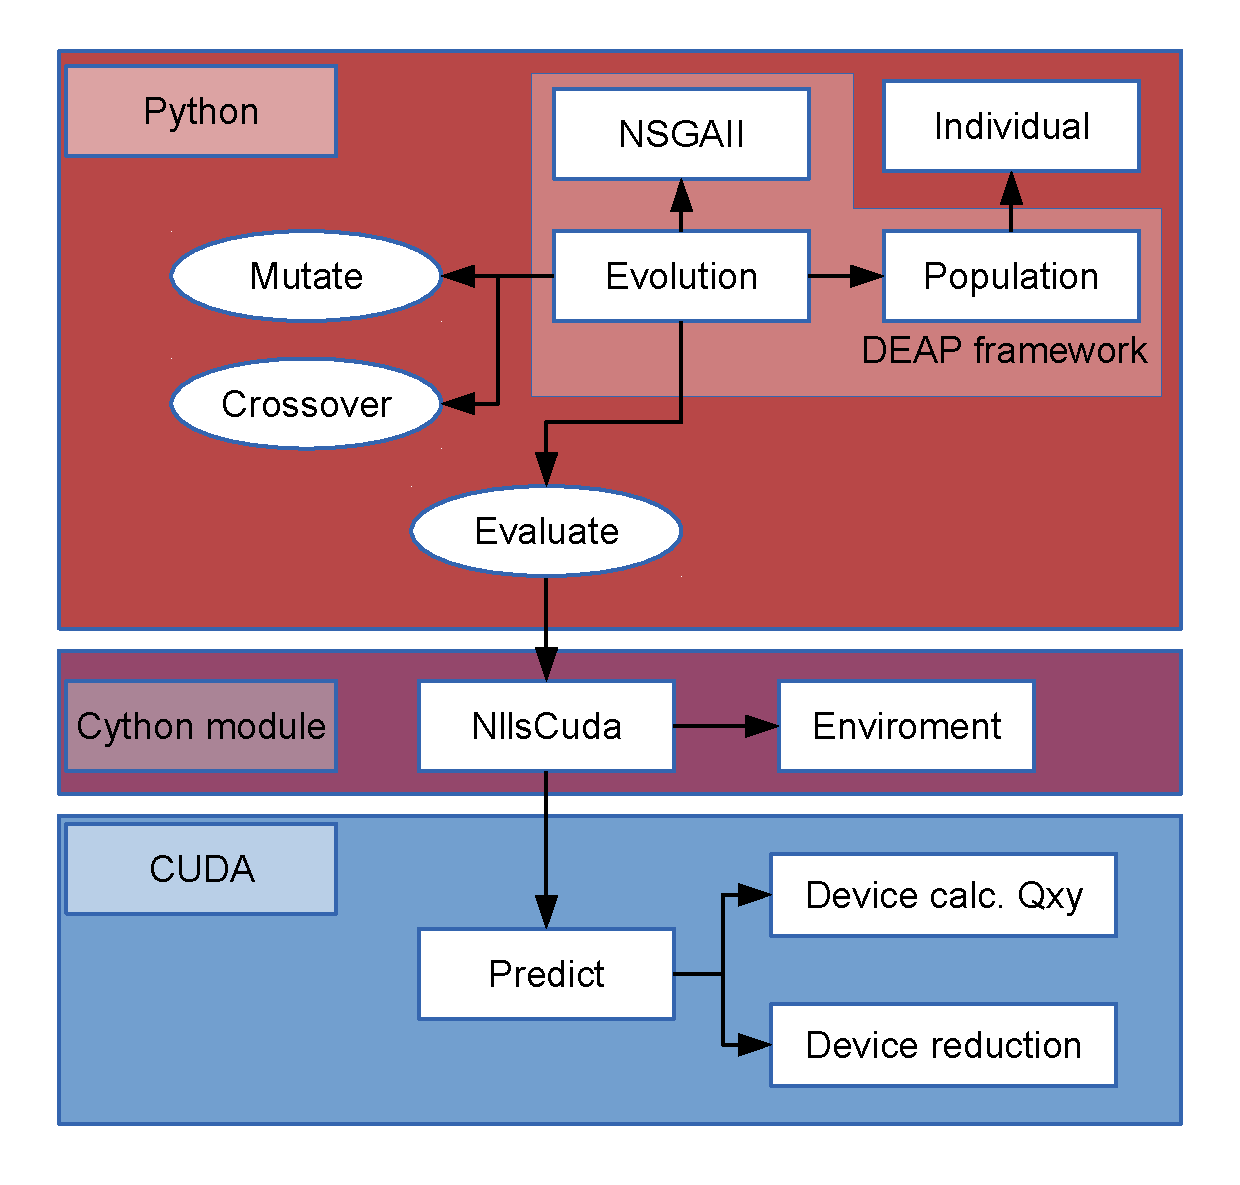
\includegraphics[width=90mm]{Moeaoverview.pdf}
\caption{Overview of \acrfull{MOEA}}
\label{overviewofmoea}
\end{figure}


The \gls{MOEA} borrows from the single-objective \gls{GA} optimization, and uses the same back-end for fitness-evaluation. Most of the higher-level code from the \gls{GA} has been replaced by specially tailored functions, in addition to the Python DEAP framework \cite{DEAP_JMLR2012}. The framework handles selection and implements NSGAII. Problem-specific knowledge for the individual encoding, mutation, crossover and evaluation was implemented and is described in the following subsections. 

%TODO CITE NSGAII

Three different multi-objective scenarios were explored:

\begin{enumerate}
\item Variance vs average error
\item \gls{UAV} count vs average error
\item Step length vs average error
\end{enumerate}

Variance vs average error is a result of previous work, where formations appeared that seemed to predicted mean-value correctly, but had a large spread. In an effort to improve on this, a contribution from the variance of the predictions is included in the \gls{GA} fitness-evaluation. Using the variance, as well as the average error, proved to be problematic in regard to fitness-scaling and normalization. Improving this could be done by trying to use a different method of combining variance and average error to one fitness-value (instead of multiplying the two factors, as in Subsection \ref{MFS3}). One possibility would be to introduce a weighting of the two components. In order to get a better impression about what the weights could be, the variance vs average error \gls{MOEA}-scenario was devised.

\gls{UAV} count vs average error was conceived as a way to describe, not only the best configuration for $N$ \glspl{UAV}, but also develop a good formation using $N-1$ \glspl{UAV}. A single-objective \gls{GA}, generates a set of highly specialized solutions, given a single selection criterion. Moderate variance in results from the single-objective \gls{GA}, along with highly specialized solutions, made it difficult to compare results between runs. Optimizing both average error and \gls{UAV}-count at the same time allows the solution for $N$ \glspl{UAV} to inherit features from the solution for $N-1$ \glspl{UAV}. The relation between the different solutions can be used to better evaluate the effect of adding another \gls{UAV}, and is also able to say something about the change in strategy, should a \gls{UAV} be removed from the pool. 

The way the encoding is structured for the \gls{GA}, it is not possible for a \gls{UAV} to stand still at the same spot. This is a restriction that may or may not be realistic; quad-copters, for instance, are perfectly able to stand still in one spot while gathering data. Introducing a variable step length means increasing the search space, and with it, the computational effort required to find good solutions. With this scenario, the intention was to explore how the \glspl{UAV} would use the new freedom, in being able to stand still or, alternatively, move at a lower speed.

For the \gls{MOEA}, one encoding was used for all of the different optimization-scenarios. This means that for each of the scenarios, certain parts of the genome was inactive and locked. Locking part of the genome was done to reduce the search space, focusing the computational effort where it was more useful.

\newpage


\subsection{Genetic encoding}


\begin{figure}[htp]
\centering
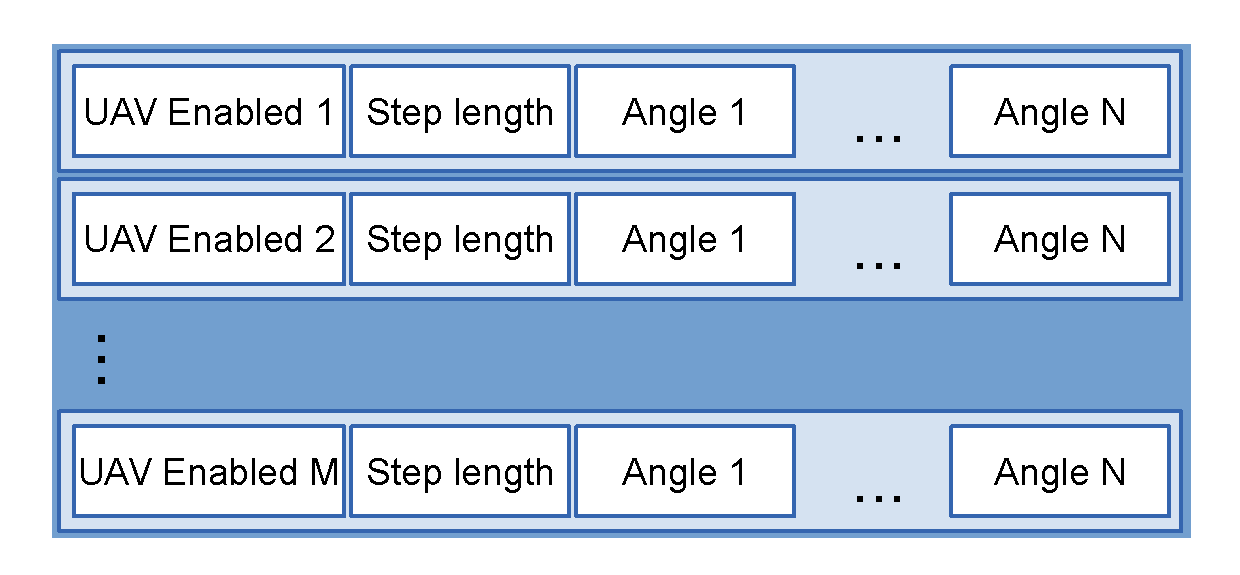
\includegraphics[width=90mm]{Moeaencoding.pdf}
\caption{Genetic encoding for \gls{MOEA}}
\label{encodingmoea}
\end{figure}

The genetic encoding for the \gls{MOEA} is implemented as a list consisting mostly of real numbers. A general structure of this list can be seen in Figure \ref{encodingmoea}. For each \gls{UAV}, there is a set of parameters consisting of: "\gls{UAV} Enabled", "Step length" and angles. Within a single optimization run, the size of the genome will remain constant. It is possible to configure for optimization of any number of \glspl{UAV} and steps. As a result, the size of the genome will vary between different runs of the \gls{MOEA}. 

\Gls{MOEA} implements a distinction between genotype and phenotype by a separate pre-evaluation step. This step converts the genome to a set of attributes which can be evaluated. For each evaluation of an individual, the following values are calculated: 

\begin{enumerate}
\item Maximal distance travelled by one of the \glspl{UAV}
\item The number of active \glspl{UAV}
\item The average error and variance of the predictions generated
\end{enumerate}

The maximum distance travelled by one of the \glspl{UAV} is calculated by iterating over the \glspl{UAV} in the individual, and finding the highest step length. The step length is then multiplied by the number of steps in total to find the distance travelled. For the number of active \glspl{UAV}, the value found under each of the "\gls{UAV} Enabled" genes are summed. An active/enabled \gls{UAV} will have this value set to 1, while an inactive \gls{UAV} will be 0.

For more information about how the average error and variance is calculated, refer to Subsection \ref{MFS4} and \ref{MFS3}. The same approach is used, however, the raw average error and variance-values are used instead of the fitness-value.



\newpage
\subsection{Crossover and mutation}

As crossover-operator, a modified single-point crossover is used. There were some issues in regard to doing crossover between two individuals, resulting in a new individual with no active \glspl{UAV}. To solve this problem, a new crossover-index will be selected until a suitable crossover-point is found. If it is not possible to find a crossover that results in \textit{both} new individuals having at least one active \gls{UAV}, the individuals will not be crossed. 

When the mutation-operator is called, it is assumed that a mutation has to happen (i.e the mutation probability is already accounted for). Choosing the gene to be mutated is done as following:

\begin{itemize}
\item (Optional) If the "UAV Enabled"-parameter is not locked, there is a 50/50 chance that a \gls{UAV} will be turned on or off. If a \gls{UAV} is turned on or off, a mutation has occurred and the operator exits.
\item (Optional) If the "Step length"-parameter is not locked, there is a 50/50 chance that mutation will modify the step length of a \gls{UAV}. The step length is modified by adding or subtracting a random value from a Gaussian distribution. If a step length is modified, a mutation has occurred and the mutation operator exits.
\item A random angle from a random \gls{UAV} is selected for mutation. The angle is selected uniformly from the angles of the \glspl{UAV} in the individual. Mutation is applied by adding a random Gaussian-distributed value to the angle. Gaussian distribution makes large mutation-steps possible, but not very likely.  
\end{itemize}

Based on the mutation, as described above, there is an equal chance that either a step or "\gls{UAV} Enabled" gene is mutated. This effect is a result of the locking of either the "UAV Enabled" or "Step length" genes, depending on if the scenario is optimization of \gls{UAV}-count or step length. 




\newpage

\section{Interactive simulation}

\subsection{Overview}

Early in the process, it was clear that many of these problems are hard to analyse, and solutions hard to verify without resolving to a simulated environment. Similarly, it was equally challenging to get a good impression of the dynamics of the problem with long iteration times and in a fairly strict, defined scenario. To alleviate some of the issues, an interactive simulation was developed, allowing for easy testing and verification of results from the evolutionary algorithms. This framework allows the user to move around samples and see the results more-or-less instantaneously. 

There are three main features/modes to the interactive simulator developed:

\begin{enumerate}
\item Verification mode
\item Interactive mode
\item Heuristics mode
\end{enumerate}


Verification mode works as a testing ground for the formations developed by the \gls{GA} and \gls{MOEA}. In this mode, it is possible to load a formation developed by either of the two optimization-algorithms and test manual modifications to this formation, as well as relocate the emitter to get an impression of robustness. Statistics are displayed in real-time as the user manipulates the formation.

This tool was developed as a way to get an intuitive feel for the problem. The interactive components are hard to capture in this report; several videos were made of this application and are included with this report. Otherwise, the videos are also available on Youtube, and links are provided in the respective sections.


\newpage
\subsection{Interactive mode}




\begin{figure}[H]
\centering
\begin{minipage}{60mm}
  \centering
	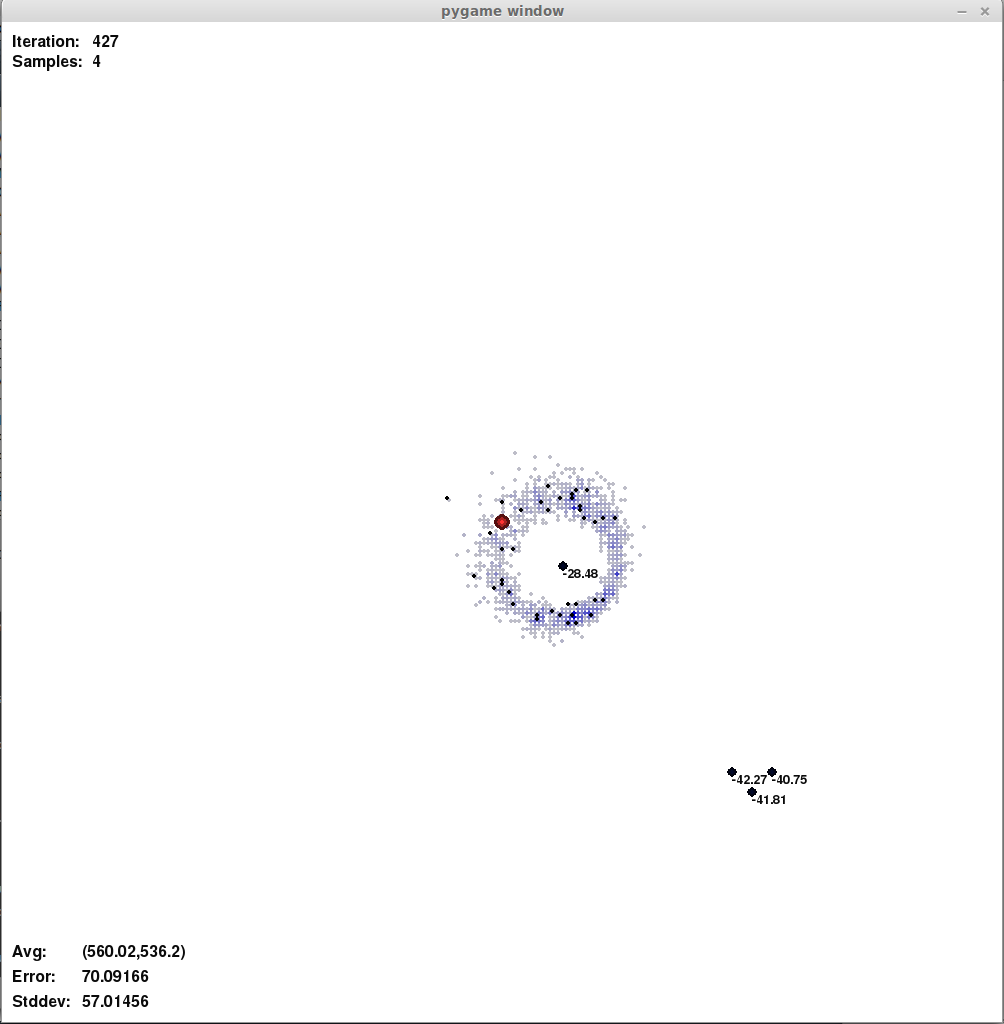
\includegraphics[width=60mm]{interactive.png}
\end{minipage}%
\begin{minipage}{60mm}
  \centering
	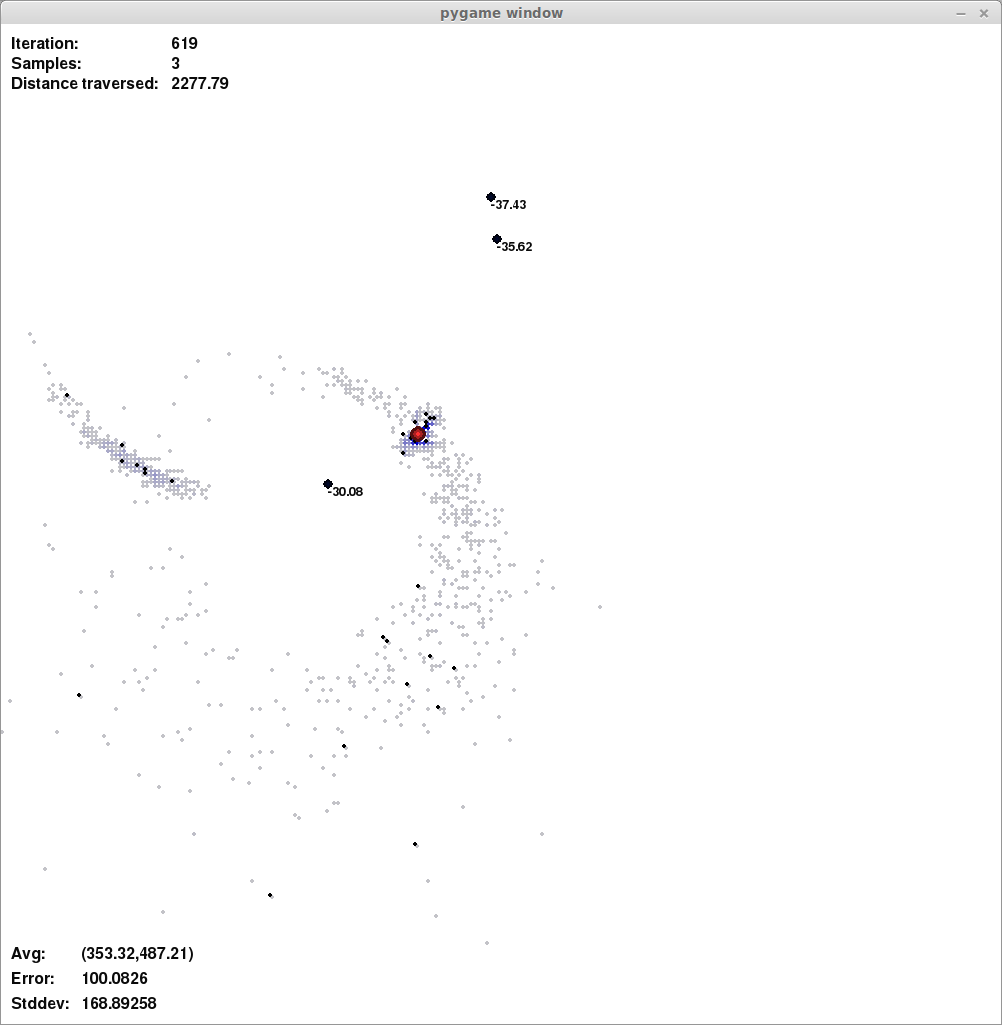
\includegraphics[width=60mm]{interactive2.png}
\end{minipage}
\begin{minipage}{60mm}
  \centering
	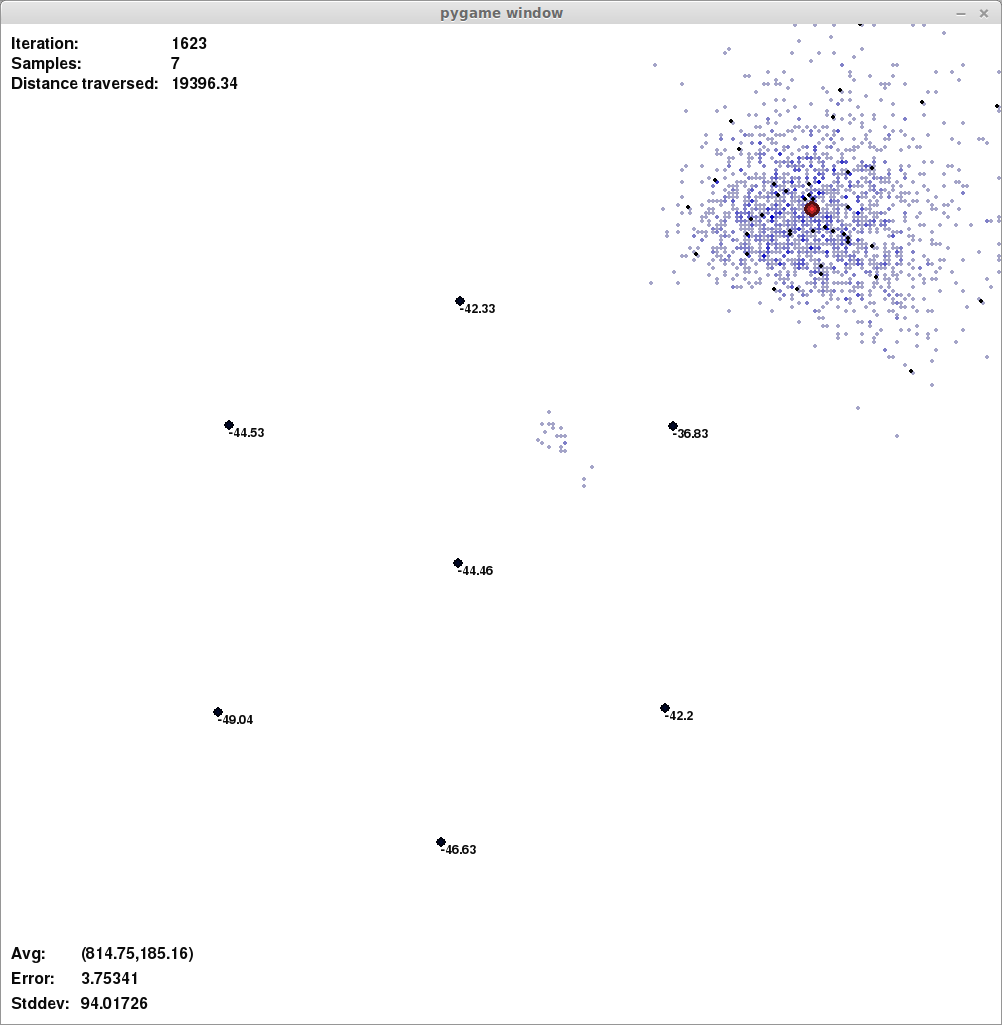
\includegraphics[width=60mm]{interactive3.png}
\end{minipage}%
\begin{minipage}{60mm}
  \centering
	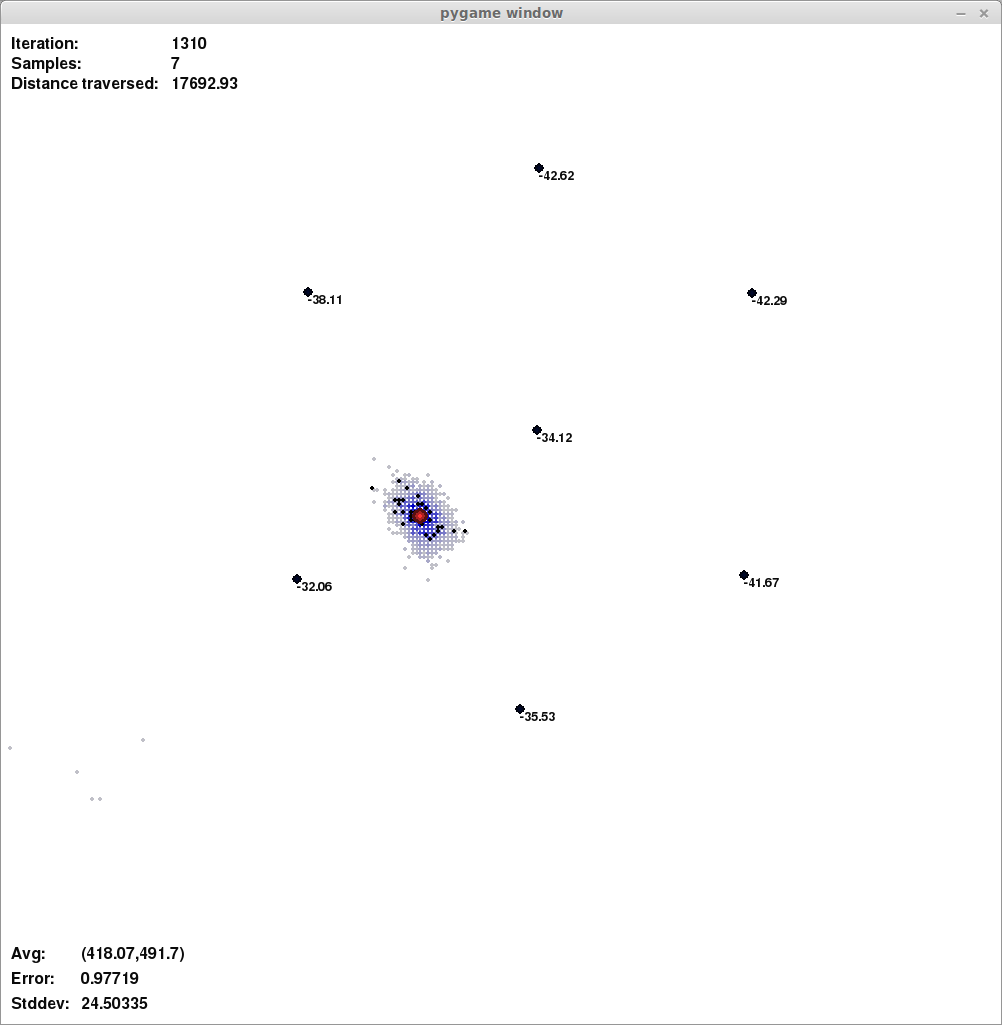
\includegraphics[width=60mm]{interactive4.png}
\end{minipage}
\caption{Simulator - Interactive mode}
\label{simulator_interactive}
\end{figure}


Interactive mode allows for manual testing of different formations to get a better intuitive impression of the dynamics at work in this problem. This proved extremely useful when trying to demonstrate the problem complexity and debugging errors in the fitness-functions.


To get a better impression of how this mode works, there is a short video of it found here: \url{http://youtu.be/i0vveyy6uZk}


\subsection{Heuristics mode}


\begin{figure}[H]
\centering
\begin{minipage}{60mm}
  \centering
	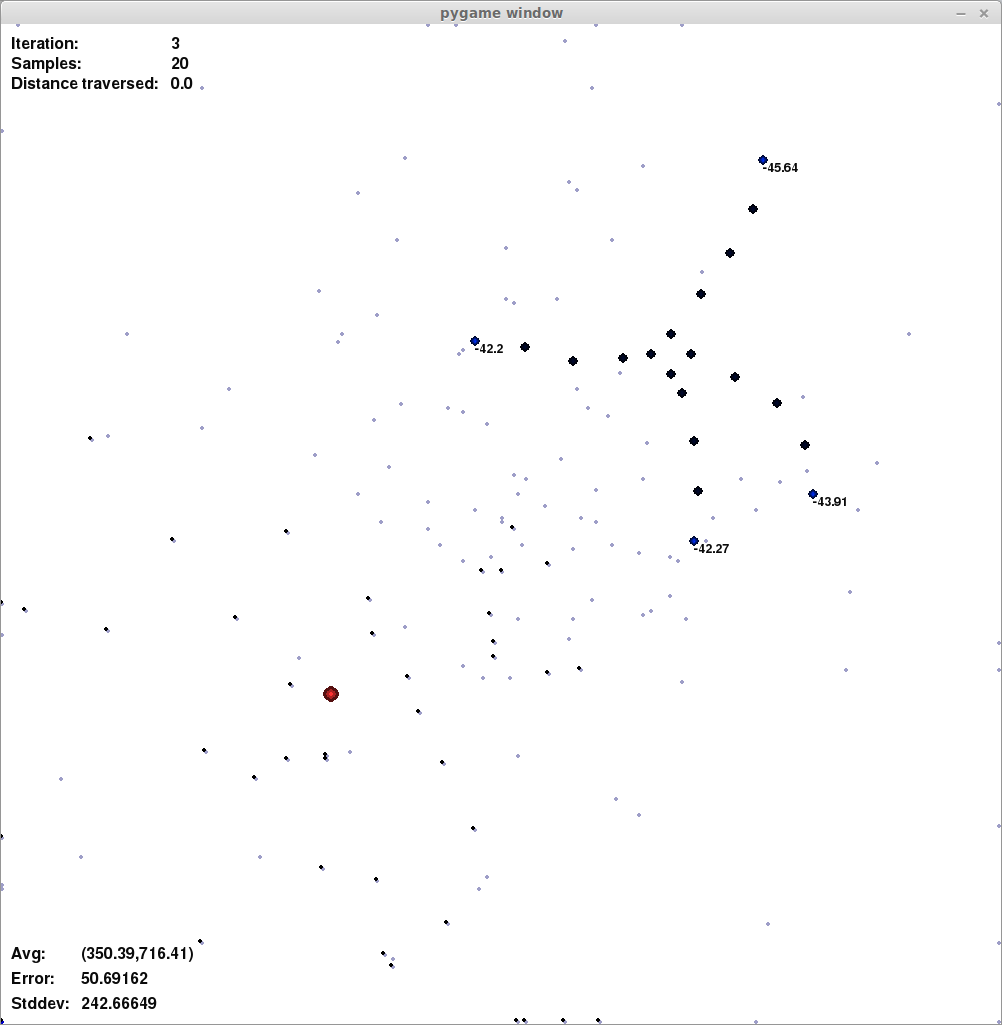
\includegraphics[width=60mm]{heuristics2.png}
	
\end{minipage}%
\begin{minipage}{60mm}
  \centering
	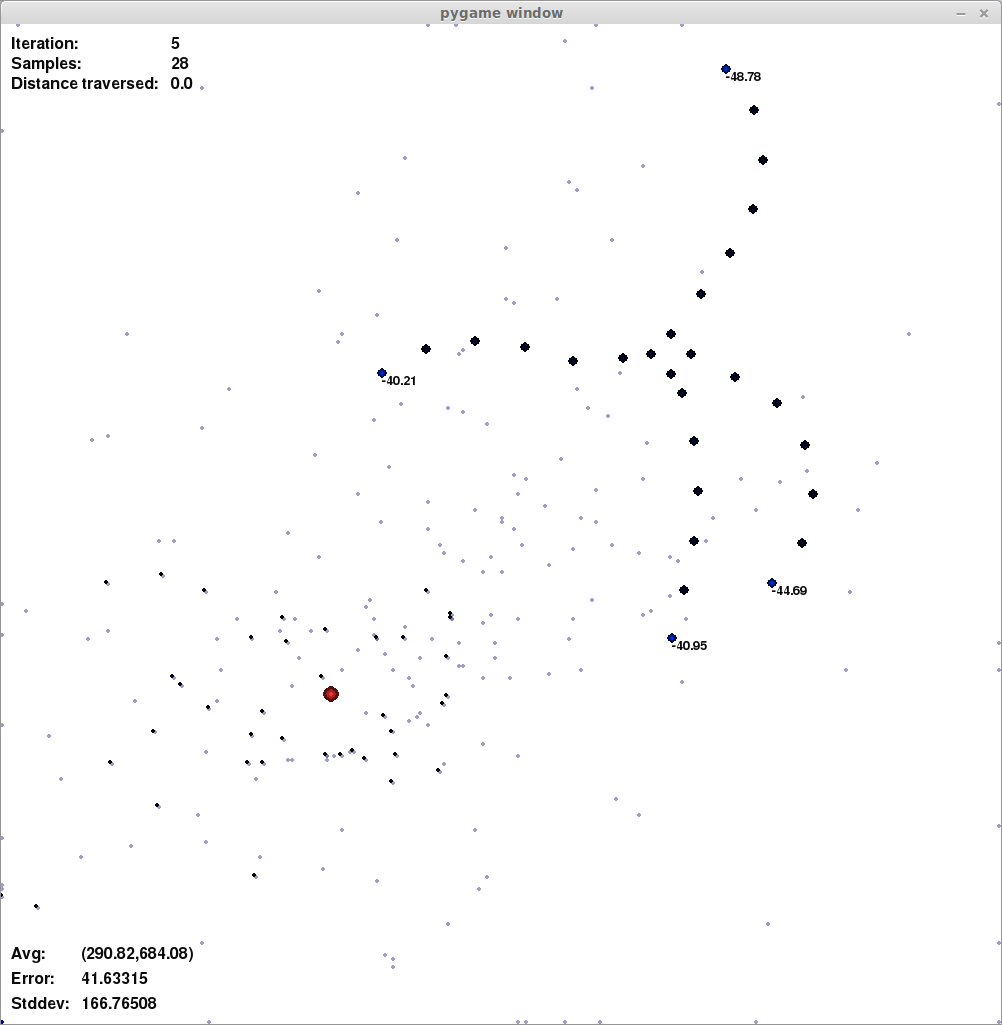
\includegraphics[width=60mm]{heuristics3.png}
\end{minipage}
\begin{minipage}{60mm}
  \centering
	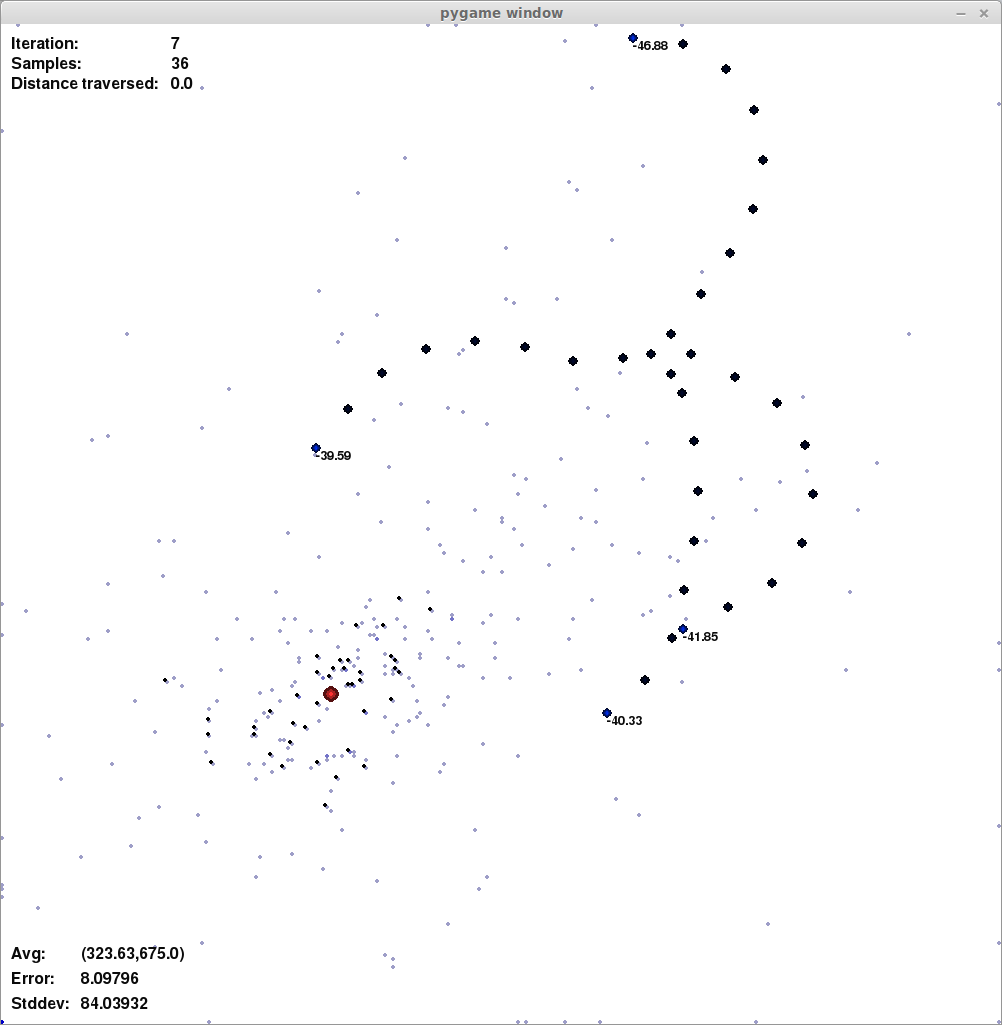
\includegraphics[width=60mm]{heuristics4.png}
\end{minipage}%
\begin{minipage}{60mm}
  \centering
	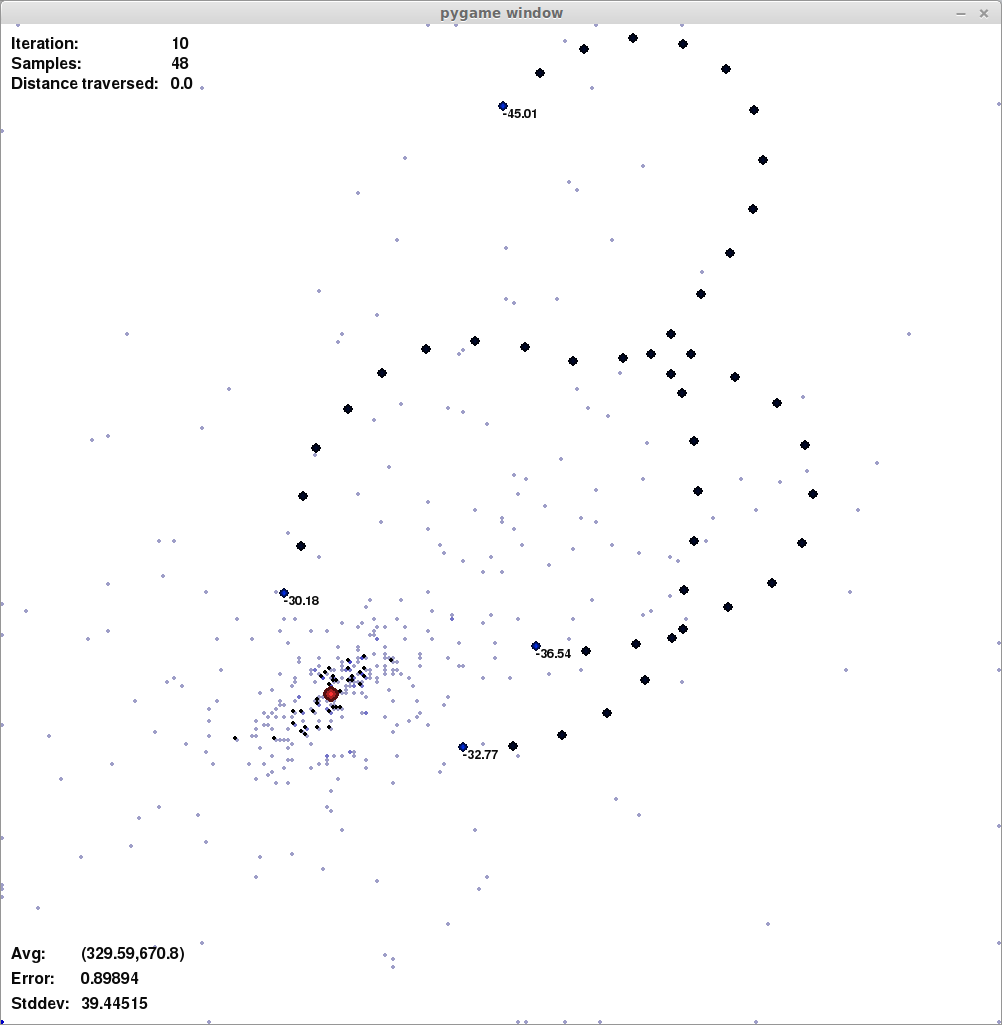
\includegraphics[width=60mm]{heuristics5.png}
\end{minipage}
\caption{Simulator - Heuristic mode}
\label{simulator_heuristics}
\end{figure}




Heuristics mode allows for batch-testing of the different heuristics developed. This can be conducted with or without a graphical user interface. The graphical user interface takes a bit of extra computational power, but gives a much better view on how the different agents/heuristics act in reaction to the information available. 


Youtube video: \url{http://youtu.be/Z_lu8-Jifno}


\subsection{\Glsentrylong{FMM}}
\label{M_INTER_FMM}


\begin{figure}[htp]
\centering
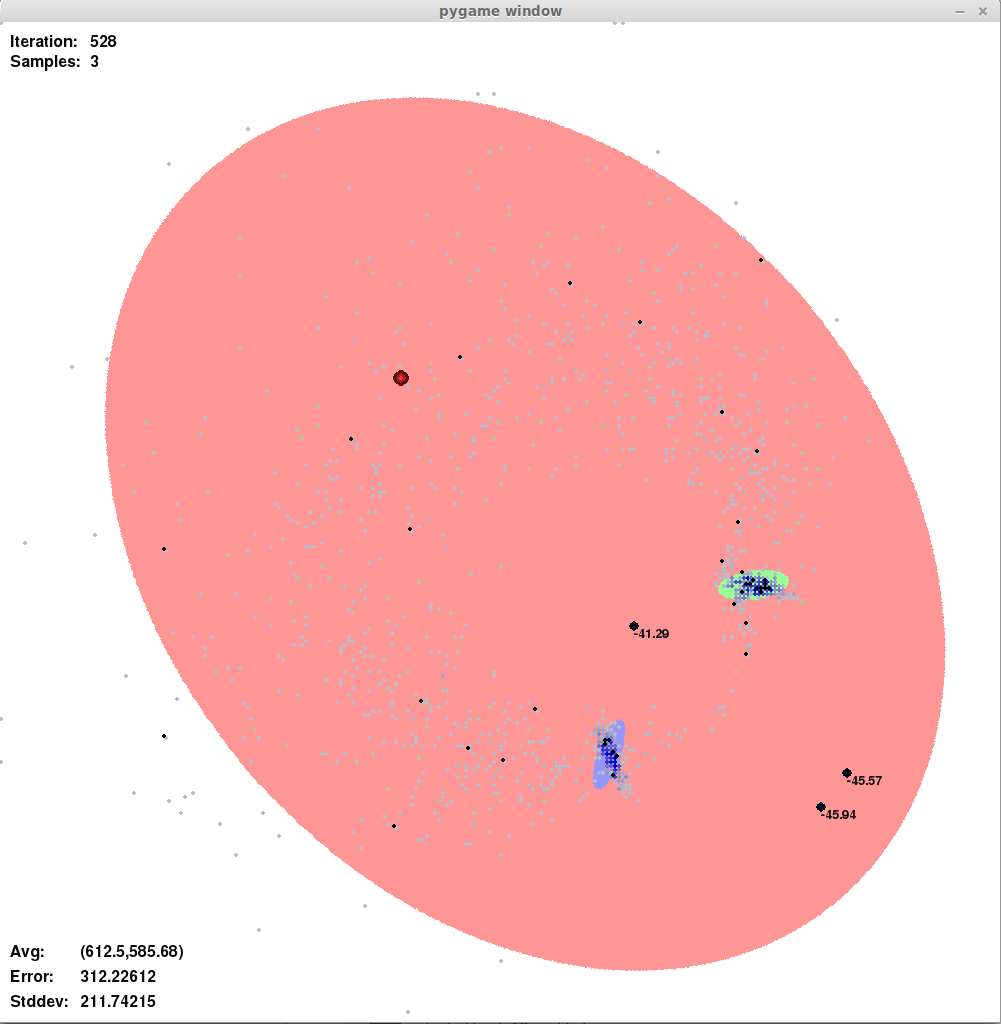
\includegraphics[width=70mm]{fmm.png}
\caption{Simulator - \gls{FMM}}
\end{figure}


\Gls{FMM} involves fitting a model, consisting of multiple, well defined probability distributions, to arbitrary data. The prospective data to be modelled using \gls{FMM} are the predictions generated through simulations. These, generally, show decent clustering, but their shape makes it hard to explicitly describe their distribution. \Gls{FMM} might be able to give more information from a set of prediction. The main advantage of using \gls{FMM} would be that the different clusters of predictions would become more apparent to a potential fitness-function using these. The clustering of predictions is useful information for the fitness-function. Without this information, a fitness-function would have a hard time distinguishing a formation predicting the location of the emitter to be in two distinct spots, compared to a formation whose predictions are wide-spread. More about this can be found in the respective fitness-function in Subsections \ref{MFS2},  \ref{MFS3} and \ref{MFS4}

From the project assignment, one of the topics listed as future work, was using \gls{FMM} to better describe the distribution of predictions. This is still something that requires more work. To be able to include \gls{FMM} in a fitness-function, all of the less desirable effects have to be handled. Both the \gls{GA} and the \gls{MOEA} proved very good at finding ways to cheat the fitness-estimation. This exaggerates the need for great care when defining the fitness-value estimators, as to avoid solutions of little value.



\chapter{Results and analysis}

This chapter will give an overview of the results from this study and the progression through which these results were achieved. It explains the progression to the endpoint of the results, and adds an intuitive perspective and reasoning, in order to better justify the outcome. 


\newpage


\section{Motivation for experiments}



After the project assignment was delivered, many questions remained unanswered. Lack of raw processing power put an upper limit on what was possible to explore within a reasonable time frame. The sheer complexity of the problem made describing and exploring the dynamics challenging. Even simple questions, such as the ramifications and weaknesses of the solutions generated by the \gls{GA} were, were hard to answer. 

Using \gls{PDOA} algorithm \gls{NLLS} involves minimizing a value over a fairly large grid. This algorithm presents itself as a prime candidate for parallelization, using multiple processors, or even a large number of \gls{SIMD} cores, such as \gls{CUDA}. The advantage of such  parallelization would be to gain a sufficient speed-up to explore problems previously inaccessible due to limited time and computational capacity. A rough estimate of the speed-up gained, going from single-threaded \gls{CPU} code to \gls{CUDA}, is 20-2000x. The large variation in speed-up is mainly depending on the size of the problem, and the partitioning done between \gls{CUDA} cores.

The speed-up gained from paralellization can be used to explore problems with more samples. This new-found capacity can either be used for exploring many \glspl{UAV} acting together as a swarm, or by introducing a time-aspect to the scenario, where each \gls{UAV} is able to sample multiple times in different locations. \Gls{FFI} seeks to implement a real-world prototype based on this work in the near future. A lower number of \glspl{UAV}, sampling several times, seemed to be of greater practical value. For this reason, the paths for a smaller number of \glspl{UAV} were explored, instead of exploring large-scale swarm behaviour for groups of \glspl{UAV}.

The main goal of this work is to efficiently, and with high accuracy, locate an \gls{RF} emitter. Expanding on previous work from the project assignment, the first set of experiments optimizing a flight-path for each \gls{UAV} using a \gls{GA} was explored. This is different from the work conducted in the project assignment, as it includes a concept of time. Time adds another dimension of dynamics that was previously omitted. The emitter is still assumed to be standing still, as a moving emitter would invalidate data gathered over time. In a realistic situation, it is likely that an emitter may be moving but that is considered outside the scope of this work. 

Before taking on the complexities of optimizing paths/Step 3 in the search, the anomalies found in Step 2 had to be explored further. Anomalies come in a number of variants in this work, however, the anomalies of greatest impact was the apparent tendency for ambiguous predictions.

\newpage

\section{Fitness landscape}
\label{RA_FL}


\subsection{Formations with ambiguities}
\label{results_ambiguities}

Choosing the position of the samples used to predict the location of an unknown \gls{RF} emitter is important. This is not always obvious, but can be shown graphically and by examining the details of the algorithms in use.

\begin{figure}[H]
\centering
\begin{minipage}{60mm}
  \centering
  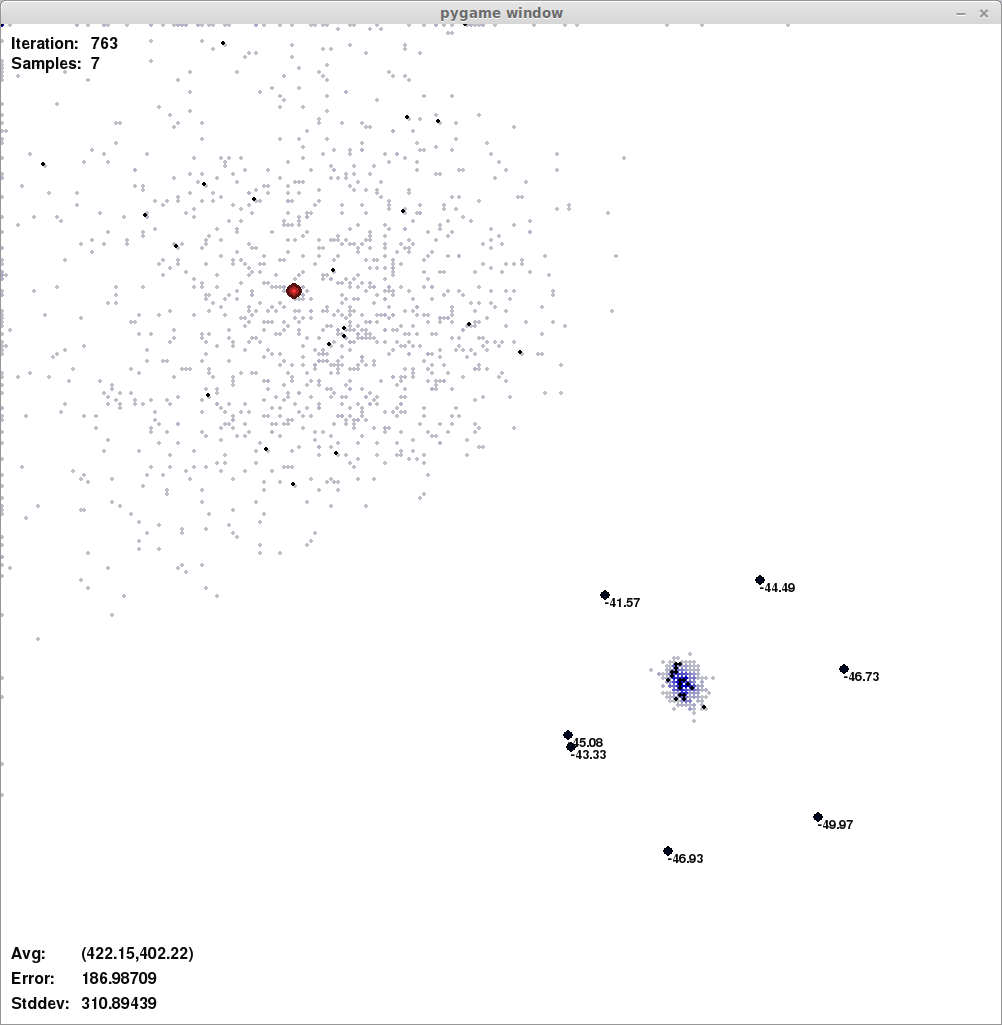
\includegraphics[width=60mm]{ambiguous.png}
  Ambiguous
\end{minipage}%
\begin{minipage}{60mm}
  \centering
  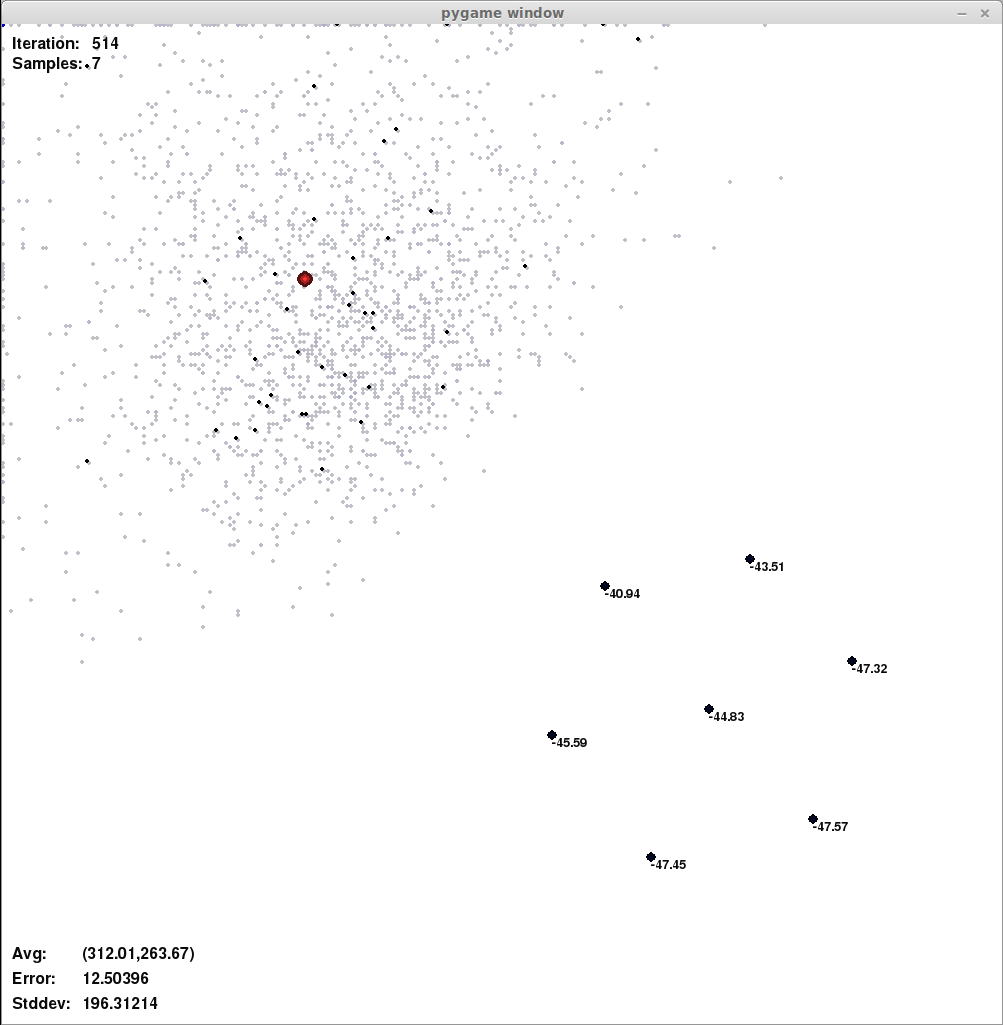
\includegraphics[width=60mm]{nonambiguous.png}
  Non-Ambiguous
\end{minipage}
\caption{Formations with and without ambiguities}
\label{ambiguity}
\end{figure}


Figure \ref{ambiguity} shows two very similar configurations. Both have the same number of sample-points. Each receiver is indicated as a blue circle with a number next to it. The small black or blue points (old predictions are blue) are predictions for the location of the emitter. The emitter is shown as a red circle. In the left image, two samples are placed in the same spot, making it hard to see them both. In the right figure, one of these samples has been moved to cover the central spot in the formation. Moving one of these samples to the middle of the configuration removes an ambiguity that could not otherwise be distinguished based on the sensor-readings. 

Continuing with the same two formations, approaching it by looking at the algorithm, it can be shown that the formation with the ambiguity cannot distinguish between the point in the center of the formation and the actual emitter-location. From the \gls{NLLS} algorithm \gls{PDOA}, Qxy-values are generated as part of making a prediction. These Qxy-values indicate the error, given the measurements of the signal strength and an assumed emitter-location. Simplified, this can be interpreted as: what is the error, compared to the measurements, given that we place the emitter in location (x,y)?


\begin{figure}[H]
\centering
\begin{minipage}{55mm}
  \centering
  \includegraphics[width=58mm]{Ambiguous_-_Emitter_position.png}
  Emitter position
\end{minipage}%
\begin{minipage}{55mm}
  \centering
  \includegraphics[width=58mm]{Ambiguous_-_Wrong_position.png}
  Wrong position
\end{minipage}
\caption{Ambiguous formation}
\label{ambiguousform}
\end{figure}

Figure \ref{ambiguousform} shows the distribution of Qxy-values for two points from the left image in Figure \ref{ambiguity} - the emitter-location and the "wrong position", where it is frequently mispredicting. A prediction will occur at the position that features the lowest error/Qxy-value. From the figure, it is possible to see that whether the Qxy-value for the emitter-location or the center of the formation is the lowest of the two, is likely to be left to chance. This is because the distributions are very similar, and neither has a mean that is significantly higher than the other. 

\begin{figure}[H]
\centering
\begin{minipage}{55mm}
  \centering
  \includegraphics[width=58mm]{Non-ambiguous_-_Emitter_position.png}
  Emitter position
\end{minipage}%
\begin{minipage}{55mm}
  \centering
  \includegraphics[width=58mm]{Non-ambiguous_-_Wrong_position.png}
  Wrong position
\end{minipage}
\caption{Non-ambiguous formation}
\label{nonambiguousform}
\end{figure}


Using the formation shown in the right image of Figure \ref{ambiguity}, removes the ambiguity. The distribution of Qxy-values for the emitter-location has a mean that is significantly lower than that of the center of the formation (Figure \ref{nonambiguousform}). This makes predicting the center of the formation as the emitters-location highly unlikely, if not impossible. 


\begin{figure}[H]
\centering
\begin{minipage}{58mm}
  \centering
  \includegraphics[width=58mm]{Correlation_Ambiguous.png}
  Ambiguous formations
\end{minipage}%
\begin{minipage}{58mm}
  \centering
  \includegraphics[width=58mm]{Correlation_Non-ambiguous.png}
  Non-ambiguous formations
\end{minipage}
\caption{Correlation ambiguity}
\label{ambiguity_correlation}
\end{figure}

Figure \ref{ambiguity_correlation} shows the correlation between the two points for each of the formations in Figure \ref{ambiguity}. Each dot in the figure is one pair of Qxy-values. One from the emitter-location and one from center of the formation. They are coloured green or red, depending on whether it would result in predicting the actual emitter-location or not. The non-ambiguous formation has only green points, however, that does not mean that it will always predict correctly. In Figure \ref{ambiguity}, a large cloud of predictions can be seen in the right image. This cloud is a result of there being many other points on the grid used for \gls{NLLS} that can be chosen (other than the two being compared here). Reducing the size/spread and making the cloud mean-value correct is part of what is investigated in this work.


\subsection{Sensitivity landscape}

Continuing with the same triangle/circle formation that was used for exploring the problem with ambiguities, it is possible to get an indication of the robustness of the predictions, depending on the location of the emitter. In an effort to explore this, a set of plots representing the sensitivity over an area was developed. Figure \ref{slandscape_circle_noise1.5} shows the average error (m) in predictions as a colour gradient. This plot is generated by moving the simulated emitter around the area and measuring the error in positions-predictions generated by the \gls{NLLS} algorithm. 

\begin{figure}[H]
\centering
\includegraphics[width=120mm]{slandscape_15_circle.png}
\caption{Sensitivity landscape with 1.5 dB Gaussian noise}
\label{slandscape_circle_noise1.5}
\end{figure}

In Figure \ref{slandscape_circle_noise1.5}, there are two effects to be noticed:

\begin{itemize}


\item Precision decreases/error increases as the emitter is placed further away from the receivers.
\item A triangle or circle creates an area with anomalies in the center of the circle.

\end{itemize}

The anomalies in the center of the circle is the same effect causing the ambiguities in predictions, as seen earlier. Placing a fourth sample/receiver in the middle of the circle from the previous plot (Figure \ref{slandscape_circle_noise1.5}) removes the anomaly in the center of the circle and gives a smoother overall appearance (Figure \ref{slandscape_twolayer_noise1.5}). This is related to the way \gls{PDOA} calculates emitter-location predictions and is not possible to avoid, unless further information is added to the algorithm. From the perspective of Step 4 (Subsection \ref{P1FC}), this is a problem, as it introduces ambiguities. Based on the sensory readings, it is impossible for the \gls{PDOA} algorithm to distinguish between an emitter in the middle of the formation and a strong emitter far outside the formation.

\newpage

\begin{figure}[H]
\centering
\includegraphics[width=120mm]{slandscape_15_twolayers.png}
\caption{Sensitivity landscape with 1.5 dB Gaussian noise}
\label{slandscape_twolayer_noise1.5}
\end{figure}

Increasing the noise added to the measurements does not change the general traits in any significant way. The only change is a narrowing of the dark blue areas (with good accuracy). In effect, this results in a smaller area in which good prediction precision can be achieved.



\subsection{Optimizing angles}
\label{R_FL_OPT_ANGLES}

So far, only a formation consisting of individual points has been considered. As mentioned previously, the additional computational capacity allows for exploring formations with more samples. Considering a string of sample-points, a set of way-points for a \gls{UAV} is also possible. A simple, but inflexible optimization-scenario is a set of paths moving away a from a single point. As was seen in the plots under Sensitivity landscape, accuracy increases as the emitter moves closer to one of the sample-points. It would therefore not be unreasonable to assume that a path moving towards the emitter gives good prediction accuracy. 

\newpage

Using 3 \glspl{UAV}, sending two \glspl{UAV} in direction of the emitter, while optimizing the angle of the last, allows for the visualization of the results in an easy-to-grasp manner. Figure \ref{optangles_60deg_3uavs} show two visualizations of the same data:

\begin{enumerate}
\item A graph over the angle of the last path, plotted against the fitness (Subsection \ref{MFS3}) of the formation.
\item A visualization showing the outline of the two paths towards the emitter, and the third path indicated as a colour gradient. Blue colour indicates high fitness and good predictions, while white colour indicate poor prediction accuracy. 
\end{enumerate} 


The distance between each sample is assumed to be constant. This is given by a constant sampling-frequency and an assumption of a constant travelling speed for each \gls{UAV}. The distance ($D$) between each sample is then $D = V * I$. $V$ is the velocity of the \gls{UAV}. $I$ is the sample interval. 


\begin{figure}[H]
\centering
\begin{minipage}{65mm}
  \centering
  \includegraphics[width=70mm]{optangles/3uavs5steps60deg_1.png}
  Graph
\end{minipage}%
\begin{minipage}{65mm}
  \centering
  \includegraphics[width=65mm]{optangles/3uavs5steps60deg_2.png}
  Visual representation
\end{minipage}
\caption{Optimizing angles of 3 \glspl{UAV} with a 60 degree spread}
\label{optangles_60deg_3uavs}
\end{figure}

As the spread increases between the two fixed paths (Figure \ref{optangles_100deg_3uavs}), it becomes more beneficial to place the path for the last \gls{UAV} between the two already placed. The result of this placement, is a fan-like formation, spanning less than 180 degrees in the direction of the emitter. 

\begin{figure}[H]
\centering
\begin{minipage}{58mm}
  \centering
  \includegraphics[width=58mm]{optangles/3uavs5steps100deg_1.png}
  Graph
\end{minipage}%
\begin{minipage}{58mm}
  \centering
  \includegraphics[width=58mm]{optangles/3uavs5steps100deg_2.png}
  Visual representation
\end{minipage}
\caption{Optimizing angles of 3 \glspl{UAV} with a 100 degree spread}
\label{optangles_100deg_3uavs}
\end{figure}



\begin{figure}[H]
\centering
\begin{minipage}{58mm}
  \centering
  \includegraphics[width=58mm]{optangles/3uavs5steps80deg_1.png}
  Graph
\end{minipage}%
\begin{minipage}{58mm}
  \centering
  \includegraphics[width=58mm]{optangles/3uavs5steps80deg_2.png}
  Visual representation
\end{minipage}
\caption{Optimizing angles of 3 \glspl{UAV} with an 80 degree spread}
\label{optangles_80deg_3uavs}
\end{figure}

There is a gradual trade-off between placing the last path in the middle, between the two already placed paths or backwards, away from the emitter. The deciding factor is, for the most part, the angle of the spread between the two already placed paths. This can be seen in Figure \ref{optangles_80deg_3uavs}.

In this limited search space, there seems to be two local maxima. One is found using a spread of approximately 50 degrees, and with the last path away from the emitter. The other solution is using a more general fan-formation, with a spread of 100-150 degrees, placing the last path in-between the two already placed. Plotting this entire search space as a two-dimensional plot, with the spread between the two already placed paths on the Y-axis, and the angle of the last path on the X-axis, results in the following plot (Figure \ref{optangles_overview_3uavs}).


\begin{figure}[H]
\centering
\begin{minipage}{70mm}
  \centering
  \includegraphics[width=80mm]{optangles/3uavs5stepsoverview.png}
  Overview
\end{minipage}%
\begin{minipage}{55mm}
  \centering
  \includegraphics[width=55mm]{optangles/3uavs5steps60deg_2.png}
  Visual representation
\end{minipage}
\caption{Overview of optimization of angles for  3 \glspl{UAV}}
\label{optangles_overview_3uavs}
\end{figure}

These plots were generated and smoothed using two techniques; the random seed is reset for each angle being tested, and 500 trials/predictions were run for each angle. Together, these two techniques smooth the graphs and account, to some extent, for the uniform colour transitions, as seen in the plots. 

As can be seen from Figure \ref{optangles_overview_3uavs}, there is two areas showing greater fitness than the rest. This leads to a theory that there is, in general, two ways to proceed if good predictions are required:

\begin{enumerate}
\item Placing two paths facing forward, with the last path backwards, away from the emitter (Scorpion, as in Figure \ref{optangles_60deg_3uavs})
\item Using a more general fan-formation, spreading the \glspl{UAV} evenly in a span of 100-180 degrees, towards the emitter. (Scattershot, as in Figure \ref{optangles_100deg_3uavs})
\end{enumerate}

\begin{figure}[H]
\centering
\begin{minipage}{60mm}
  \centering
  \includegraphics[width=65mm]{optangles/3uavs5steps100deg_2.png}
  Scattershot
\end{minipage}%
\begin{minipage}{60mm}
  \centering
  \includegraphics[width=65mm]{optangles/3uavs5steps60deg_2.png}
  Scorpion
\end{minipage}
\caption{Two good solutions for 3 \glspl{UAV}}
\label{optangles_scat_scorp}
\end{figure}

The formation nicknamed Scattershot features a wide spread (100-180 degrees) in the general direction of the emitter. Comparing the fitness-values of this to that of the Scorpion formation, Scattershot has slightly worse fitness-value (aprox. 2.75 vs 3.25). Scorpion formation has a similar fan-out formation as Scattershot, but in addition, one \gls{UAV} is kept back, forming what resembles a tail. The tail appears to narrow down the spread of the fan-formation to about 60-100 degrees, in the general direction of the emitter. The direction of the tail seem to be fairly robust against minor direction-alterations.

It should be noted that these two formations are not the only options available. There is a multitude of variants in-between these formations. As can be seen in Figure \ref{optangles_overview_3uavs}, there is a gradual change and large areas which provide decent performance, if not optimal. It is not unlikely for a \gls{GA} or \gls{MOEA} to get stuck in these areas. The chance of getting stuck in a local maximum increases when adding the possibility of a favourable selection of random noise (in the fitness-evaluation).


Increasing the degrees of freedom in the optimization is possible, however, this also significantly increases the size of the search space. Exhaustive search becomes hard in such a large search space -  instead, a \gls{GA} is applied. By applying a \gls{GA}, it is no longer possible to guarantee that the optimal solution is found, only that good solutions will be found.

\newpage

\section{Complete path}


\label{Res_CP}

Previous scenarios considered only straight-line paths. In a real-world application, there is no constraint forcing the paths to be straight lines. Allowing for curved paths is a logical extension to find potential even better solutions. The \gls{NLLS} algorithm requires spacial difference in all dimensions to predict accurately, which a single straight line does not offer. Using a \gls{GA} and the encoding described in Subsection \ref{EAGENOMEPATH} - one angle per step of the path for each \gls{UAV} - additional freedom is given to the solutions. The drawback is a large increase in the search space. 

Using a \gls{GA} on this problem is a challenge. The multi-modal fitness landscape, as seen when optimizing an angle, is likely to gain additional local maxima as a result of the increased freedom in solutions. The large search space means that it is not feasible to hope to examine all the possible solutions. Determining the fitness of a formation/set of paths, is a non-deterministic non-linear simulation that requires significant computation to be statistically significant.

\begin{table}[H]
\centering
\caption{Parameters for Complete path optimization}
\begin{minipage}{50mm}
\small
\begin{tabular}{l l}
Population size & Number of UAVs * Number of steps * 20   \\  
& \\
Num. trials & 100  \\
Num. gen. & 100  

\end{tabular}
\end{minipage}
\centering
\begin{minipage}{50mm}
\small
\begin{tabular}{l l}
& \\
& \\
Crossover rate & 0.7 \\ 
Mutation rate & 0.05 

\end{tabular}

\end{minipage}
\label{FIG_CP_PARAMS}
\end{table}

The Complete path optimizations were conducted using the parameters listed in Table \ref{FIG_CP_PARAMS}. Mutation rate was set by general guidelines, between 0.05 (5\%) and 0.10 (10\%). Crossover rate was set to 0.7 (70\%). These parameters could be adapted further to the problem being optimized. In benefit of further exploration of the problem being optimized, this was down-prioritized. Remaining parameters for the simulation can be found in the configuration files in the code archive.

Population size was set, based on the number of genes in the genome. This proved to work well for most optimizations. In some cases, especially with many genes, this may have been insufficient to fully span the solution space. Generally, the solution space grow exponentially as genes are added, the population size as described here, grows linearly. This leads to a situation where the initial population may not fully span the solution space. Solving this would imply increasing the population size significantly. Current optimizations are pushing the limits within the time allotted. Increasing the population size further is outside the scope of this work.

\begin{figure}[H]
\centering
\includegraphics[width=120mm]{uav3steps5.jpg}
\caption{Complete path with 3 \glspl{UAV} and 5 samples each}
\label{completepath_uav3_step5}
\end{figure}



In Figure \ref{completepath_uav3_step5}, the path of three \glspl{UAV}, each with 5 steps/samples, have been optimized. The performance-criteria used was precision in prediction-estimates. Each black dot in the plot is one prediction, using the formation indicated. As can be seen in the figure, two \glspl{UAV} are focused on moving towards the emitter-location. It is not beneficial for them to move in straight lines towards the emitter, as this would yield little information. The result is a path where the two  \glspl{UAV} converge on the emitter, but avoid moving straight towards it to maximize the value of each of their sample-points. The last \gls{UAV} moves away from the emitter; this is consistent with the results from Subsection \ref{R_FL_OPT_ANGLES}.



\begin{figure}[H]
\centering
\begin{minipage}{60mm}
  \centering
\includegraphics[width=65mm]{uav4steps5.jpg}
  5 \glspl{UAV}
\end{minipage}%
\begin{minipage}{60mm}
  \centering
\includegraphics[width=65mm]{uav5steps5.jpg}
  6 \glspl{UAV}
\end{minipage}
\begin{minipage}{60mm}
  \centering
\includegraphics[width=65mm]{uav6steps5.jpg}
  7 \glspl{UAV}
\end{minipage}
\begin{minipage}{60mm}
  \centering
\includegraphics[width=65mm]{uav7steps5.jpg}
  8 \glspl{UAV}
\end{minipage}
\caption{Complete path - 5-8 \glspl{UAV} - 5 steps}
\label{FIG_CP_4_7}
\end{figure}


With five \glspl{UAV}, four \glspl{UAV} have chosen a more-or-less direct approach towards the emitter, apart from the deviation required to not move in a straight line towards the emitter. The four \glspl{UAV} moving towards the emitter are partially intertwined, which was a characteristic common to a number of solutions from the \gls{GA}. The \gls{GA} got stuck in this solution, unable to untangle the paths. For the \gls{GA} to untangle the paths towards the emitter, a sequence of favourable mutations would have to occur, which is an unlikely event. The last \gls{UAV} acts as an anchor, going in the opposite direction of the emitter. By going in the opposite direction of the emitter, this \gls{UAV} is able to exclude any chance that the emitter may, in fact be in the other direction, and for some formations this also removes ambiguities. 

Adding another \gls{UAV} for a total of six \glspl{UAV}, the paths evolved feature a wider spread than for five \glspl{UAV}. This is a fairly uncharacteristic solution; more common would be a narrow spread towards the emitter ($< 180$ deg.). The paths developed show an attraction towards the emitter, but the paths are less predictable than for three or five \glspl{UAV}. The addition of more samples increase the information available. Seen in relation to earlier experiments: that an increase in number of samples would increase the precision of the estimates, it is logical to assume that it may also make the formation less sensitive to the individual placement of the samples.

For both seven and eight \glspl{UAV} (Figure \ref{FIG_CP_4_7}), the situation remains similar to previous results. Most of the \glspl{UAV} will commit to a path towards the emitter-location, while one or two (increasing with the total number of \glspl{UAV}) will remain, or move away from the emitter, eliminating the possibility of the emitter being in that direction and resolving ambiguities. It can be seen that the formations have degraded some - while the general characteristics remain the same, the paths resulting from the optimization are no longer equally smooth. This was seen in a number of similar runs and is accredited the increase in informations available, in addition to the increased size of the search space. 

The results presented here are single runs from the \gls{GA}. There is a significant amount of noise in the results. The main culprit of this is lack of computational resources; even using massive parallel computation (\gls{CUDA}), additional processing would be useful. Each individual in the population is evaluated by doing 100 predictions. According to the formulas for fitness-calculation, these predictions then form a fitness-value, which is used to estimate the performance of the individual. Unfortunately, being able to use 1000 predictions for each evaluation would have been better, but this would have increased the run-time of the optimizations by a factor of 10. Using 100 predictions, there are cases where the individual is able to get a favourable draw of noise. Favourable draw of noise might lead to the solution getting better performance-scores than their real scores. Multiple runs were executed with similar results as these (using different initial seed). Computational restraints also made it impossible to increase the population size further.
\newpage
Another cause of noisy solutions is: indifference. As the number of sample-points increases, the selection pressure to select an optimal location for each sample lessens. This is both a positive trait, in that solutions appear robust against slight variations in placements, but also negative, in that there is no one clear-cut solution to the problem that can be extracted.

Normally, solutions from a \gls{GA} is compared and analysed by conducting numerous experiments and using averaging or similar operations on the results. This would have given the results greater credibility. The results in this optimization is a set of paths for a group of \glspl{UAV}. Comparing the solutions between runs proved difficult. An average solution have little meaning in this context. Attempts were made to plot results from a set of runs in the same figure, but even very similar formations often featured rotation which amplified any differences when viewed in a single figure. It was concluded that it may not be possible to do meaningful statistical review of the solutions generated. This is a shortcoming that proved difficult to surpass, which is part of the reason for exploring heuristics instead of "blueprint"-solutions later in this work (Section \ref{RA_HEUR})

The \gls{GA} uses full generation replacement along with elitism of two individuals, to maintain good solutions. While elitism ensures that known good solutions are kept, it can also be problematic. In this case, the fitness-evaluation is a noisy simulation. The noise in the simulation can greatly affect the performance of the solution, both for better and worse. Solutions are also only evaluated once: old solutions that are kept are not re-evaluated. This opens up for the possibility that a solution could attain a favourable selection of noise, giving it a better fitness-estimate than it should have had. Using the \gls{GA} without elitism and with re-evaluation, resulted in an insurmountable amount of noise in both intermediate solutions during optimizations and final solutions. The conclusion from this was that noise in these optimizations is a problem. Further work might include a more thorough exploration of this issue.

Looking at the results from a qualitative perspective, there are a few general traits characterising most of the solutions:

\begin{enumerate}
\item Move towards the emitter
\item Fan formation
\item Use a 180 degree span.
\end{enumerate}

Moving towards the emitter is beneficial. From the \gls{PL} model it is clear that the \gls{RSS} increases rapidly for samples taken closer to the emitter. This causes noise to become a minor factor, and increases precision in predictions greatly. Just by having a single sample of the \gls{RSS} fairly near the emitter, excellent predictions are possible. This is discovered early on by the \gls{GA}, as it focuses most of the resources to move \glspl{UAV} towards the emitter-location. In itself, this is a useful discovery, however, in an effort to discover a strategy going from having no information of the emitters-location to knowing where the emitter is, there is limited use for this knowledge.



\begin{figure}[H]
\centering
\includegraphics[width=120mm]{uav6steps4.jpg}
\caption{Complete path with 6 \glspl{UAV} and 4 steps}
\label{completepath_uav6_step4}
\end{figure}

Figure \ref{completepath_uav6_step4} shows another variant of the solution. This is from the same set of runs as the previous solutions, but using only 4 steps instead of 5. There is a wider spread of the fan-formation towards the emitter in this solution. Solutions with more steps show a greater tendency of stretching towards the emitter. With more steps, the \glspl{UAV} can get closer to the emitter, and this becomes a driving factor in prediction precision. With less steps, as is the case for Figure \ref{completepath_uav6_step4}, none of the \glspl{UAV} are able to get close to the emitter with the number of steps available. As such, a better solution is to spread out more, and instead try to sample as large an area as possible to increase prediction precision.


\begin{figure}[H]
\centering
\includegraphics[width=120mm]{uav1steps9.jpg}
\caption{Complete path with 1 \gls{UAV} and 9 samples}
\label{completepath_uav1_step9}
\end{figure}


In the case of only one \gls{UAV} and 9 steps (Figure \ref{completepath_uav1_step9}), the \gls{UAV} is able to pinpoint the location of the emitter quite well. There is, however, one caveat with the path that has been evolved here. By moving directly towards the emitter and only using the last step to sidestep, the predictions have low average error and variance, but this is also presumptuous. At the beginning of its path, the \gls{UAV} cannot know in which direction the emitter is, even so, the \gls{GA} has chosen a path heading straight for the emitter. This is an effect caused by the \gls{GA} introducing more information than it should, through the evaluation of the fitness of the path. By allowing the path to optimize against the actual position of the emitter, information that would not be available at the time the path was decided is introduced to the path selection. Because of this, the viability of the strategies/plans developed was put into question. Optimally, the solution to finding the emitter is to go to where the emitter is and measure the \gls{RSS} at that location. This solution, obviously, only works if the location of the emitter is already known. Further exploration was required to develop a robust strategy. 

Knowing the emitter-location is a problem when trying to implement an incremental strategy for path-planning, using these results. Without knowing exactly where the emitter is located, the \gls{UAV} could not possibly know that the path, as seen in Figure \ref{completepath_uav1_step9}, would be optimal, let alone which direction to chose at the start. In order to address these problems, an "Incremental path" approach is suggested. Developing the path incrementally, first for 3 steps, then for the next 3, adds a requirement that the path for $N$ steps is also a part of the path for $N+M$ steps. This makes it impossible for the path, as seen in Figure \ref{completepath_uav1_step9}, to be used, as the first 3 steps would result in high prediction-error.




\newpage

\section{Incremental path}

\label{Res_IP}


Incremental path optimization consists of a fixed prefix and a path to be optimized. The prefix is immutable for the duration of the optimization, and only the appended path is available for the \gls{GA} to change. An implication of this, is that the first steps are optimized as if the last part of the path did not exist. There are multiple interpretation of this:

\begin{enumerate}

\item Getting usable predictions without waiting for more data
\item Avoiding a situation where the \gls{GA} assumes that all the measurements will be included
\item Generating paths that are robust to \gls{UAV} failure
\end{enumerate}

Incremental path puts pressure on the \gls{GA} to select solutions that, not only result in good accuracy of predictions, but also provide useful data during the path traversal. This is a very useful attribute, since getting some general indication of the emitter-location along the way is valuable for an end user.

The prefix is generated in the same way the solutions for the Complete path are generated. In other words, to generate a 3-step prefix for 3 \glspl{UAV}, the Complete path optimization is used. It would be possible to do more increments, i.e having a base prefix of 3 steps and to do multiple increments of 3 steps each. For the results described here, only one increment was applied and optimized.

Fitness is evaluated as if all of the points, both in the prefix and in the appended path, was part of the genome to begin with. This is reasonable, as the samples accumulated through the prefix path will also be available to help the location-predictions. 

As a result of the immutable prefix, the \gls{GA} has limited ability to affect the behaviour of the prediction produced, given the path. This made using an increment with too few steps of limited interest, as the \gls{GA} had limited opportunity to affect the outcome of the predictions. A minimum of 2-step increments were used in these optimizations.




The main parameters used for the Incremental path optimization are listed in Table \ref{TAB_INCR_PARAMS}. These are very similar to those used for Complete path.

\newpage

\begin{table}[H]
\centering
\caption{Parameters for Incremental path optimization}
\begin{minipage}{50mm}
\small
\begin{tabular}{l l}
%\textbf{Receivers} & \textbf{Error (m)} & \textbf{Gain (m)} \\ \hline
Population size & Number of UAVs * Number of steps * 10   \\  
& \\
Num. trials & 100  \\
Num. gen. & 100  
\end{tabular}
\end{minipage}
\centering
\begin{minipage}{50mm}
\small
\begin{tabular}{l l}
%\textbf{Receivers} & \textbf{Error (m)} & \textbf{Gain (m)} \\ \hline
& \\
& \\
Crossover rate & 0.7 \\ 
Mutation rate & 0.1 
\end{tabular}
\end{minipage}
\label{TAB_INCR_PARAMS}
\end{table}


\begin{figure}[H]
\centering
\includegraphics[width=100mm]{incr2steps/3uavs.jpg}
\caption{Incremental path with 3 \glspl{UAV} and 2-step increment}
\label{incrpath_uav3_step2}
\end{figure}


Figure \ref{incrpath_uav3_step2} shows a 2-step increment added to a 2-step prefix, using 3 \glspl{UAV}. Using a small number of initial steps, the \gls{GA} shows a tendency to spread out, more-or-less evenly, in every direction. As more steps are added, through increments or as part of the prefix, these steps are used in one of two ways:

\begin{enumerate}
\item Moving closer to the emitter-location
\item Acting as a counterbalance, moving away from the emitter
\end{enumerate}




\begin{figure}[H]
\centering
\begin{minipage}{60mm}
  \centering
  \includegraphics[width=65mm]{incr2steps/4uavs.jpg}
  4 \glspl{UAV}
\end{minipage}%
\begin{minipage}{60mm}
  \centering
  \includegraphics[width=65mm]{incr2steps/5uavs.jpg}
  5 \glspl{UAV}
\end{minipage}
\begin{minipage}{60mm}
  \centering
  \includegraphics[width=65mm]{incr2steps/7uavs.jpg}
  7 \glspl{UAV}
\end{minipage}
\begin{minipage}{60mm}
  \centering
  \includegraphics[width=65mm]{incr2steps/8uavs.jpg}
  8 \glspl{UAV}
\end{minipage}
\caption{Incremental path - 2-step increment}
\label{FIG_INCR_4_8}
\end{figure}


Figure \ref{FIG_INCR_4_8} shows examples of Incremental path optimizations for 4-8 \glspl{UAV}. These are similar to the results from Complete path (Section \ref{Res_CP}), but they have additional pressure on spreading out early on. This pressure is reduced as more \glspl{UAV} are added. Solutions for 7 and 8 \glspl{UAV} are similar to the results found when using the Complete path optimization.

\newpage

Whenever there is only a small amount of data/samples available, predictions are likely to be highly erratic. Using few steps and/or few \glspl{UAV} will not result in good predictions. There is a connection between the spread of the samples and the accuracy of the predictions. Assuming it is not possible to add more data to the predictions, each sample has to be placed carefully to maximize the utility of that sample. Placing the samples close to, or on top of each other is less beneficial than spreading the samples out over a greater area. In other words, with limited amount of sample-points, a good strategy is to spread them out as wide as possible. Once additional information is added, for instance by adding more steps to each \gls{UAV}, this strategy becomes irrelevant and there are better options to pursue. The important factor with few samples and a comparatively large distance to the emitter, is the spread of the samples and the area covered by the samples.

As the amount of data increases, by increasing the number of steps through an increment, the trend changes. By adding an additional 2 or 3 steps, the steps are no longer spreading out as evenly (as in the prefix path). Instead, an attraction towards the emitter is seen. Samples taken closer to the emitter are of greater help to narrow down the probable locations. This leads to a situation where the \glspl{UAV} appear to converge on the emitter-location. It is still beneficial to have some distance between the samples, as two samples close together add little information to the system.

In a way, the converging phenomenon appears to function much like an attraction force. It is therefore not unreasonable to assume that this may be modelled as an attraction force, using the current best, most likely, location of the emitter as the attraction-point. This is the basis for the Attraction heuristic. There is, however, a few challenges when trying to model this attraction force; in particular, how strong should the force be and how does the distance to the emitter effect the attraction force?

Solutions for different numbers of \glspl{UAV} vary greatly. This may be seen as a result of highly specialized solutions, generated by the \gls{GA}. Comparing the solutions across number of \glspl{UAV} is challenging. In order to relieve this problem, a \gls{MOEA} may be applied, allowing the optimization of formations with different numbers of \glspl{UAV} at the same time. The advantage of this approach is the sharing of genetic material between solutions with different numbers of \glspl{UAV}.


\newpage

\section{Multi-objective path}

\subsection{Motivation}

When a \gls{MOEA} is used to optimize, several objectives are considered at once. Unlike the \gls{GA}, a \gls{MOEA} does not conclude with a single best solution, but a set of good solutions. This is also known as a set of solutions on the pareto front. These solutions will try to describe the best of both worlds, given two criteria to be optimized. They represent solutions to which no better alternatives have been found, unless one is willing to sacrifice performance in the other criteria/objectives. In other words, the result of a \gls{MOEA}-optimization is a set of solutions, which showcase good choices for solving the problem. It is then up to the user to infer which solution is best suited, given the user's preferences.

The \gls{MOEA} separates part of the optimization-process from the decision-making process. By presenting a set of solutions instead of a single solution, an additional choice has to be made in order to fully solve the problem. This is, generally, considered expert knowledge. A person, or user, with expert knowledge about the problem, may use the set of solutions generated to help in a decision-making process. In a way, this can be thought of as the \gls{MOEA} exploring and highlighting the options of interest, while leaving the final decision to be taken, based upon the preferences of the user or expert.

In this research, there were three reasons for using a \gls{MOEA}:

\begin{enumerate}
\item Analysing the trade-off between two objectives/attributes of the solutions
\item Reducing variation in results from the \gls{GA} across runs
\item Introducing a more flexible and realistic genetic encoding
\end{enumerate}

Analysing the trade-off between two objectives is important to know what the consequences of the choices made are. For instance, should an operator that has 20 \glspl{UAV} available commit all 20 to search for one emitter, or use 5 \glspl{UAV} and a bit more time? Should the \glspl{UAV} move fast and cover a lot of ground, or slowly and get data with a higher resolution over a smaller area? This type of reasoning was also used in development of these systems, as it was unclear how fitness-evaluation should combine both variance and average error to a single fitness-estimate for the \gls{GA}. 


The results from the \gls{GA} showed a great deal of variation between runs. A common cause for this is that the \gls{GA} has not been allowed to run for enough generations, leaving the final result in a state of partial convergence. From the results, this does not appear to be the case, as no more progress was made for many generations before the search was terminated. This variation is assumed to be caused by a fitness landscape featuring a few clearly defined preferences, but at the same time being indifferent in a lot of cases. To reduce the variation in the results, the \gls{MOEA} allowed solutions to inherit traits across, what would for the \gls{GA} be multiple runs. This made for a more uniform set of solutions, and aided in comparing and analysing results.

Finally, introducing a more flexible and realistic genetic encoding was possible, as solutions could be described, by the encoding, that would not degrade to a trivial solution. An example of this is the precision and step-length encoding. If step length had been introduced as a parameter to the \gls{GA}, it would likely have chosen to maximize this attribute as to reach the emitter with at least one \gls{UAV}. This can be seen from the Complete path results (Table \ref{TAB_CP_RES_45} in Appendices chapter), as paths that come close to the emitter will result in high prediction accuracy.  Once at least one \gls{UAV} is able to sample the signal very close to the emitter, all other samples become of little value, and the solutions become trivial. By introducing the step-length gene, and at the same time adding the maximum step length as an objective to be minimized, the \gls{MOEA} is forced to make a trade-off between precision and general proximity to the emitter-location. Proximity to the emitter-location is a strong factor in decreasing the error in predictions and increasing accuracy. 



\newpage



\subsection{Variance}

While working with the \gls{GA}, it appeared as if average error in predictions was an insufficient mean of describing performance characteristics. This is best explained by considering two distinct sets of predictions; on a ring with a radius of R and in a single point, a distance R from the emitter. The naïve approach of an average error in prediction-estimate, makes the two different sets of predictions equivalent in terms of the final value describing them. This is because taking only the average error, compared to the actual emitter-position has no way to differentiate between the two. One idea that was attempted was to use not only the average error, but also the variance of the predictions, to better describe the performance characteristics of the formation being evaluated. Figure \ref{MOEA_VAR_SOLUTION} shows a solution from optimizing variance against average error.



\begin{figure}[H]
\centering
\includegraphics[width=105mm]{variancemoea_gen1000.png}
\caption{Variance \acrshort{MOEA} Generation 1000}
\label{MOEA_VAR_SOLUTION}
\end{figure}

\newpage

\begin{table}[H]
\centering
\caption{Parameters for variance optimization}
\begin{minipage}{50mm}
\small
\begin{tabular}{l l}
%\textbf{Receivers} & \textbf{Error (m)} & \textbf{Gain (m)} \\ \hline
Population size & 100   \\  
New individual per gen. & 50  \\
Num. trials & 100  

\end{tabular}
\end{minipage}
\centering
\begin{minipage}{50mm}
\small
\begin{tabular}{l l}
%\textbf{Receivers} & \textbf{Error (m)} & \textbf{Gain (m)} \\ \hline
Crossover rate & 0.7 \\ 
Mutation rate & 0.1  \\ 
Num. gen. & 1000  

\end{tabular}

\end{minipage}

\label{TAB_MOEA_VAR_PARAMS}
\end{table}

The parameters used for optimizing variance against average error is listed in Table \ref{TAB_MOEA_VAR_PARAMS}. The \gls{MOEA} uses a generational mixing replacement, with a maximum number of new evaluation per generation. For this optimization, an additional 50 new individuals were evaluated for each generation.

Early on, it was assumed that it would be possible to find a formation or a set of paths for a group of \glspl{UAV}, that result in predictions featuring any combination of variance and average error. This can be considered as having a formation that delivers low average error in predictions with a large spread, or a small spread with high average error in predictions. The assumption included that it would be very hard for a formation to be good at both at the same time, making specialized solutions, featuring either low average error or low-variance predictions, possible. 

The result from the \gls{MOEA} suggests that the trade-off, if any, is not large enough to be significant, and that a solution, be it a formation or a set of paths for a set of \glspl{UAV}, can have a both a low average error and have low-spread set of prediction. The pareto front, from optimizing variance against average error in predictions, is degraded to a single solution featuring low average error and low variance (good in both objectives). Based on these results, the conclusion must be that variance and average error has little or no trade-off. This is consistent with the results from the \gls{GA}, that show that optimized formations narrow down both variance and average error as resources increase (number of \glspl{UAV} and number of steps).

One of the main reasons for exploring the trade-off between variance and average error, was to evaluate the fitness-function used for the \gls{GA}. At times, the results from the \gls{GA} showed signs of degraded solutions, where the search had managed to find solutions that were not interesting, but had good fitness-values (compared to nearby solutions). Generally, it was found that the \gls{GA} excelled at finding holes in the fitness-function. As previously noted from the project assignment, making good fitness-estimators for this problem is hard; most notably, because normalization of the performance-values of a solution is challenging. The conclusion of this experiment was that it \textit{is} possible to have formations that feature both low average error and variance. Using variance multiplied with average error as part of the fitness-evaluation is not optimal, but is currently the best, most robust solution known.

\newpage


\subsection{\Gls{UAV} count}

\begin{figure}[H]
\centering
\includegraphics[width=70mm]{3_steps/Generation_1000/Pareto_0.png}
\caption{Precision and \gls{UAV} count. 8 \glspl{UAV} and 3 steps.}
\label{moea_count_steps3_uavs8}
\end{figure}


In an effort to compare formations for different number of \glspl{UAV}, a \gls{MOEA} scenario that optimizes on prediction precision and \gls{UAV} count was devised. Comparing end-results from individual \gls{GA}-runs can be challenging, as rotation and random factors make it hard to deduce the underlying structure of the solution. By considering instead, the multi-objective problem of optimizing both precision and \gls{UAV} count at the same time, some of the noise present when comparing separate \gls{GA}-runs are removed, as solutions are recombined across different numbers of \glspl{UAV}. An example of this optimization can be seen in Figure \ref{moea_count_steps3_uavs8}



\begin{table}[H]
\centering
\caption{Parameters for \gls{UAV} count optimization}
\begin{minipage}{50mm}
\small
\begin{tabular}{l l}
%\textbf{Receivers} & \textbf{Error (m)} & \textbf{Gain (m)} \\ \hline
Population size & 200   \\  
New individual per gen. & 100  \\
Num. trials & 100  

\end{tabular}
\end{minipage}
\centering
\begin{minipage}{50mm}
\small
\begin{tabular}{l l}
%\textbf{Receivers} & \textbf{Error (m)} & \textbf{Gain (m)} \\ \hline
Crossover rate & 0.7 \\ 
Mutation rate & 0.1  \\ 
Num. gen. & 1000  

\end{tabular}
\label{TAB_MOEA_UAV_PARAMS}
\end{minipage}
\end{table}

Table \ref{TAB_MOEA_UAV_PARAMS} shows the parameters used for the \gls{UAV} count optimization. These are fairly standardized. Population size could have been increased even further, but given 1000 generations, this was not possible in the given time-frame.

\begin{figure}[H]
\centering
\begin{minipage}{60mm}
  \centering
\includegraphics[width=65mm]{3_steps/Generation_1000/Pareto_0.png}
  8 \glspl{UAV}
\end{minipage}%
\begin{minipage}{60mm}
  \centering
\includegraphics[width=65mm]{3_steps/Generation_1000/Pareto_1.png}
  7 \glspl{UAV}
\end{minipage}
\begin{minipage}{60mm}
  \centering
\includegraphics[width=65mm]{3_steps/Generation_1000/Pareto_2.png}
  6 \glspl{UAV}
\end{minipage}
\begin{minipage}{60mm}
  \centering
\includegraphics[width=65mm]{3_steps/Generation_1000/Pareto_3.png}
  5 \glspl{UAV}
\end{minipage}
\caption{\gls{UAV} count - 3 steps and 5-8 \glspl{UAV}}
\label{moea_count_5_8}
\end{figure}

The solutions seen in Figure \ref{moea_count_5_8} are from the pareto front after 1000 generations of optimizations. As can be seen in the figure, the general shapes found using the single-objective \gls{GA} are present. Generally, most of the \glspl{UAV} are sent in the direction of the emitter. Sometimes, one or two are sent in the opposite direction of the emitter, to counterbalance the focus towards the emitter.  

\begin{figure}[H]
\centering
\begin{minipage}{60mm}
  \centering
\includegraphics[width=65mm]{3_steps/Generation_1000/Pareto_4.png}
  4 \glspl{UAV}
\end{minipage}
\begin{minipage}{60mm}
  \centering
\includegraphics[width=65mm]{3_steps/Generation_1000/Pareto_5.png}
  3 \glspl{UAV}
\end{minipage}
\begin{minipage}{60mm}
  \centering
\includegraphics[width=65mm]{3_steps/Generation_1000/Pareto_6.png}
  2 \glspl{UAV}
\end{minipage}
\begin{minipage}{60mm}
  \centering
\includegraphics[width=65mm]{3_steps/Generation_1000/Pareto_7.png}
  1 \gls{UAV}
\end{minipage}
\caption{\gls{UAV} count - 3 steps and 1-4 \glspl{UAV} }
\label{moea_count_3_14}
\end{figure}

For less than 5 \glspl{UAV} (Figure \ref{moea_count_3_14}), there is less consistency in the solutions. Especially, the solutions for 1 and 2 \glspl{UAV} deviate from the rest. This is caused by the way the algorithm calculates the predictions. The case for 2 \glspl{UAV} is similar to that described in Subsection \ref{results_ambiguities}, and the solution for 1 \gls{UAV} makes a line, resulting in little-to-no depth perspective. 

\newpage

Similarly as with the \gls{GA}, the solutions show that there are a few general traits, but that the \gls{MOEA} is indifferent between small changes to the genome. The results show that it is common for a solution for $N$ \glspl{UAV} to be the same as for $N+1$, with one additional \gls{UAV} disabled. This is as expected, due to the information exchanged between the solutions. In certain cases, where the removal of a \gls{UAV} caused the formation to be degraded, there would be a larger, but still minor jump in the formations developed. This jump in the solutions is natural, as the disabled \gls{UAV} leaves a vacuum to be filled. 

The way the genes are encoded, it is trivial for the \gls{MOEA} to move the path of one \gls{UAV} to cover a hole left by the removal of another. By using a relative encoding, a simple change in the first angle for a given \gls{UAV} will cause the entire remaining path of that \gls{UAV} to be shifted along with it. What is lost by such a change would be specific optimizations, which only benefited the path in a certain direction. For example, a curvature that was highly optimized.

The ability to handle the disabling of a \gls{UAV} is related to the robustness of the formation when faced with \gls{UAV} failure. For the solutions generated, only small changes are required going from, for instance, 7 to 6 \glspl{UAV}. This is promising, as it could imply that the loss of the seventh \gls{UAV} did not cause a major disruption to the strategy developed. At the same time, it could be a result of the information-exchange between the solutions for different numbers of \glspl{UAV}. More investigation is required into this matter to be certain of either case. 

Whenever a \gls{UAV} is disabled, it is usually one of the \glspl{UAV} along the edge of the fan-formation. This might indicate that the \gls{UAV}-paths close to the middle of the formation are more important to the performance of the solution. A possible reason for this could be that these are the \glspl{UAV} that will come closest to the emitter at the end of their path. There is a strong connection between the distance to the emitter-location and the accuracy of the predictions. 

From the analysis of Complete path, two general formations, or categories, were introduced: Scorpion and Scattershot. Also in this experiment, similar tendencies were present, although somewhat weaker than previously. This is consistent with results from the \gls{GA} using a large number of \glspl{UAV}, as described in the result section for Complete path. As more information and more samples are introduced, the pressure to select the location of each sample carefully, decreases. 

As was the case for the results from the Complete path experiment, there is a great focus on moving towards the emitter. The cause is assumed to be the same as for the Complete path optimization. By moving closer to the emitter, the samples gathered come from a higher signal-strength position of the Log-Distance path model, and gives a stronger contribution to removing ambiguities and increasing accuracy of predictions.


\subsection{Step length}

Optimizing the step length, in addition to the paths themselves, proved to introduce further variation in solutions. Some of the solutions are shown below (Figure \ref{MOEA_STEPDEV}), but the variation in the solutions made them hard to work with. This optimization was, therefore, not prioritized, and the work was focused on other optimizations.



\begin{figure}[H]
\centering
\begin{minipage}{60mm}
  \centering
\includegraphics[width=65mm]{stepmoea_5uavs_3steps/Pareto_10.png}
\end{minipage}
\begin{minipage}{60mm}
  \centering
\includegraphics[width=65mm]{stepmoea_5uavs_3steps/Pareto_15.png}
\end{minipage}
\begin{minipage}{60mm}
  \centering
\includegraphics[width=65mm]{stepmoea_5uavs_3steps/Pareto_20.png}
\end{minipage}
\begin{minipage}{60mm}
  \centering
\includegraphics[width=65mm]{stepmoea_5uavs_3steps/Pareto_25.png}
\end{minipage}
\caption{\Gls{MOEA} 5 \glspl{UAV}, 3 steps and total path length 220-370m}
\label{MOEA_STEPDEV}
\end{figure}






\newpage

\section{The value of a sample}
\label{RA_WORTH}



Early in the project assignment, an attempt was made to quantify the value of a sample. How much is a sample worth? How much does precision increase when adding a sample? How does prediction error scale with the number of samples? From the project assignment, the results showed that there is a clear diminishing return after a number of samples have been gathered. For the problem, as described under Step 4, this return becomes small after around 4-6 samples (Figure \ref{predictionerrorreceivercount}).

From the optimization done in this work, the \gls{GA} and \gls{MOEA} indicates that getting close to the emitter is important. 4 \glspl{UAV} and 5 steps are comparable in precision to 8 \glspl{UAV} and 4 steps. In other words, unless time is critically short it would be better and more efficient to use another step and less \glspl{UAV}.

Most importantly, ambiguities should be avoided. It is perfectly possible to introduce situations where the predictions gather in two or more locations that are otherwise indistinguishable. This is a problem, and a situation best avoided. Even modelling the predictions would require advanced methods, such as \gls{FMM}. Ambiguities seem to be less of a problem, given larger amounts of samples. During the testing of the heuristics, ambiguities were not a problem. This is likely because of the amount of data collected. As the heuristic gathers more data, the dynamics of the problem become more stable and anomalies are less frequent.



\begin{figure}[H]
\centering
\includegraphics[width=120mm]{diminishingreturns/3mult.png}
\caption{Diminishing returns, using multiples of 3 samples}
\label{dimret3}
\end{figure}

Figure \ref{dimret3} show the decrease in average error of adding more samples as either steps or an additional \gls{UAV}. The number of samples is the number of \glspl{UAV} multiplied with the number of steps. The red line represents adding samples as additional \gls{UAV}. Starting with one \gls{UAV} with 3 steps, adding an additional \gls{UAV} with 3 steps for each jump. The blue line represents adding samples as additional steps. Starting with 3 \glspl{UAV} with 1 step each, adding an additional step to each \gls{UAV} for each jump.

\begin{figure}[H]
\centering
\includegraphics[width=120mm]{diminishingreturns/4mult.png}
\caption{Diminishing returns, using multiples of 4 samples}
\label{dimret4}
\end{figure}


There is a clear stacking-penalty and diminishing return as the amount of samples increases. The table for Complete path (Table \ref{TAB_CP_RES_45}) shows a weak effect from adding more \glspl{UAV}, while adding more steps will lead to near zero error in predictions, as soon as a sample is located close to the emitter. This effect is also shown in Figure \ref{dimret4}. After 4 to 5 \glspl{UAV} there is very little gain from adding more \glspl{UAV}. However, adding more steps show a gain in precision, for up to and including 40 samples (4 \glspl{UAV} and 10 steps each).
 

Robustness can be achieved by increasing the number of samples. As the amount of data increases, the dynamics of this problems become more stable, and less anomalies are present. With few samples there is a greater pressure to select the location of each sample with care. This has to be done in order to not introduce ambiguities and maximize the gain from the sample. 

\newpage

The value of a sample is, generally, a composite of multiple effects. If the sample is used to remove an ambiguity, the sample can be considered quite valuable. Looking past the possible reduction/removal of ambiguous data, the gain from an additional sample would depend on how much data is already available. Increasing the number of steps per \gls{UAV} is the most effective way of increasing accuracy and precision. Increasing the sample count by adding another \gls{UAV} proved to be less effective. 


\newpage

\section{Heuristics for \Glsentryshort{UAV} behaviour}
\label{RA_HEUR}



\subsection{Heuristics}
\label{RA_HEUR_HEUR}

Each of the heuristics implemented attempts to solve the problem of geolocating an unknown \gls{RF} emitter in a slightly different way. These heuristics are a result of the optimizations done (Complete path and Incremental path), and attempts to approximate different traits from the optimized solutions. Three different heuristics were implemented:

\begin{enumerate}
\item Random walk
\item Whack-A-Mole
\item Attraction 
\end{enumerate}



A random walk heuristic was implemented as a baseline for the other strategies. It is generally assumed that this strategy should be the worst, as it ignores all information available and picks a random move at every step. Increasing the amount of samples available reduces the pressure on selecting good positions for each sample. This may make random walk strategy a viable candidate, given enough data. 

Often, the predictions form a complicated pattern, even given a reasonably simple formation. The predictions may group, or cluster, in multiple areas, or spread out over a larger area. Modelling the predictions is a challenge. \Gls{FMM} can be used to approximate complex distributions by using multiple simpler distributions. When using \gls{FMM}, a number of components/distributions are optimized to fit the input data. Each of these components will then indicate points where the predictions cluster. It is assumed that there can only be one emitter, as such, all but one of the components must indicate false positives. Eliminating all of the false positives should lead to the true emitter-location. Whack-A-Mole strategy will attempt to send one \gls{UAV} to each presumed emitter-location to eliminate each ambiguity.

The results of the optimization would suggest that it is beneficial to move closer to the location of the emitter to reduce the error in the predictions. The Attraction heuristic takes the knowledge, that "closer is better", and applies it using an attraction force to where the set of the \glspl{UAV} believe that the emitter may be located. This location does not have to be the correct location, but it can be. Over time, this strategy should converge on the actual emitter-location as ambiguities are resolved. This heuristic is based on the solutions found by the \gls{GA} (Section \ref{Res_CP}).  There are two parameters to this strategy that have to be decided empirically: strength of the attraction force and initial velocity vectors for each \gls{UAV}. 

For the Attraction and Whack-A-Mole heuristic, attraction forces are used to determine the next action to take. This attraction force directly affects the velocity of the \gls{UAV} at each step simulated. A force coefficient is used to scale the contribution of the force, to the velocity for the next step. This is a value between $0$ and $1$. A value of $1$ would imply that the \gls{UAV} should move directly towards the presumed emitter location. A value of $0$ would make the \gls{UAV} ignore the attraction force, continuing forwards, in the current direction. At any given point in time, the position and velocity of the \gls{UAV} is calculated as following:

\begin{eqnarray}
\boldsymbol{x}_\text{avg} &=& \cfrac{1}{n} \sum_{i=0}^{n} \boldsymbol{x}_\text{pred,i}\nonumber \\
\boldsymbol{b} &=& \boldsymbol{x}_\text{avg} - \boldsymbol{x}_\text{uav} \nonumber \\
\boldsymbol{v}_\text{uav} &=& (1-f) * \cfrac{\boldsymbol{v}_\text{prev}}{||\boldsymbol{v}_\text{prev}||} + f * \cfrac{\boldsymbol{b}}{||\boldsymbol{b}||} \nonumber \\
\boldsymbol{x}_\text{uav} &=&  \boldsymbol{x}_\text{uav} + 50.0 * \cfrac{\boldsymbol{v}_\text{uav}}{||\boldsymbol{v}_\text{uav}||} \nonumber
\end{eqnarray}

$f$ is the force coefficient. $\boldsymbol{b}$ is a vector in the direction of the presumed emitter-location.  $\boldsymbol{v}_\text{uav}$ is the current, unormalized velocity vector. $\boldsymbol{v}_\text{prev}$ is the velocity vector from the previous step. The velocity is normalized at each step to give a constant step length of 50m. This is the same step length as was used in the optimizations. For the Whack-A-Mole heuristic $\boldsymbol{x}_\text{avg}$ is replaced with the center-point of a component from the \gls{FMM} model.


\subsection{Characteristics}

Using a random walk heuristic is a poor choice, as it ignores all information available to assist in the search. In choosing a random direction at each step, it rarely moves far away from the initial point, leading to poor coverage of the search area and low performance. Most often, this heuristic would \textit{not} be able to reach the termination threshold. It was therefore excluded from the performance comparison 

Attraction heuristic is predictable and works well. Attraction heuristic calculates a center of gravity for all the predictions available, and uses this as an attraction-point for the \glspl{UAV}. This is a promising and fairly robust strategy. It works well, even with highly erratic initial predictions (as a result of few samples), but quickly converges on the emitter as more data is added. 

Whack-A-Mole tries to eliminate ambiguities as soon as possible. For a set of predictions, multiple points of interest can be found using \gls{FMM}. Each component is then mapped as the attraction-point of one \gls{UAV}. This strategy is similar to the Attraction heuristic, however, as there are multiple attraction-points, it is more unpredictable. The results is often that one or two \glspl{UAV} choose a highly erratic path, compared to the rest. This is caused by insufficient amount of predictions to form a robust model using \gls{FMM}, and a high chance of ambiguities with few samples. See Figure \ref{FIG_HEUR_EXAMPLE} for examples of behaviour.

\begin{figure}[H]
\centering
\begin{minipage}{60mm}
  \centering
  \includegraphics[width=60mm]{./heuristicexamples/attraction.png}
  Attraction
\end{minipage}%
\begin{minipage}{60mm}
  \centering
  \includegraphics[width=60mm]{./heuristicexamples/whackamole.png}
  Whack-A-Mole
\end{minipage}
\caption{Example of heuristics behaviour}
\label{FIG_HEUR_EXAMPLE}
\end{figure}



\subsection{Performance comparison}

A comparison of the performance of the three heuristics was conducted. This comparison has a termination threshold - a minimum required precision in prediction. Several values of the threshold were tested, but only minor differences were experienced, unless very large threshold-values were selected. Using a threshold of 10m error, each of the strategies were simulated 100 times to get a consistent indication of their performance. This was repeated for 3, 4 and 5 \glspl{UAV}. The number of steps indicated in the tables are per \gls{UAV}. To get the total sample count, this number has to be multiplied with the number of \glspl{UAV}. For instance, 10 steps on average and 3 \glspl{UAV} is actually 30 samples in total. There is a distance of 480m between the initial position for the \glspl{UAV} and the emitter. With the step length of 50m, 10 steps are required to reach the emitter.


\begin{table}[H]
\centering
\caption{Strategy performance. Threshold error 10 m. 3 \glspl{UAV}}
\begin{tabular}{c|l|l|l}
\textbf{Strategy} & \textbf{Avg. steps}  & \textbf{Var. steps} & \textbf{Median steps}\\ \hline
Attraction & 11.08 &  0.61  &  11 \\ 
Whack-A-Mole  & 12.24 &  1.34  &  12\\ 

\end{tabular}
%\label{predictionerrorreceivercounttable}
\end{table}


\begin{table}[H]
\centering
\caption{Strategy performance. Threshold error 10 m. 4 \glspl{UAV}}
\begin{tabular}{c|l|l|l}
\textbf{Strategy} & \textbf{Avg. steps}  & \textbf{Var. steps} & \textbf{Median steps}\\ \hline
Attraction & 10.67 &  0.69  &  11 \\ 
Whack-A-Mole & 11.26 & 1.00 &  11 \\ 

\end{tabular}
%\label{predictionerrorreceivercounttable}
\end{table}


\begin{table}[H]
\centering
\caption{Strategy performance. Threshold error 10 m. 5 \glspl{UAV}}
\begin{tabular}{c|l|l|l}
\textbf{Strategy} & \textbf{Avg. steps}  & \textbf{Var. steps} & \textbf{Median steps}\\ \hline
Attraction & 10.27 &  0.77  &  10 \\ 
Whack-A-Mole & 10.37 & 0.73 &  11 \\ 

\end{tabular}
%\label{predictionerrorreceivercounttable}
\end{table}

Random walk heuristic performs worst of the three heuristics. This is as expected, as it ignores the information available. The Random walk heuristic is not included in the comparison, as it frequently failed to attain the required precision in order to terminate the test and had to be terminated manually. 

The second best is Whack-A-Mole. This heuristic often wasted samples and steps going in the wrong direction (relative to the emitter). This is caused by two factors: Whack-A-Mole tries to eliminate ambiguities, and since there can only be one emitter, most of this effort is wasted once the emitter-location is known. The second factor is an unreliable model from the \gls{FMM}; due to insufficient amount of predictions, the model of the predictions is erratic. 

Attraction strategy performs best out of the three strategies. The difference in performance between Whack-A-Mole and Attraction heuristic is minor, especially as the number of \glspl{UAV} increase. The Attraction heuristic may be preferred, since it is much simpler than the Whack-A-Mole heuristic and have equal or better performance, at least in the given test scenario.



\newpage

\section{Heuristic optimization}

\subsection{Premise of optimizations}

Attraction and Whack-A-Mole was found to both be promising strategies for \gls{UAV} behaviour (Section \ref{RA_HEUR}). Compared to Whack-A-Mole, Attraction offers more predictable behaviour, given an attraction force and a set of initial velocities. The parameters of the Attraction force heuristic were previously not optimized in any way. Optimizing these parameters might lead to further improvement to the heuristic's ability to geolocate unknown \gls{RF}-emitters.

Whack-A-Mole strategy uses an \gls{FMM} to make a model of the predictions. In order to generate this model accurately and robustly, many predictions are required. The heuristics operate by taking in a set of predictions and determining the next step for each \gls{UAV}. If the Whack-A-Mole heuristic was to be applied to a real-world scenario, each \gls{UAV} would have to take a large amount of samples for each step ($>> 100$) to make the \gls{FMM}-generated model robust. This is a disadvantage using this heuristic and made the Attraction heuristic the preferred choice for further investigation.

Optimizing was attempted using a real-coded \gls{GA}. The parameters being optimized was a force coefficient, giving the percentage contribution from the attraction force (compared to the current heading), and the initial velocities. Number of steps taken, before the threshold was reached, was used as a performance metric. This proved insufficient for two reasons: first, the integer number of steps did not provide the \gls{GA} with enough information to distinguish good solutions from bad. Second, the \gls{GA} consistently optimized the initial velocities in the same presumptuous way, as the angles from previous optimizations. In short, the \gls{GA} optimized to direct the initial velocities towards the actual emitter-location.

Making a better optimization is possible and was done by using the fitness-value, instead of the number of steps. The fitness-value was calculated based on the positions chosen by the heuristic. In order to not allow the heuristic to get too close to the emitter, a maximum number of samples were specified, to leave the closest sample at an appropriate distance from the emitter (usually around 100m). 


Like for the Complete path optimization, slight rotation in final solutions from the \gls{GA} made it hard to compare solutions. To simplify the optimization, the initial velocities were removed from the optimization, and an even spread was used instead. In the project assignment, during the optimizations for Step 2, a circle or an equidistant triangle lattice was found to be good solutions. Using an even spread with 3 \glspl{UAV}, gives a 120 degree angle between each velocity vector. A 90 degree angle was used for 4 \glspl{UAV} and 72 degree angle for 5 \glspl{UAV}. If not for the effect of the attraction force, the \glspl{UAV} would fly in in straight paths, evenly spaced out, radiating from the initial location. It might still be possible, given an evenly spread-out formation, to gain a performance advantage if the emitter is in a certain direction relative to the formation. Testing the formation in multiple orientations solves this problem.

Having removed the initial velocities from the optimization and replaced them with a fixed spread and a rotation parameter, only two optimization parameters remained: attraction force coefficient and rotation offset. This optimization can be done exhaustively, given a suitable step for both parameters. The result of this is a table with rotation offset on one axis, and force coefficient on the other. These tables become quite large, and as such, only one example of such a table is included here.


\subsection{Optimization results}

\begin{table}[H]
\centering
\caption{Testing of coefficients. 500m distance. 1 dB noise. 3 \glspl{UAV}}
\small
\begin{tabular}{l l l l l l l}
F. coeff.&Angle offset\\
&\textbf{0 deg}&\textbf{20 deg }&\textbf{40 deg}&\textbf{60 deg}&\textbf{80 deg}&\textbf{100 deg}\\ \hline
\textbf{0.00}&1.77&2.10&3.02&3.10&3.14&2.12\\
\textbf{0.05}&2.05&2.44&3.38&3.74&3.37&2.49\\
\textbf{0.10}&2.78&3.15&4.26&4.72&3.86&3.25\\
\textbf{0.15}&4.40&4.76&5.97&6.15&4.67&4.90\\
\textbf{0.20}&7.81&7.81&8.43&7.97&5.89&8.07\\
\textbf{0.25}&11.83&11.58&10.92&9.77&7.60&11.61\\
\textbf{0.30}&14.50&13.95&12.35&11.02&9.46&13.96\\ \hline
\textbf{0.35}&14.79&14.51&12.51&11.55&10.79&14.29\\\hline
\textbf{0.40}&13.52&13.57&11.82&11.53&11.60&13.00\\
\textbf{0.45}&11.77&12.09&10.89&10.89&11.31&10.91\\
\textbf{0.50}&9.84&10.00&9.24&9.09&9.19&6.76\\
\textbf{0.55}&7.01&6.29&5.09&5.84&5.95&4.42\\
\textbf{0.60}&5.16&4.47&3.37&3.57&3.56&3.27\\
\textbf{0.65}&3.91&3.41&2.60&2.48&2.36&2.49\\
\textbf{0.70}&3.04&2.70&2.11&1.92&1.74&2.01\\
\textbf{0.75}&2.42&2.21&1.83&1.60&1.41&1.65\\
\textbf{0.80}&1.97&1.88&1.62&1.39&1.21&1.42\\
\textbf{0.85}&1.68&1.64&1.47&1.25&1.09&1.24\\
\textbf{0.90}&1.49&1.48&1.36&1.15&1.02&1.10\\
\textbf{0.95}&1.36&1.36&1.28&1.08&0.95&1.00\\

\end{tabular}
\label{TAB_HEUR_OPT_SINGLE}
\end{table}

From Table \ref{TAB_HEUR_OPT_SINGLE} it can be seen that using an attraction force coefficient of $0.35$ outperforms all other coefficients, assuming 500m start distance from the emitter and 1 dB noise. Similar tables were generated for all combinations of 300m, 500m and 700m and 1dB, 2dB and 3dB noise. 


\begin{figure}[H]
\centering
\begin{minipage}{55mm}
  \centering
  \includegraphics[width=55mm]{./heuristicexamples/attraction_optimized.png}
  Attraction
\end{minipage}%
\begin{minipage}{80mm}
  \centering
  \includegraphics[width=80mm]{./heuristicexamples/uav4steps5.jpg}
  Old \gls{GA} result
\end{minipage}
\caption{Comparison Attraction heuristic and an older \gls{GA} result}
\label{FIG_ATTRACTION_OPTIMIZED}
\end{figure}




Left part of Figure \ref{FIG_ATTRACTION_OPTIMIZED} shows an example run of the Attraction heuristic using a force coefficient of $0.35$. Right part of Figure \ref{FIG_ATTRACTION_OPTIMIZED} shows a result from a \gls{GA} optimization. This particular result was excluded from Complete path results, as it was from an older batch of results and uses a different mutation operator. The rest of the solutions belonging to the same set of runs, were not equally smooth (this is why the solution for 4 \glspl{UAV} is shown). 

The formation generated by the heuristic now resembles the results from the Complete path optimization (Figure \ref{completepath_uav3_step5} in Section \ref{Res_CP}). Because of the way the Attraction heuristic is implemented, the paths generated by the heuristic will inevitably be smooth. The solutions generated by the \gls{GA} has no similar restriction or limit.


As the noise increases there is no longer a single force coefficient that is consistently better than all others, this is related to the random sampling taken and the increased error in predictions. In cases where multiple coefficients were shown to give similar performance, ties were resolves by taking the average over all the angle offsets. The coefficient with the greatest average was then chosen as the best. At 3 dB noise, the best coefficient shows great variation. Table \ref{TAB_HEUR_OPT_SUM} shows that at 3 dB, the force coefficient no longer reflects the initial distance from the emitter. Further experiments were done using limited noise (1 dB).


\begin{table}[H]
\centering
\caption{Optimized coefficients for 3 \glspl{UAV}}
\small
\begin{tabular}{l l l l}
Distance& Noise & & \\
 & \textbf{1dB} & \textbf{2dB} & \textbf{3dB}\\ \hline
\textbf{300m} & 0.45 & 0.40 & 0.15\\
\textbf{500m} & 0.35 & 0.35 & 0.30\\
\textbf{700m} & 0.25 & 0.25 & 0.25 \\

\end{tabular}
\label{TAB_HEUR_OPT_SUM}
\end{table}



From the results, it appears that the distance to the emitter is the deciding factor of the force coefficient. Noise has a limited effect. The effect of noise is hard to examine as the increased noise makes the performance of the heuristic degrade as well. From visual inspection/testing of the coefficients, it appears that the best choice is a coefficient that makes the \glspl{UAV} converge on the emitter, as seen in Figure \ref{FIG_ATTRACTION_OPTIMIZED}. If the starting position is close to the emitter, the coefficient has to be higher (stronger force). Otherwise, the \glspl{UAV} will just fly by the emitter, unable to stop.




\begin{table}[H]
\centering
\caption{Optimized coefficients for 3-5 \glspl{UAV}. 1dB noise }
\small
\begin{tabular}{l l l l}
Distance & \textbf{3 \glspl{UAV}} & \textbf{4 \glspl{UAV}} & \textbf{5 \glspl{UAV}}\\ \hline
\textbf{300m} & 0.45 & 0.40 & 0.35\\
\textbf{500m} & 0.35 & 0.30 & 0.30\\
\textbf{700m} & 0.25 & 0.25 & 0.20 \\

\end{tabular}
\label{TAB_HEUR_OPT_UAV}
\end{table}

Further optimizations were done for 3-5 \glspl{UAV}. Excluding noise as a contribution to be examined, the results can be seen in Table \ref{TAB_HEUR_OPT_UAV}. Increasing the number of \glspl{UAV} appears to lessen the force coefficient. The result of this is that the \glspl{UAV} will be less attracted to the estimated emitter-position, and potentially take longer to converge on the emitter. As the number of \glspl{UAV} increases, it makes sense to spread these out in a wider fan, covering a greater area. Distance still remains a major factor in determining the force coefficient. 

Selecting the strength of the attraction force appropriately, it is possible to generate a behaviour that results in the \glspl{UAV} orbiting the emitter once they have gotten close enough. This leads directly to Step 4 of the search, where a circle was found to be a good solution in order to achieve robust and accurate predictions.





\newpage

\section{A strategy}

\subsection{Step 2 - Rough predictions}

Originally, it was assumed that even at a distance, a rough idea of the location of the emitter would be possible to attain. Later experiments showed that the predictions made while standing in any formation, far away from the emitter, are very rough. They will give the general direction of the emitter, but little to no positional accuracy. 

It is also possible to induce ambiguities by choosing a poor formation. One example of a poor formation, capable of inducing ambiguities, is a circle. Given a reasonable distance from the emitter and a circle formation, the receivers will be unable to distinguish an emitter in the center of the circle from an emitter far outside the circle. This is described in Subsection \ref{results_ambiguities}. The same effect can also be seen using less samples in a triangle or a square formation.

The ambiguities can be resolved in a number of ways. Assuming a perfect circle, the simplest method of resolving the ambiguities is to place another receiver, or sample, in the middle of the circle. By placing a measurement in the middle of the circle, it is possible to deduce the shape of the \gls{RSS} intensity field. The sample will, in the case of the emitter being in the middle of the circle, show a peak in measured \gls{RSS}. If a peak is found, it indicates that the emitter is in the middle of the circle. In the case of the emitter not being in the center of the circle, no peak is found.

In general, it is suggested that a good formation for Step 2, is to use an equidistant triangle-lattice. Many formations may fulfil the requirements of not introducing ambiguities. To not introduce ambiguities, they must, in some way have two layers of measurements. Increasing the distance between the receivers in an equidistant triangle-lattice, increases the precision of the predictions. Eventually, increasing the distance too much, the spaces in-between receiver-locations may introduce ambiguities as they grow large.

Finally, it is possible to use other external information, such as: approach direction, topology or geographic information, to assist these initial predictions. It is assumed that during Step 2, Step 1 will have been completed. Step 1 includes a convergence of multiple \glspl{UAV} from different locations. Their respective approach-vectors may be used to exclude some areas due to the data gathered while approaching.

\newpage

\subsection{Step 3 - Relocate}

The relocation phase was investigated in this thesis, going from Step 2 to Step 4, converging on the emitter. It is possible to use this time to gather data, maximizing the utility of the resources spent. This is a very complicated problem with a large search space. In addition, the noise in the predictions and solution make patterns hard to discern.

A perfect solution to this step would be the optimal heuristics defining the actions of each \gls{UAV}. Multiple \gls{GA} and \gls{MOEA} optimization-scenarios were implemented and tested. This lead to further questions and questioning of the scenarios themselves. The solutions show tendencies to stretch out the different types of paths implemented, but at the same time, there is a significant amount of noise clouding the solutions. 

The set of solutions from the optimizations often converge on the emitter in one way or another. This indicates that getting to a higher signal-level is beneficial. In other words, moving closer to the emitter is a sound way of decreasing the error in predictions. Two heuristics spawned from this knowledge: Attraction and Whack-A-Mole.

Attraction heuristic assumes that closer to the emitter is better. This is applied to the heuristic as an attraction force, pulling the \glspl{UAV} towards the assumed emitter-location. As this is a continuous search, the \glspl{UAV} cannot know where the emitter is - they only have rough, error-prone predictions to guide them. These are used as a guide for the direction the \glspl{UAV} should explore. The result is a system where the \glspl{UAV} will be drawn towards the center of the predictions. When additional information is added, the center may shift, and the error lessens. Eventually, the \glspl{UAV} will have gathered enough data to exclude any ambiguities, and were often found to be orbiting the emitter (a result of the way the attraction force is implemented).

Whack-A-Mole heuristic takes a different approach, by trying to resolve ambiguities as early as possible. By using \gls{FMM}, it is possible to generate multiple centers of gravity, as used by the Attraction heuristic. Under the assumptions of the simulations, there can only be one emitter - all but one of these clustering of predictions must be ambiguities. By travelling towards each one of the clusters, the \glspl{UAV} will resolve the ambiguities until only one predicted location remains.

Both of these heuristics show promise and offer similar performance, given an error threshold. The Whack-A-Mole heuristic appears to act more randomly and moves less predictably. This is a result of the limited amount of data available when each choice is made. Without a lot of data to generate an \gls{FMM}, the model is highly unstable. Attraction heuristic can be considered a simplified version of the Whack-A-Mole heuristic, as it only has one attraction-point, leading to more consistent behaviour (potentially using less resources).
 
Given a suitable initial velocity for each of the \glspl{UAV}, both heuristics will form fan-like formations approaching the emitter. Performance between the two heuristics are comparable, but a simple Attraction heuristic may be preferred in this setting, considering robustness and predictability. 

Finally, the parameters of the Attraction heuristic were optimized, leading to behaviour similar to that found in solutions during Complete path optimization (Section \ref{Res_CP}). Initial distance from the emitter and \gls{UAV} count was found to both be important factors in determining the strength of the attraction force.




\subsection{Step 4 - Maximize accuracy}

A circle around the emitter is a very good option to maximize accuracy of predictions. As discussed under Step 2, a circle may introduce ambiguities to the predictions. These ambiguities make it hard, if not impossible, to distinguish an emitter in the center of the circle, as opposed to an emitter far away from the formation. This is a problem that should be avoided whenever possible.

One way to resolve this ambiguity is to use an imperfect circle, with one sample-point located outside the circle. Another option is to use an equidistant triangle-lattice, with a sample in center of the hexagon. This type of ambiguity can, in general, be resolved by introducing a two-or-more layered formation. Having two layers in the formation allows for the detection of a peak in the middle of the formation. 

There is a strong correlation between distance to the emitter and prediction accuracy. To maximize prediction accuracy, placing at least one receiver close to the emitter is a good strategy. This can be explained by considering the \gls{PL} model. Close to the emitter, the receiver will measure high \gls{RSS}. As a result, the noise will be less significant and predictions become very accurate.



\newpage

\section{Threats to solution validity}


\gls{NLLS} requires a grid to be specified. This grid effectively defines the possible solutions that the geolocation algorithm may return as a prediction (Section \ref{PDOANLLS}). The grid adds information to the system, since the emitter cannot be outside the grid. For some scenerios, this assumption may hold, but in general, the specification of the grid/search area may greatly affect the performance of the algorithm, both positively and negatively.

Another concern is the ability to test each solution sufficiently. For most of these simulations, 100 trials were run when testing each solutions. If time allowed, 1000 trials should have been used to test each solution, but this would have increased the run time by a factor of 10. As it is currently, noise may give some solutions favourable evaluations. This is unfortunate as, optimally, only the characteristics of the solution itself should be able to affect its performance evaluation.

Evaluating fitness for this problem is complicated. The majority of this work uses a fitness combined of two metrics: spread of predictions (variance) and average error. These two factors are multiplied, as part of the fitness-value. Optimizations revolve around minimizing these two values. It is possible to make solutions that have a low spread (variance) and a high average error. These solutions will have a fairly high fitness-value, as the product of variance and average error is small (relatively). However, a solution with these attributes is most often not of interest, but may be selected by the optimization, due to the high fitness value. The result is the \gls{GA} or \gls{MOEA} converging to a suboptimal solution. Solutions like these, are easily found by manual review in retrospect, but the lack of a more robust fitness-estimation is concerning.


As this implementation also contains a simulation part, with its own non-deterministic components and noise, the chances of an error in implementation is high. Simulating a real environment includes making assumptions about how the real world behaves. These assumption are often simplifications, which may lead to problems, should the simplification not accurately reflect the real world. The model for \gls{RF} propagation I have employed for these simulations ignores many important real-world problems for \gls{RF} propagation such as:

\begin{itemize}
\item Reflections
\item Interference
\item Signal dampening
\end{itemize}

\newpage

\gls{RF} propagation problems may not seem that important, as devices using \gls{RF} emitters are commonplace for most people and work very well. For the purpose of geolocating \gls{RF} emitters, however, these effects cannot be discounted as easily. An unknown and uncooperative emitter alone is not something most consumer-grade \gls{RF} communication systems have to deal with. Using methods based on \gls{RSS}, the dampening of the signal becomes a matter of importance. The dampening is affected by, for instance weather conditions, topography or simply distance above ground. Distance above ground can to a certain degree be account for, but as mentioned in Section \ref{RFPM} there are significant differences between \gls{RF} propagation in the air compared to on the ground.

In a real-world application, emitters are not forced to stand still. A moving emitter would further complicate the setting, as the samples gathered may not reflect the current location of the emitter. This could be handled using a rolling time-window, where samples are only valid/usable for a short time after collection. Alternatively, by not sampling multiple times per \gls{UAV}, time, effectively stands still, making the emitter non-moving. The complications of a moving emitter was not taken into account for the optimizations done in this work. 

Furthermore, in a real-world scenario, there will likely be more than a single emitter. Distinguishing multiple emitters in the same part of the frequency spectrum is a challenge that has not be considered in this work. Further work is required in the area of separating and classifying multiple emitters in a noisy \gls{RF} environment.

Applying a theoretical study, such as this, to the real world is a challenge. Even if the implementation is sound and the results therefore are valid, there may be factors or problems that have not been taken into account. In other words, even a theoretically sound implementation may encounter problems when put into practice.

There is, as always, many problems that may lead to invalid results. In using  \glspl{GA} and \glspl{MOEA}, a host of issues that are not present with deterministic algorithms presents themselves. Algorithms that do not behave predictably to the programmer are notoriously difficult to debug, and prone to contain errors either in logic or in function. Finding these errors is not impossible, but can be very hard. I have tested and verified this implementation, yet I cannot exclude the possibility of remaining errors. 






\chapter{Conclusion and future work}

This chapter is a conclusion to the work conducted. Suggestions for future work made here are based on the problems, experiences and ideas that appeared while working with these problems.


\newpage





\section{Conclusion}

%Hard problem

Geolocation of an unknown, uncooperative \gls{RF} emitter using a \gls{RSS} method \gls{PDOA} \gls{NLLS} in a noisy environment, employing multiple distributed autonomous \glspl{UAV}, while minimizing resource-consumption in a time considerate optimization is a challenging problem. A large solution and search space, with a non-deterministic (noisy) fitness-evaluation with multiple maxima, make solving this problem a non-trivial task. Even so, the work has been a valuable experience in using multiple methods of optimization on real-world problems. In some situations, it was possible to reduce the effect of noise by carefully manipulating the random-number generator to only generate randomness where it was required, to provide accurate and realistic results. This technique was used, for instance, in developing the fitness-plots showing an overview of the fitness-landscape for different situations. By using the same random noise in-between sets of data that should be compared for performance, the noise in the final figures were greatly diminished. This has to be done with great care, as to not introduce random samplings that may favour some solutions over others and invalidate results.

%Divide and conquer

Often, this work turned out to be an exercise in examining and breaking down the problem into smaller, individual pieces and examining each piece with some degree of independence from the overall problem. Doing so while not disrupting the problem itself, and figuring out reasonable subproblems to work on, was one of the greatest challenges in this work. When it was possible to divide the problem, this often lead to breakthroughs, where previously unassailable problems became manageable and tangible. An example of this is, for instance, plots optimizing angles between path for \glspl{UAV}. These provide a much needed, clear-cut solution to a smaller subproblem. However, these extracted subproblems and associated solutions would not have been possible without first exploring the problem at a higher level to determine which parts of the problem could be extracted. As such, the progression of this work has had a major influence on the end result. 

%Proximity to the emitter

Proximity to the emitter is a clear driving-factor for most of the results from the \gls{GA} and \gls{MOEA}. There is a strong correlation between distance to the emitter and prediction accuracy. From "The value of a sample" (Section \ref{RA_WORTH}) it can be seen that adding more \glspl{UAV} is not a fool-proof solution to gain perfect prediction accuracy. As such, anyone seeking to use a system based on the concepts described in this work should be aware that proximity to the emitter is likely to be the limiting factor.

%Ambiguities

Ambiguities proved to be fairly common, given few resources (sample-points). Such ambiguities result in two or more locations, which are indistinguishable based on the emitter-location predictions given. This is a problem for a real-world system based on \gls{PDOA}. To resolve this, a formation/set of locations to sample, has to be chosen with care. An equidistant triangle lattice, is a simple structure that will, in far most cases, not introduce ambiguities in predictions. Multiple formations will fulfil the task without introducing ambiguities. The main requirement for this is to introduce a multiple-layered formation that can detect the actual shape of the \gls{RSS}-field over the area.

%Two good formation types

In the analysis, two good ways of organizing a group of \glspl{UAV} was suggested; these were nicknamed Scattershot and Scorpion. Scattershot would spread all the available \glspl{UAV} out in a cone in the general direction of the emitter. Scorpion would retain a couple of \glspl{UAV}, sending these backwards, away from the emitter. As the total number of \glspl{UAV} increased, so would the number of \glspl{UAV} being sent away from the emitter. These are, by no means, exhaustive solutions, but they are good general guidelines for \gls{UAV}-behaviour in a \gls{RF}-geolocation system. 

%Heuristics 

Based on the optimizations of angles and paths for \glspl{UAV}, two heuristics were developed: Attraction and Whack-A-Mole. The Attraction heuristic approaches the presumed emitter-location at all times. The Whack-A-Mole heuristic uses \gls{FMM} for clustering of predictions, allowing the heuristic to try to eliminate ambiguities in the prediction. Attraction was chosen as the preferred heuristic for greater predictability in behaviour and for being more robust when faced with erratic predictions. The parameters of the Attraction heuristic was also optimized for a particular scenario, resulting in similar behaviour as seen in the results from the Complete path optimization (Section \ref{Res_CP}).


%A strategy

The work conducted here describes in total: a strategy from emitter-detection to emitter-location prediction. Including the work of Jørgen Nordmoen, in using a swarm of \glspl{UAV} to locate an emitter in a large area, this covers the entire progression from "no information" to having an accurate prediction on the emitter-location. I believe, that with technology available today, it should be possible to implement a functional demonstration-platform, proving these concepts.

%Fully distributed system

There is still work remaining in making this a fully distributed system. As it stands today, going from knowing that there is an emitter to knowing where it is, requires cooperation between the different \glspl{UAV}. Cooperation implies communication, which may or may not be viable, depending on the environment and context. More exploration is required to find out how much of this system could be distributed completely, to avoid having to rely on a single point of failure.

\newpage
\section{Future work}

Implementing a real-world test system, testing and evaluating some of the data presented here, should be first priority for any further work. A real-world implementation may present new and unforeseen problems, or may invalidate some of the assumption made in this work. In particular, it would be interesting to see whether assumptions of noise in the system and performance, holds, given real data. Signal detection and separation were also not included in this work, as such, it would be most interesting to see how well a system based on small, cheap distributed units might perform, faced with a complex \gls{RF} environment, tracking some commonly used protocol. 

It is still an open question, whether a simple heuristic such as Attraction is sufficient to optimally control the movement of each \gls{UAV}. A possible extension could be to evolve an artificial neural network to guide each \gls{UAV}. The noise present in the evolved solutions from the \gls{GA} and \gls{MOEA}, makes it clear that a single template or recipe is insufficient. As such, looking into more robust methods of describing a reactive agent, taking the information available to the \gls{UAV} and outputting the actions for each \gls{UAV}, would be interesting.

To date, the algorithms and methods described here require a central overview, or significant communication in-between each participating \gls{UAV}. Examining the possibilities with limited communication and a fully distributed system, would be an important step in making the system robust against communication-disruption and \gls{UAV} failure. In short, exploring what constraints a fully distributed swarm would impose on the system, would be interesting. 

\glspl{UAV} come in a multitude of different shapes and sizes. In this work few, if any, restrictions were applied to the behaviour and paths a \gls{UAV} could follow. This is a realistic assumption, given a \gls{UAV} with the ability to hover, for instance a quad-copter. A fixed-wing \gls{UAV} often offers increased endurance (compared to a quad-copter), but at the cost of not being able to hover. The inability to hover limits the paths the \gls{UAV} could follow. Exploring the advantages and disadvantages of different types of \glspl{UAV}, in an \gls{RF} geolocation context, might shed light on some of the physical requirements and performance characteristics a real-world implementation would have to contend with.

In this research, a simulator was developed for testing hypotheses and verifying optimization-results. Researchers at \gls{FFI} have expressed interest in taking this one step further, increasing the level of human interaction to investigate how humans would solve the problem of geolocation. Based on the human response, it might be possible to use machine-learning to extract features of the human approach to solving this problem. 



\newpage



\chapter{Appendices}

\newpage

\newgeometry{bottom=3.0cm}
\begin{landscape}

\begin{table}[h]
\centering
\caption{Complete path. Seed 44. Average error in prediction (m)}
\begin{tabular}{c|l|l|l|l|l|l|l|l|l|l|l|l}
UAVs & 1 & 2 & 3 & 4 & 5 & 6 & 7 & 8 & 9 & 10 & 11 & 12 \\
1 step&&&530.67&459.02&515.23&434.39&239.91&230.92&215.47&220.82&210.95&210.95\\
2 steps&&431.44&403.1&171.43&155.91&130.71&123.4&116.63&110.99&105.78&104.06&99.02\\
3 steps&406.94&187.03&112.31&94.57&86.2&78.24&72.01&68.39&64.95&62.91&59.52&57.11\\
4 steps&244.53&111.17&77.8&63.36&55.11&50.21&46.44&45.17&41.95&41.11&&\\
5 steps&181.26&74.12&48.12&43.54&37.72&37.87&32.38&30.57&&&&\\
6 steps&101.97&49.16&36.05&29.4&27.31&24.94&&&&&&\\
7 steps&99.36&32.53&24.97&21.28&20.21&&&&&&&\\
8 steps&65.98&22.95&17.7&14.25&12.66&&&&&&&\\
9 steps&22&11.56&11.19&9.11&&&&&&&&\\
10 steps&18.9&3.6&3.16&5.11&&&&&&&&\\

\end{tabular}
\label{TAB_CP_RES_44}
\vspace{0.1em}
\centering
\caption{Complete path. Seed 45. Average error in prediction (m)}
\begin{tabular}{c|l|l|l|l|l|l|l|l|l|l|l|l}
UAVs  & 1  & 2 & 3  & 4 & 5 & 6 & 7 & 8 & 9 & 10 & 11 & 12  \\
1 step&&&530.44&431.06&454.86&461.76&447.65&235.09&236.02&212.9&206.32&208.02\\
2 steps&&534.9&183.32&167.36&150.09&141.92&121.5&119.96&110.81&109.45&104.42&94.45\\
3 steps&402.84&243.5&117.47&97.93&88.17&77.59&72.35&68.5&66.94&62.38&58.22&56.05\\
4 steps&406.28&122.71&71.62&62.86&55.39&51.06&47.31&45.58&41.99&39.26&&\\
5 steps&203.83&68.69&54.28&40.54&39.83&34.83&31.6&32.65&&&&\\
6 steps&112.37&49.89&34.21&31.75&27.57&24.63&&&&&&\\
7 steps&61.93&29.79&22.91&21.71&19.07&&&&&&&\\
8 steps&44.92&18.76&19.06&14.04&12.27&&&&&&&\\
9 steps&38.67&11.61&9.03&8.77&&&&&&&&\\
10 steps&5.9&2.77&2.84&2.76&&&&&&&& \\


\end{tabular}
\label{TAB_CP_RES_45}
\end{table}

\newpage


\end{landscape}
\restoregeometry

%\newpage

\begin{table}[H]
\centering
\caption{Parameters for Complete path optimization}
\begin{minipage}{60mm}
\small
\begin{tabular}{l l}
Population size & Number of UAVs * Number of steps * 20   \\  
& \\
Replacement strategy & Full generation replacement (elitism = 2) \\  
Selection strategy &  Rank scaling selection   \\  
& \\
Num. trials & 100  \\
Num. gen. & 100  \\
Grid size & [1000,1000] \\
Noise std.dev. & 1dB \\
Mutation step ($2\sigma$)  & 20 deg. 

\end{tabular}
\end{minipage}
\centering
\begin{minipage}{60mm}
\small
\begin{tabular}{l l}
& \\
& \\
& \\
& \\
& \\
Crossover rate & 0.7 \\ 
Mutation rate & 0.05  \\ 
Grid resolution & [256,256] \\
Emitter position & [330,330] \\
Receiver base position & [670,670]\\

\end{tabular}

\end{minipage}
\end{table}


\begin{table}[H]
\centering
\caption{Parameters for Incremental path optimization}
\begin{minipage}{60mm}
\small
\begin{tabular}{l l}
Population size & Number of UAVs * Number of steps * 10   \\  
& \\
Replacement strategy & Full generation replacement (elitism = 2) \\  
Selection strategy &  Rank scaling selection   \\  
& \\
Num. trials & 100  \\
Num. gen. & 100  \\
Grid size & [1000,1000] \\
Noise std.dev. & 1dB \\
Mutation step ($2\sigma$)  & 60 deg. 

\end{tabular}
\end{minipage}
\centering
\begin{minipage}{60mm}
\small
\begin{tabular}{l l}
& \\
& \\
& \\
& \\
& \\
Crossover rate & 0.7 \\ 
Mutation rate & 0.1  \\ 
Grid resolution & [256,256] \\
Emitter position & [330,330] \\
Receiver base position & (given by prefix)\\

\end{tabular}

\end{minipage}
\end{table}


\begin{table}[H]
\centering
\caption{Parameters for \gls{UAV} count optimization}
\begin{minipage}{60mm}
\small
\begin{tabular}{l l}
Replacement strategy & Generational mixing replacement \\  
Selection strategy &  NSGAII   \\  
& \\
Num. gen. & 1000  \\
Population size & 200   \\  
New individual per gen. & 100  \\
Num. trials & 100  \\
Grid size & [1000,1000] \\
Noise std.dev. & 1dB 

\end{tabular}
\end{minipage}
\centering
\begin{minipage}{60mm}
\small
\begin{tabular}{l l}
& \\
& \\
& \\
Crossover rate & 0.7 \\ 
Mutation rate & 0.1  \\ 
Emitter position & [330,330] \\
Receiver base position & [670,670]\\
Grid resolution & [256,256] \\
&

\end{tabular}

\end{minipage}
\end{table}

\newpage

%\appendix
%\printindex
\begingroup
\makeatletter
% Redefine the \chapter* header macro to remove vertical space
\def\@makeschapterhead#1{%
  %\vspace*{50\p@}% Remove the vertical space
  {\parindent \z@ \raggedright
    \normalfont
    \interlinepenalty\@M
    \Huge \bfseries  #1\par\nobreak
    \vskip 40\p@
  }}
\makeatother
\glsaddall
\printglossary[type=\acronymtype,title={Abbreviations}]
%\newpage
\begingroup
\makeatletter
% Redefine the \chapter* header macro to remove vertical space
\def\@makeschapterhead#1{%
  %\vspace*{50\p@}% Remove the vertical space
  {\parindent \z@ \raggedright
    \normalfont
    \interlinepenalty\@M
    \Huge \bfseries  #1\par\nobreak
    \vskip 40\p@
  }}
\makeatother
\bibliographystyle{plainnat}
\bibliography{bibliography}



\end{document}
